\documentclass[aspectratio=169,10pt]{beamer}
% ---------------------------------------------------------------------------
% Talk: A General Variable Neighborhood Search for Logistic Network Flow
%       Design with Nonlinear Edge Costs and Transshipment Capacities
% Venue: OPTIMA 2026 (20-30 minute slot).
%
% Build:  ./presentations/build.sh        (slides + a version with speaker notes)
% Every number on the slides comes from papers/GVNS/logistics_gvns.tex
% (Tables 1-3 and the text) or from Results/*.csv; the plots in figs/ are
% regenerated from those CSVs by make_slide_figs.py.
%
% Main line: 22 frames, about 25 minutes spoken.  Frames whose title line
% carries the comment "[optional]" can be skipped for a 20-minute slot
% (about 21 minutes without them); the appendix holds backup slides for
% questions (no progress bar).  Detail the speaker says but the audience
% need not read lives in the \note{} blocks.
% ---------------------------------------------------------------------------
\usetheme[progressbar=frametitle,block=fill,numbering=fraction]{metropolis}
\usepackage[T1]{fontenc}
\usepackage[utf8]{inputenc}
\usepackage[sfdefault]{FiraSans}
\usepackage{FiraMono}
\usepackage{amsmath,amssymb,mathtools}
\usepackage{booktabs,array,multirow}
\usepackage{graphicx}
\usepackage{tikz}
\usetikzlibrary{arrows.meta,positioning,calc,shapes.geometric,fit,backgrounds}
\usepackage{pgfplots}
\pgfplotsset{compat=1.18}
\usepackage{appendixnumberbeamer}
\usepackage{qrcode}

% pass -jobname=optima2026_gvns_notes "\def\shownotes{1}\documentclass[aspectratio=169,10pt]{beamer}
% ---------------------------------------------------------------------------
% Talk: A General Variable Neighborhood Search for Logistic Network Flow
%       Design with Nonlinear Edge Costs and Transshipment Capacities
% Venue: OPTIMA 2026 (20-30 minute slot).
%
% Build:  ./presentations/build.sh        (slides + a version with speaker notes)
% Every number on the slides comes from papers/GVNS/logistics_gvns.tex
% (Tables 1-3 and the text) or from Results/*.csv; the plots in figs/ are
% regenerated from those CSVs by make_slide_figs.py.
%
% Main line: 22 frames, about 25 minutes spoken.  Frames whose title line
% carries the comment "[optional]" can be skipped for a 20-minute slot
% (about 21 minutes without them); the appendix holds backup slides for
% questions (no progress bar).  Detail the speaker says but the audience
% need not read lives in the \note{} blocks.
% ---------------------------------------------------------------------------
\usetheme[progressbar=frametitle,block=fill,numbering=fraction]{metropolis}
\usepackage[T1]{fontenc}
\usepackage[utf8]{inputenc}
\usepackage[sfdefault]{FiraSans}
\usepackage{FiraMono}
\usepackage{amsmath,amssymb,mathtools}
\usepackage{booktabs,array,multirow}
\usepackage{graphicx}
\usepackage{tikz}
\usetikzlibrary{arrows.meta,positioning,calc,shapes.geometric,fit,backgrounds}
\usepackage{pgfplots}
\pgfplotsset{compat=1.18}
\usepackage{appendixnumberbeamer}
\usepackage{qrcode}

% pass -jobname=optima2026_gvns_notes "\def\shownotes{1}\documentclass[aspectratio=169,10pt]{beamer}
% ---------------------------------------------------------------------------
% Talk: A General Variable Neighborhood Search for Logistic Network Flow
%       Design with Nonlinear Edge Costs and Transshipment Capacities
% Venue: OPTIMA 2026 (20-30 minute slot).
%
% Build:  ./presentations/build.sh        (slides + a version with speaker notes)
% Every number on the slides comes from papers/GVNS/logistics_gvns.tex
% (Tables 1-3 and the text) or from Results/*.csv; the plots in figs/ are
% regenerated from those CSVs by make_slide_figs.py.
%
% Main line: 22 frames, about 25 minutes spoken.  Frames whose title line
% carries the comment "[optional]" can be skipped for a 20-minute slot
% (about 21 minutes without them); the appendix holds backup slides for
% questions (no progress bar).  Detail the speaker says but the audience
% need not read lives in the \note{} blocks.
% ---------------------------------------------------------------------------
\usetheme[progressbar=frametitle,block=fill,numbering=fraction]{metropolis}
\usepackage[T1]{fontenc}
\usepackage[utf8]{inputenc}
\usepackage[sfdefault]{FiraSans}
\usepackage{FiraMono}
\usepackage{amsmath,amssymb,mathtools}
\usepackage{booktabs,array,multirow}
\usepackage{graphicx}
\usepackage{tikz}
\usetikzlibrary{arrows.meta,positioning,calc,shapes.geometric,fit,backgrounds}
\usepackage{pgfplots}
\pgfplotsset{compat=1.18}
\usepackage{appendixnumberbeamer}
\usepackage{qrcode}

% pass -jobname=optima2026_gvns_notes "\def\shownotes{1}\documentclass[aspectratio=169,10pt]{beamer}
% ---------------------------------------------------------------------------
% Talk: A General Variable Neighborhood Search for Logistic Network Flow
%       Design with Nonlinear Edge Costs and Transshipment Capacities
% Venue: OPTIMA 2026 (20-30 minute slot).
%
% Build:  ./presentations/build.sh        (slides + a version with speaker notes)
% Every number on the slides comes from papers/GVNS/logistics_gvns.tex
% (Tables 1-3 and the text) or from Results/*.csv; the plots in figs/ are
% regenerated from those CSVs by make_slide_figs.py.
%
% Main line: 22 frames, about 25 minutes spoken.  Frames whose title line
% carries the comment "[optional]" can be skipped for a 20-minute slot
% (about 21 minutes without them); the appendix holds backup slides for
% questions (no progress bar).  Detail the speaker says but the audience
% need not read lives in the \note{} blocks.
% ---------------------------------------------------------------------------
\usetheme[progressbar=frametitle,block=fill,numbering=fraction]{metropolis}
\usepackage[T1]{fontenc}
\usepackage[utf8]{inputenc}
\usepackage[sfdefault]{FiraSans}
\usepackage{FiraMono}
\usepackage{amsmath,amssymb,mathtools}
\usepackage{booktabs,array,multirow}
\usepackage{graphicx}
\usepackage{tikz}
\usetikzlibrary{arrows.meta,positioning,calc,shapes.geometric,fit,backgrounds}
\usepackage{pgfplots}
\pgfplotsset{compat=1.18}
\usepackage{appendixnumberbeamer}
\usepackage{qrcode}

% pass -jobname=optima2026_gvns_notes "\def\shownotes{1}\input{optima2026_gvns.tex}"
% to get the speaker-notes version (see build.sh)
\ifdefined\shownotes
  \setbeameroption{show notes on second screen=right}
\fi

% Colour system carried through the talk:
%   cStep -- feature 1, per-vehicle step cost      cCap -- feature 2, reload ceiling
%   cN1 / cN2 / cN3 -- the three neighbourhoods    (cN3 = cCap: N3 acts on congestion)
\definecolor{cStep}{HTML}{6A3D9A}
\definecolor{cCap}{HTML}{B2182B}
\definecolor{cN1}{HTML}{1F77B4}
\definecolor{cN2}{HTML}{E8710A}
\definecolor{cN3}{HTML}{B2182B}
\definecolor{cOK}{HTML}{2E7D32}

\tikzset{
  storage/.style={circle,draw=mDarkTeal,thick,fill=mDarkTeal!10,minimum size=7mm,inner sep=0pt,font=\small},
  road/.style={-{Latex[length=2mm]},draw=mDarkTeal!60,thick},
  flow/.style={-{Latex[length=2.5mm]},draw=mLightBrown,line width=2pt},
  box/.style={draw=mDarkTeal,thick,rounded corners=2pt,fill=mDarkTeal!5,align=center,font=\small,inner sep=5pt,minimum height=9mm},
  lbl/.style={font=\scriptsize,text=mDarkTeal!80},
  truck/.pic={\draw[fill=white,thick] (-0.28,0) rectangle (0.18,0.22);
              \draw[fill=white,thick] (0.18,0) rectangle (0.32,0.15);
              \fill (-0.18,0) circle(0.045); \fill (0.2,0) circle(0.045);},
}

\newcommand{\Real}{\mathbb{R}}
\newcommand{\Int}{\mathbb{Z}}
\newcommand{\gapLB}{gap_{\mathrm{LB}}}
\newcommand{\ovl}{\mathit{overload}}
\newcommand{\load}{\mathit{load}}
\setlength{\leftmargini}{1.2em}
\setbeamersize{text margin left=0.7cm,text margin right=0.7cm}

\title{A General Variable Neighborhood Search for Logistic Network Flow Design
  with Nonlinear Edge Costs and Transshipment Capacities}
\subtitle{OPTIMA 2026}
\author{Varvara Kovaleva\inst{1} \and Alexander Ponomarenko\inst{2}}
\institute{\inst{1} HSE University, Nizhny Novgorod \and
  \inst{2} Laboratory of Algorithms and Technologies for Network Analysis, HSE University, Nizhny Novgorod}
\date{}

\begin{document}

\maketitle
\note{One breath, then the hook: ``Every night, freight between regional sorting
centres moves in trucks that are either full or not, and every centre can only
reload so much. Those two facts alone break the textbook flow model---this talk
is about what to do instead.''}

% ---------------------------------------------------------------------------
\section{The problem}

\begin{frame}{Freight between regional sorting centres}
\begin{columns}[T]
\column{0.56\textwidth}
\centering
\begin{tikzpicture}[scale=0.82]
  \node[storage,minimum size=8mm] (s) at (0,0) {$s_k$};
  \node[storage,minimum size=11mm,fill=cCap!35] (u) at (2.6,1.5) {$u$};
  \node[storage,minimum size=6mm] (w) at (2.6,-1.2) {$w$};
  \node[storage,minimum size=9mm] (t) at (5.2,0) {$t_k$};
  \draw[road] (s) -- node[lbl,below right,pos=0.55] {$c_{su}$} (u);
  \draw[road] (u) -- node[lbl,below left,pos=0.45] {$c_{ut}$} (t);
  \draw[road] (s) -- node[lbl,below left] {$c_{sw}$} (w);
  \draw[road] (w) -- node[lbl,below right] {$c_{wt}$} (t);
  \draw[road] (s) -- node[lbl,below,pos=0.6] {$c_{st}$ (direct)} (t);
  \draw[flow,opacity=0.85] (s) to[bend left=18] (u);
  \draw[flow,opacity=0.85] (u) to[bend left=18] (t);
  \pic at (1.0,1.15) {truck};
  \node[lbl,text=mLightBrown] at (0.75,1.65) {$C$ units};
  \node[lbl,text=cCap,above=1mm of u,align=center] {reload $f_u$ per unit; at most $W_u$ in transit};
  \node[lbl,left=1mm of s] {demand $d_k$};
\end{tikzpicture}

\medskip
\begin{itemize}\setlength{\itemsep}{2pt}
\item \textbf{storages} $v$: reload cost $f_v$ per unit, \textcolor{cCap}{transshipment capacity $W_v$}
\item \textbf{roads} $e$: cost $c_e$ \textcolor{cStep}{per vehicle}; a vehicle carries $C$ units ($C=50$)
\item \textbf{requests} $k$: ship $d_k$ units from $s_k$ to $t_k$, reloading on the way if useful
\end{itemize}
\column{0.44\textwidth}
\centering
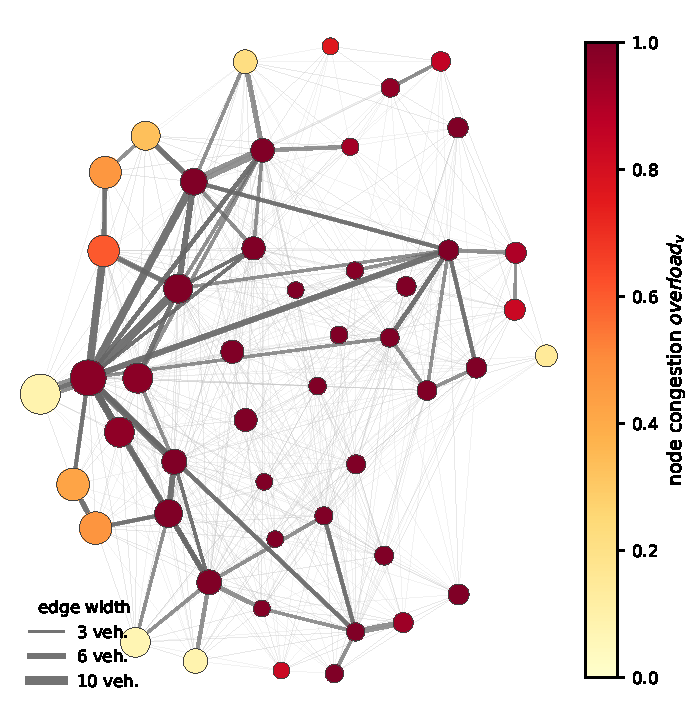
\includegraphics[height=0.46\textheight]{figs/germany_solution.pdf}

{\scriptsize Germany, $|V|=49$: a GVNS solution. Node area $=W_v$, colour $=$
congestion (dark $=$ at capacity), thick edges carry $\ge3$ vehicles.\par
\smallskip
\alert{A MIP solver given two hours returns a solution 54\% more expensive
than this one.}\par}
\end{columns}
\note{Say ``trucks'' and ``reload ceiling'', not ``MCND'' yet; say out loud
that we minimise vehicle movement cost plus reload cost. Point at the map:
thick edges are consolidated backbones, dark nodes are saturated storages. The
54\% is the ratio $1.544$ of Table~2, Germany, MIP-inc.\ column; the exact
budget at this size is 2\,h against a 98\,min limit for GVNS, of which it used
56\,min on average.}
\end{frame}

\begin{frame}{Feature 1: a road is billed per truck, not per unit}
\begin{columns}[T]
\column{0.5\textwidth}
\centering
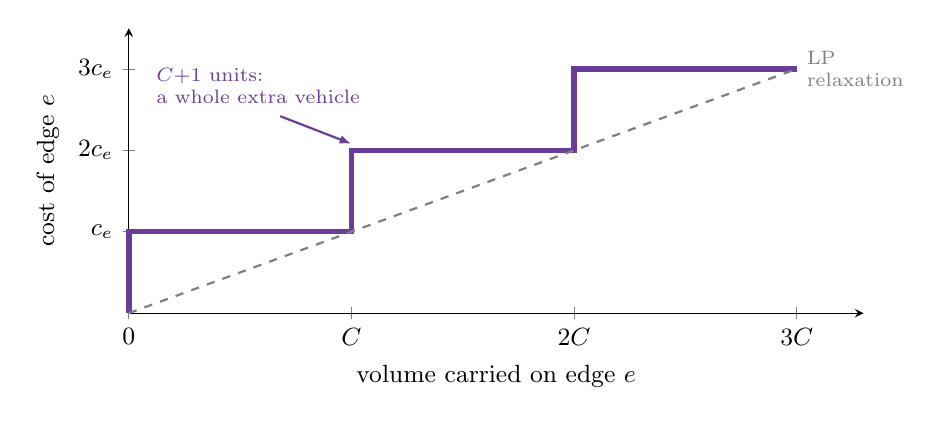
\begin{tikzpicture}
\begin{axis}[width=0.9\linewidth,height=5.2cm,xlabel={volume carried on edge $e$},ylabel={cost of edge $e$},
  xtick={0,50,100,150},xticklabels={0,$C$,$2C$,$3C$},ytick={1,2,3},yticklabels={$c_e$,$2c_e$,$3c_e$},
  ymin=0,ymax=3.5,xmin=0,xmax=165,axis lines=left,clip=false,label style={font=\small},tick label style={font=\small}]
\addplot[const plot mark right,line width=2pt,cStep] coordinates {(0,0)(0.01,1)(50,1)(50.01,2)(100,2)(100.01,3)(150,3)};
\addplot[dashed,gray,thick] coordinates {(0,0)(150,3)} node[pos=1,right,font=\scriptsize,text=gray,align=left] {LP\\relaxation};
\node[font=\scriptsize,text=cStep,align=left,anchor=south west] at (axis cs:4,2.45) {$C{+}1$ units:\\a whole extra vehicle};
\draw[-{Latex[length=1.5mm]},cStep,thick] (axis cs:34,2.42) -- (axis cs:50,2.08);
\end{axis}
\end{tikzpicture}

{\scriptsize schematic, $C=50$}
\column{0.5\textwidth}
\begin{block}{The billed quantity is the vehicle count}
\[
\text{cost of } e = \textcolor{cStep}{c_e\,y_e},\qquad y_e\in\Int_+
\]
with enough vehicles for the flow: $\sum_{k} x^k_e \le C\,y_e$
\end{block}
\begin{itemize}
\item a non-convex \emph{staircase} in the volume, shared by all requests on the edge
\item dropping integrality gives the line $c_e x/C$: the LP relaxation, polynomial but \emph{loose}
\end{itemize}
\end{columns}
\note{Practitioners recognise the staircase instantly; OR people recognise a
step-cost network design problem (Gabrel, Knippel, Minoux 1999; Croxton,
Gendron, Magnanti 2003). How loose: the LP solution with vehicles rounded up,
our starting solution, costs $1.19\times$ the GVNS solution at $|V|=10$,
$2.8\times$ at $|V|=50$ and $2.2$--$3.1\times$ at $|V|\ge90$ (Table~2).}
\end{frame}

\begin{frame}{Feature 2: every storage has a reload ceiling}
\begin{columns}[T]
\column{0.46\textwidth}
\centering
\begin{tikzpicture}[scale=0.72]
  \node[storage,minimum size=13mm,fill=cCap!60,font=\normalsize] (h) at (0,0) {$v$};
  \foreach \a/\c in {150/cN1,180/cN2,210/cOK} {\draw[flow,draw=\c] (\a:2.3) -- (h);}
  \foreach \a/\c in {30/cN1,0/cN2,-30/cOK} {\draw[flow,draw=\c] (h) -- (\a:2.3);}
  \draw[flow,draw=gray,dashed] (-2.4,-1.7) -- (-1.0,-1.0);
  \node[lbl,text=gray,align=left,anchor=north] at (-1.3,-1.85) {no room left:\\this request must detour};
  \draw[thick,mDarkTeal] (2.9,-0.9) rectangle (3.3,0.9);
  \fill[cCap!70] (2.9,-0.9) rectangle (3.3,0.9);
  \node[lbl,right] at (3.4,0.9) {$W_v$};
  \node[lbl,right,align=left] at (3.4,0.1) {transit flow\\$=W_v$};
  \node[lbl,right,text=cCap] at (3.4,-0.75) {$\ovl_v=1.0$};
\end{tikzpicture}

\medskip
{\small congestion of a storage in a solution:\\
$\ovl_v = \text{transit flow through } v\,/\,W_v$\\
$1.0$ = at capacity}
\column{0.54\textwidth}
\begin{block}{Transit volume through $v$ is bounded}
\[
\textcolor{cCap}{\sum_{k\in K:\,v\neq s_k,t_k}\ \sum_{e\in\delta^-(v)} x^k_e \;\le\; W_v}
\qquad\forall v\in V
\]
\end{block}
\begin{itemize}
\item once a storage is at capacity, further transit must detour: a longer route or a reload at a less loaded storage
\item origin and destination handling is not transshipment: a direct $s_k\!\to\!t_k$ route touches no node capacity
\end{itemize}
\end{columns}
\note{Node throughput bounds are familiar from hub location (Alumur \& Kara
2008), not from the MCND literature. $\ovl_v$ returns twice: it colours the
Germany map and it drives neighbourhood $N_3$.}
\end{frame}

\begin{frame}{Why not simply run a published network-design code?}   % [optional]
\centering
\footnotesize
\renewcommand{\arraystretch}{1.15}
\begin{tabular}{@{}l>{\raggedright\arraybackslash}p{4.6cm}>{\raggedright\arraybackslash}p{5.4cm}@{}}
\toprule
 & \textbf{fixed-charge capacitated MCND} & \textbf{this problem}\\
\midrule
arc cost & fixed charge per opened arc $+$ linear flow cost & \textcolor{cStep}{$c_e$ per vehicle: a staircase in the volume}\\
capacities & per arc & per arc (through vehicles) \textbf{and} \textcolor{cCap}{per node: transit volume $\le W_v$}\\
extra cost term & --- & reload $f_v$ per unit at every transit node\\
comparable published code & several (tabu, local branching, matheuristics) & none that we know of\\
\bottomrule
\end{tabular}

\medskip
\begin{alertblock}{Consequence for the experimental design}
no published network-design code that we know of charges per vehicle and bounds node throughput, and our open corpus has no published
objective values: we compare GVNS against \textbf{valid bounds} and \textbf{MIP solvers on the same model}
\end{alertblock}
\note{Skip in a 20-minute slot and say the consequence on the yardstick
slide. Literature, if asked (also on the backup slide ``Where it sits''):
capacitated MCND -- Gendron, Crainic, Frangioni 1999; Crainic 2000; column
generation / branch-and-price -- Barnhart et al.\ 1998; cycle-based tabu --
Ghamlouche, Crainic, Gendreau 2003; local branching -- Rodr\'iguez-Mart\'in \&
Salazar 2010; MILP-in-the-loop matheuristics -- Hewitt, Nemhauser, Savelsbergh
2010; survey -- Crainic \& Gendreau 2021. Step costs -- Gabrel, Knippel,
Minoux 1999; Croxton, Gendron, Magnanti 2003. Node capacity -- hub location,
Alumur \& Kara 2008. VNS -- Mladenovi\'c \& Hansen 1997; Hansen et al.\ 2017;
Hansen \& Mladenovi\'c 2019; multi-start VNS for single-path MCF -- Masri et
al.\ 2015; GVNS on CVRP -- Amous et al.\ 2017. Our own real-life logistic
heuristics: truck-and-trailer routing with time windows and split deliveries
(Batsyn \& Ponomarenko 2014, 2015).}
\end{frame}

% ---------------------------------------------------------------------------
\section{Model}

\begin{frame}{The model: an arc-based MILP}
\small
$x^k_e\in\Real_+$: flow of request $k$ on edge $e$;\quad
$y_e\in\Int_+$: vehicles on $e$;\quad $|K|\cdot|E|+|E|$ variables.
\vspace{-6pt}
\begin{align*}
\min\;& \textcolor{cStep}{\sum_{e\in E} c_e\,y_e}
 \;+\;\sum_{k\in K}\ \sum_{\substack{v\in V\\ v\neq s_k,t_k}}\ \sum_{e\in\delta^-(v)} f_v\,x^k_e
 &&\text{vehicles $+$ reloads}\\[-2pt]
\text{s.t.}\;&
\sum_{e\in\delta^+(v)} x^k_e-\sum_{e\in\delta^-(v)} x^k_e=
 \begin{cases} d_k & v=s_k\\ -d_k & v=t_k\\ 0 & \text{otherwise}\end{cases}
 && \forall k,\ \forall v \quad\text{(demand)}\\[-2pt]
&\textcolor{cStep}{\sum_{k\in K} x^k_e\le C\,y_e} && \forall e\in E \quad\text{(vehicle capacity)}\\
&\textcolor{cCap}{\sum_{k\in K:\,v\neq s_k,t_k}\ \sum_{e\in\delta^-(v)} x^k_e \le W_v} && \forall v\in V \quad\text{(transshipment capacity)}\\
& x\ge 0,\quad y\in\Int_+^{|E|}
\end{align*}
\vspace{-4pt}
linear objective and constraints, integer $y$, continuous $x$: a MILP, NP-hard.
This arc model is exactly what the exact solvers (HiGHS, SCIP) receive later.
\note{Read the equations once; every term was just seen in pictures. The
path-based twin has $\sum_k|\Pi_k|+|E|$ variables. Spoken bridge to the
method if the next frame is skipped: relaxing $y$ gives a per-unit path price,
travel$/C$ plus one reload per transit node, so the relaxation wants cheap
transit-free paths; that is why the start solution is every request on its
direct edge, and why $N_1$ searches with a reload-aware metric.}
\end{frame}

\begin{frame}{Path form, and what the LP relaxation tells us}   % [optional]
\begin{columns}[T]
\column{0.6\textwidth}
\textbf{Path form.} Flow $x^k_p$ on paths $p\in\Pi_k$ (all $s_k\!\to\!t_k$ paths),
$\sum_{p\in\Pi_k}x^k_p=d_k$, same $y_e$; only the paths that carry flow matter.

\medskip
\textbf{Relax integrality.} The capacity constraint becomes tight, so
$y_e=\frac1C\sum_k\sum_{p\ni e}x^k_p$ and $y$ disappears:
\[
\min\ \sum_{k\in K}\sum_{p\in\Pi_k} x^k_p\;
\underbrace{\Bigg(\frac1C\sum_{e\in p} c_e+\sum_{\substack{v\in p\\ v\neq s_k,t_k}} f_v\Bigg)}_{\text{per-unit price of path } p}
\]
\column{0.4\textwidth}
\centering
\begin{tikzpicture}
  \node[storage] (s) at (0,0) {$s$};
  \node[storage,fill=cCap!30] (v) at (2,0.9) {$v$};
  \node[storage] (t) at (4,0) {$t$};
  \draw[flow] (s) -- node[lbl,above left] {$c_{sv}/C$} (v);
  \draw[flow] (v) -- node[lbl,above right] {$c_{vt}/C$} (t);
  \node[lbl,text=cCap,above=1mm of v] {$+\,f_v$};
  \draw[road,dashed] (s) -- node[lbl,below] {$c_{st}/C$, no reload} (t);
\end{tikzpicture}

\medskip
\begin{block}{Reading}
a unit of flow pays \emph{travel}$/C$ plus one reload per transit node: the relaxation prefers cheap, transit-free paths
\end{block}
\end{columns}
\medskip
\begin{itemize}
\item on the completed graph the relaxed optimum puts every request on its direct edge: our \textbf{starting solution}; the search metric of $N_1$ is an edge-wise version of this price
\end{itemize}
\note{Bridge from model to method; skip in a 20-minute slot (the model frame's
note has the spoken version). $N_1$'s metric $c'_{vu}=f_v+f_u+c_{vu}/C$ is
edge-wise, so a transit reload is charged on both incident edges; it is a
ranking metric for path generation, not the objective---the MILP prices every
path exactly.}
\end{frame}

% ---------------------------------------------------------------------------
\section{The GVNS}

\begin{frame}{GVNS at a glance}
\centering
\begin{tikzpicture}[node distance=5mm and 6mm, box/.append style={text width=2.75cm,font=\scriptsize}]
  \node[box] (init) {\textbf{initial solution}\\rounded LP:\\every request on its direct edge};
  \node[box,right=of init,fill=cN2!15] (shake) {\textbf{Shake} in $N_k$\\diversified\\random paths\\MILP budget $\tau_{\mathrm{shk}}$};
  \node[box,right=11mm of shake,fill=cN1!15] (vnd) {\textbf{VND} $N_1\!\to\!N_2\!\to\!N_3$\\restart at $N_1$ on improvement\\MILP budget $\tau_{\mathrm{vnd}}$};
  \node[box,right=of vnd,text width=1.6cm] (test) {$z<z_0$?};
  \draw[road] (init) -- (shake);
  \draw[road] (shake) -- node[lbl,above=2pt,font=\scriptsize] {$z_0\gets z$} (vnd);
  \draw[road] (vnd) -- (test);
  \draw[road,draw=cOK] (test.south) -- ++(0,-0.55) -| node[pos=0.25,below,font=\scriptsize,text=cOK] {yes: $k\gets1$} (shake.south);
  \draw[road,draw=cN3] (test.south) -- ++(0,-1.15) -| node[pos=0.25,below,font=\scriptsize,text=cN3] {no: $k\gets k+1$} ($(shake.south)+(-0.5,0)$);
\end{tikzpicture}

\medskip
\begin{itemize}
\item \textbf{search space: commodity paths.} A solution is a path pool $P$ with flows $x$; vehicle counts follow, $y_e=\big\lceil\frac1C\sum_k x^k_e\big\rceil$
\item \textbf{shake and VND are the same primitive} (next slide): the shake adds more, random paths with a larger MILP budget
\item \textbf{stop} when $k>3$ or after $t_{\max}=2|V|$ minutes; a move is accepted \emph{only if it improves}, so the shake never degrades the incumbent, and $k$ advances when the VND fails to beat the post-shake value $z_0$
\end{itemize}
\note{Preprocessing: complete the graph, build the reload-aware graph $G'$,
precompute 20 shortest paths per request. Shake vs VND path counts: 5 random
pool paths vs 1--3 for $N_1$; stop at 3 fully loaded paths / $5C$ free room vs 2 / $1C$ for $N_2$;
3 detours vs 1 for $N_3$. Budgets: $\tau_{\mathrm{shk}}=10+|V|$ / $100+2|V|$\,s,
$\tau_{\mathrm{vnd}}=25$ / $70$\,s ($N_1$ / rest; 15 / 50\,s at $|V|=100$), so
for $N_1$ the shake budget is smaller than the VND budget while $|V|\le14$.
A VNS-school listener will ask whether this is a shake: it is Algorithm~1
called with diversified generation and $\tau_{\mathrm{shk}}$; diversification
comes from the random paths pushed into the pool and the MILP re-optimisation,
and a non-improving shake is discarded. All parameters are on the backup slide
``Settings''.}
\end{frame}

\begin{frame}{Preprocessing and the starting solution}   % [optional]
\begin{columns}[T]
\column{0.5\textwidth}
\centering
\begin{tikzpicture}[scale=0.68]
  \node[storage] (a) at (0,0) {$a$};
  \node[storage] (b) at (1.6,1.2) {$b$};
  \node[storage] (c) at (3.2,0.2) {$c$};
  \node[storage] (d) at (1.8,-1.2) {$d$};
  \draw[road] (a) -- (b); \draw[road] (b) -- (c); \draw[road] (a) -- (d); \draw[road] (d) -- (c);
  \node[lbl,text=black] at (1.6,-2.0) {(a) raw road graph};
  \begin{scope}[xshift=6.0cm]
  \node[storage] (a2) at (0,0) {$a$};
  \node[storage] (b2) at (1.6,1.2) {$b$};
  \node[storage] (c2) at (3.2,0.2) {$c$};
  \node[storage] (d2) at (1.8,-1.2) {$d$};
  \draw[road] (a2) -- (b2); \draw[road] (b2) -- (c2); \draw[road] (a2) -- (d2); \draw[road] (d2) -- (c2);
  \draw[road,dashed,draw=cN1] (a2) -- node[lbl,text=cN1,above,pos=0.78] {$c_{ac}$} (c2);
  \draw[road,dashed,draw=cN1] (b2) -- (d2);
  \node[lbl,text=black] at (1.6,-2.0) {(b) completed graph};
  \end{scope}
\end{tikzpicture}
\column{0.5\textwidth}
\begin{itemize}
\item road graphs are sparse ($a\!\to\!c$ needs a stop); on the raw graph a missing origin--destination path can even make an instance infeasible
\item \textbf{completion}: join every ordered pair by an edge costing the shortest path in $G$ ($c_{ac}$): the cheapest \emph{stop-free} route, touching no $W_v$
\item the exact solvers get the same completed graph ($|E|=|V|(|V|-1)$)
\end{itemize}
\end{columns}
\smallskip
\begin{block}{Start: the rounded LP}
every request on its direct edge (the relaxed optimum), vehicles rounded up: always feasible, and poor ($1.19\times$ GVNS at $|V|=10$, $2.80\times$ at 50, $3.14\times$ on European Russia)
\end{block}
\note{Skip in a 20-minute slot: say ``we complete the graph so every request
has a direct stop-free edge, and start from the rounded LP''. On the raw graph
the node capacities also shrink the feasible region (paper, Sec.~3.2). Many of the
trucks on those direct edges leave partly empty---that is what $N_2$ will fix.
The initial MILP that sets up the flows has a 300\,s limit.}
\end{frame}

\begin{frame}{The move primitive: propose paths, let the MILP redistribute}
\centering
\begin{tikzpicture}[node distance=5mm]
  \node[box,fill=cN1!10] (gen) {\textbf{GenPaths}$(N,k)$\\new candidate paths $Q$\\for every request $k$};
  \node[box,right=of gen] (milp) {\textbf{MILP} on pool $P\cup Q$\\redistribute flow: warm start $x$,\\time limit $\tau$, gap 1\%};
  \node[box,right=of milp,fill=cOK!10] (keep) {improved ($z'<z$)?\\keep new paths with $x'_p>0$,\\prune every zero-flow path};
  \node[box,below=3mm of keep,fill=cCap!10,text width=3.6cm] (drop) {not improved: discard $Q$};
  \draw[road] (gen) -- (milp);
  \draw[road] (milp) -- (keep);
  \draw[road] (milp.east) -- ++(0.35,0) |- (drop.west);
\end{tikzpicture}

\medskip
\begin{columns}[T]
\column{0.5\textwidth}
\begin{block}{Why paths and not edge flows}
per-edge flows are strongly coupled across requests, so a feasible change needs the whole network at once; a path describes one request only, and \emph{adding} a path to a feasible solution never makes it worse
\end{block}
\column{0.5\textwidth}
\begin{itemize}
\item the three neighbourhoods differ \emph{only} in \textbf{GenPaths}; everything else is shared
\item pruning zero-flow paths keeps the in-loop MILP small enough for budgets of 25--70\,s (VND) and $10{+}|V|$ to $100{+}2|V|$\,s (shake)
\item the neighbourhood proposes, the MILP disposes
\end{itemize}
\end{columns}
\note{This is the matheuristic core; OR people will map it to MILP-in-the-loop
schemes (Hewitt et al.). The MILP is HiGHS with a 1\% gap target.}
\end{frame}

\begin{frame}{\textcolor{cN1}{$N_1$}: reload-aware shortest paths}
\begin{columns}[T]
\column{0.45\textwidth}
\centering
\begin{tikzpicture}[scale=1.15]
  \node[storage] (s) at (0,0) {$s$};
  \node[storage,fill=cCap!30] (h) at (2.2,1.1) {$h$};
  \node[storage] (t) at (4.4,0) {$t$};
  \draw[road,draw=cN1,line width=1.5pt] (s) -- node[lbl,above left,text=cN1] {$c'_{sh}$} (h);
  \draw[road,draw=cN1,line width=1.5pt] (h) -- node[lbl,above right,text=cN1] {$c'_{ht}$} (t);
  \draw[road,draw=cN1,line width=1.5pt] (s) -- node[lbl,below,text=cN1] {$c'_{st}$} (t);
  \foreach \i in {1,...,6} {\draw[cN1!30,line width=0.6pt] (0.2,-0.9-0.13*\i) -- (3.0,-0.9-0.13*\i);}
  \foreach \i in {1,2,3} {\draw[cN1,line width=1pt] (0.2,-0.9-0.13*\i) -- (3.0,-0.9-0.13*\i);}
  \node[lbl,right,text=cN1,align=left] at (3.1,-1.35) {pool of 20 paths\\per request};
\end{tikzpicture}
\column{0.55\textwidth}
\begin{block}{Auxiliary complete graph $G'$: per-unit weights}
\[
c'_{vu}=f_v+f_u+\frac{c_{vu}}{C}\qquad\forall (v,u)\in E
\]
travel per unit plus the reloads at the endpoints; plain shortest paths would ignore the reloads
\end{block}
\begin{itemize}
\item 20 shortest paths per request under $c'$, precomputed once; new paths come from this pool
\item \textbf{VND}: $\{1,2,3\}$ new paths per request $\times$ \{random, low-cost first\}; \textbf{Shake}: 5 random pool paths
\item ablation: without $N_1$, $+0.8\%$ (median, synthetic and real alike)
\end{itemize}
\end{columns}
\note{Keep short: $N_2$ is where the money is. If a sharp listener notes that
$c'$ charges a transit reload on both incident edges and also prices origin
and destination reloads: $c'$ is a ranking metric for path generation, not the
objective; the MILP prices every path exactly, so the double count only changes
which 20 paths enter the pool.}
\end{frame}

\begin{frame}{\textcolor{cN2}{$N_2$}: fill the half-empty trucks}
\begin{columns}[T]
\column{0.46\textwidth}
\centering
\begin{tikzpicture}[x=1cm,y=1cm,scale=0.8]
  \node[font=\footnotesize] at (2.7,1.35) {edge $(u,v)$: 110 units, $y_{uv}=\lceil 110/50\rceil=3$};
  \foreach \i/\l in {0/50, 1/50, 2/10} {
    \draw[thick,mDarkTeal] (\i*1.9,0) rectangle ++(1.6,0.7);
    \fill[cN1!60] (\i*1.9,0) rectangle ++(1.6*\l/50,0.7);
    \node[font=\scriptsize] at (\i*1.9+0.8,-0.3) {\l\,/\,50};
  }
  \draw[{Latex}-{Latex},cN2,line width=1.5pt] (3.8+0.33,0.35) -- (3.8+1.58,0.35);
  \node[font=\scriptsize,text=cN2,align=center] at (4.75,0.95) {40 units free};
  \node[font=\footnotesize,align=center] at (2.7,-1.15) {$\load_{uv}=110 \bmod 50 = 10$:\\up to 40 more units here cost \textbf{no extra vehicle}\\and may free one elsewhere};
\end{tikzpicture}

\medskip
\begin{itemize}
\item shortest paths on $G''$ run through partially loaded vehicles
\item dynamic number of new paths per request: stop after 2 fully loaded paths or accumulated free room $\ge1C$ (VND); 3 fully loaded paths or $\ge5C$ (Shake)
\end{itemize}
\column{0.54\textwidth}
\begin{block}{Graph $G''$ favours free room ($\alpha=0.5$)}
\small
\begin{gather*}
c''_{vu}=f_v+f_u+\frac{\load_{vu}}{C}\Big(\frac{c_{vu}}{C}\Big)^{\!\alpha}\\[-2pt]
\load_e=\Big(\textstyle\sum_k\sum_{p\ni e}x^k_p\Big)\bmod C
\end{gather*}
fully loaded edges ($\load_e=0$) keep their $G'$ weight; smaller residual load $\Rightarrow$ lower weight
\end{block}
\begin{alertblock}{Ablation: the dominant operator}
without $N_2$: $+3.9\%$ synthetic, $+1.6\%$ real (medians), up to $+23.8\%$ on a single instance
\end{alertblock}
\end{columns}
\note{Slow down here. Vehicle consolidation is the main lever on the
objective. On the synthetic ablation subset the mean loss is $+7.1\%$ and the
worst case $+23.8\%$ (50\_nodes\_2); on the real subset the mean is $+2.6\%$
and Germany loses $7.6\%$ (components\_A.csv); none of these is corpus-wide.}
\end{frame}

\begin{frame}{\textcolor{cN3}{$N_3$}: detour around the saturated storage}
\begin{columns}[T]
\column{0.48\textwidth}
\centering
\begin{tikzpicture}
  \node[storage] (a) at (0,0) {$s$};
  \node[storage,minimum size=10mm,fill=cCap!70] (b) at (2.4,0) {$v^\ast$};
  \node[storage] (c) at (4.8,0) {$t$};
  \node[storage,fill=cN1!20] (d) at (2.4,-1.6) {$w$};
  \draw[road] (a) -- (b); \draw[road] (b) -- (c);
  \draw[cCap,line width=1.5pt] (b.north west) -- (b.south east); \draw[cCap,line width=1.5pt] (b.north east) -- (b.south west);
  \draw[flow] (a) to[bend right=25] (d); \draw[flow] (d) to[bend right=25] (c);
  \node[lbl,text=cCap,above=1.5mm of b] {$\ovl_{v^\ast}\approx1$: removed from $G'$};
  \node[lbl,below=1mm of d] {new shortest path through a less loaded $w$};
\end{tikzpicture}

\medskip
{\small in the current solution:\\[2pt]
$\ovl_v=\dfrac1{W_v}\displaystyle\sum_{k:\,v\neq s_k,t_k}\ \sum_{p\in\Pi_k:\,v\in p}x^k_p$}
\column{0.52\textwidth}
\begin{itemize}
\item delete the \textbf{single most congested} storage from $G'$ (unless it is the request's own origin or destination), recompute the shortest path: a detour to less loaded storages
\item 1 new path per request in VND, 3 in Shake
\item ablation: $+0.1\%$ / $+0.2\%$ median, \textbf{inactive when capacities are slack}; $+4.0\%$ on Germany, where almost every storage runs at capacity
\end{itemize}
\end{columns}
\note{Say ``situational'' out loud: the operator is worth carrying only for
tight instances---when capacities are slack there is nothing to route around.
Point back at the Germany map. If asked why a single node: removing a prefix
of $|V|/5$--$|V|/4$ congested storages was tried on all 50 instances $\times$
10 seeds; it is indistinguishable on 44 of 50 (within across-seed noise) yet
forfeits $N_3$'s benefit on the capacity-tight networks, so the surgical
version is kept---state the measured outcome, not a mechanism.}
\end{frame}

% ---------------------------------------------------------------------------
\section{Experiments}

\begin{frame}{The benchmark: realistic regional networks, openly available}
\begin{columns}[T]
\column{0.56\textwidth}
\begin{itemize}
\item our open corpus (arXiv:2606.20653; Zenodo, CC-BY-4.0), every instance reproducible from its published seed
\item road networks between regional sorting centres, calibrated on OpenStreetMap for \textbf{nine European countries, five U.S.\ states and European Russia}
\item real structure: Zipf city sizes, spatial-network topology, centrality-driven $W_v$, gravity demand; near-planar, large-diameter graphs
\item \textbf{35 synthetic}: $10\times|V|{=}10$, $7\times20$, $7\times30$, $5\times50$, $3\times100$, $3\times150$
\item \textbf{15 real-geometry}: Denmark ($|V|=11$) to European Russia ($|V|=90$)
\end{itemize}
\column{0.44\textwidth}
\centering
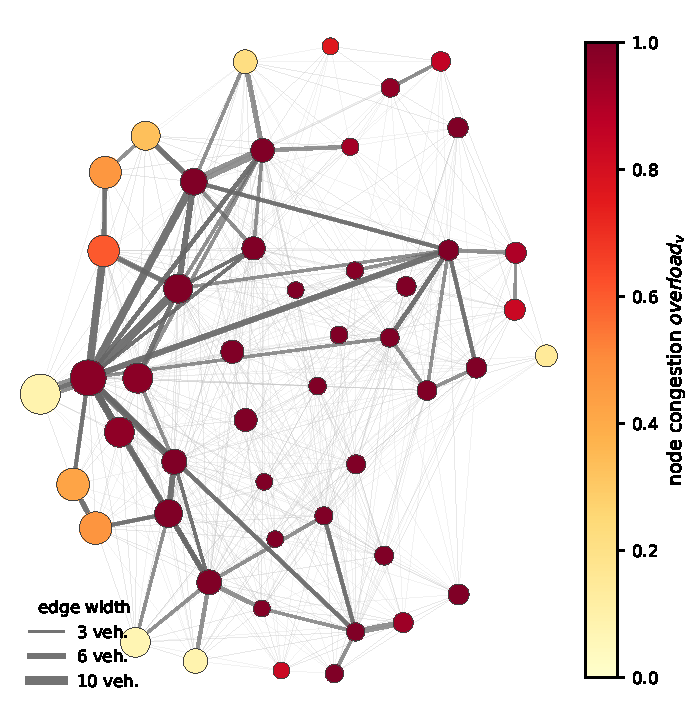
\includegraphics[height=0.52\textheight]{figs/germany_solution.pdf}

{\scriptsize Germany ($|V|=49$), the solution from the first slide:
almost every storage runs at capacity.\par}
\end{columns}
\note{The generator is a separate paper; here only what the study needs.
Mean degree is 3.575 in the paper. Point at the map: thick edges are
consolidation ($N_2$) made visible, dark nodes are what $N_3$ works on. The
instance's numbers come where they are defined: $\gapLB=11.0\%$, exact
incumbent $1.544\times$, rounded-LP start $2.692\times$, $\sigma$ over 10 seeds
$2.0\%$; without $N_2$ $+7.6\%$, without $N_3$ $+4.0\%$.}
\end{frame}

\begin{frame}{Setup and yardsticks}
\centering
\begin{tikzpicture}[x=1cm]
  \draw[-{Latex[length=2.5mm]},thick,mDarkTeal] (0,0) -- (13.2,0) node[right,font=\scriptsize] {objective};
  \foreach \x/\lab/\val/\col in {0.9/{LP relaxation}/{0.971}/gray, 3.6/{MIP dual bound $\underline{z}$}/{}/cN1, 6.2/{optimum $z^\ast$}/{(unknown)}/gray, 8.8/{GVNS}/{1.0}/mLightBrown, 11.8/{rounded LP (start)}/{1.192}/gray}{
    \draw[thick,\col] (\x,-0.15) -- (\x,0.15);
    \node[font=\scriptsize,text=\col,align=center,above=1mm] at (\x,0.15) {\lab\\ \val};
  }
  \node[font=\scriptsize,text=cOK,align=center,below=1mm] at (8.8,-0.15) {MIP incumbent 1.000};
  \draw[{Bar}-{Bar},thick,cN1] (3.6,-0.75) -- (8.8,-0.75) node[midway,below,font=\scriptsize,text=cN1] {$\gapLB=0.96\%$};
  \node[font=\scriptsize,text=gray] at (11.8,-0.8) {ratios: means at $|V|=10$; not to scale};
\end{tikzpicture}

\smallskip
\begin{columns}[T]
\column{0.48\textwidth}
\begin{block}{Two metrics}
\small
$\gapLB=\big(\mathit{Result}_{\mathrm{GVNS}}-\underline{z}\big)/\underline{z}$,\quad $\underline{z}=$ best MIP dual bound:
an \textbf{upper bound on the true optimality gap} of GVNS\\[3pt]
$\mathit{Ratio}_{\mathrm{method}}=\mathit{Result}_{\mathrm{method}}/\mathit{Result}_{\mathrm{GVNS}}$:
below 1 better than GVNS, above 1 worse
\end{block}
\column{0.52\textwidth}
\begin{itemize}\small
\item GVNS: 10 seeds per instance, limit $2|V|$\,min; exact: gap target 0, 30\,min--4\,h, i.e.\ comparable budgets ($|V|=50$: 100\,min vs 2\,h); HiGHS is the exact baseline \emph{and} the in-loop solver
\item nothing is proven optimal, but $\underline{z}$ is a valid lower bound, typically within a few percent of the incumbent: $\gapLB$ is a guarantee, not a self-comparison
\end{itemize}
\end{columns}
\note{Hardware: HSE cluster cHARISMa, nodes with 2$\times$AMD EPYC (44 cores,
$\ge$720\,GB RAM), each job pinned to 8 cores; HiGHS 1.14.0, SCIP 10.0.2 as
cross-check. Exact side in one breath: none of the 50 instances was solved to
proven optimality; up to $|V|=42$ the two solvers' dual bounds agree within
$0.6\%$; SCIP returns nothing usable from $|V|=45$; the arc model is out of
memory at $|V|\ge100$ (backup ``The exact side''). If you accept one number
from this talk, make it $\gapLB$: it bounds the distance to the optimum instead
of comparing GVNS with itself. The ladder ticks are the $|V|=10$ means of
Table~2; the dual bound sits between the LP and GVNS, and GVNS is $0.96\%$
above it.}
\end{frame}

\begin{frame}{Results I: synthetic instances}
\begin{columns}[T]
\column{0.56\textwidth}
\centering
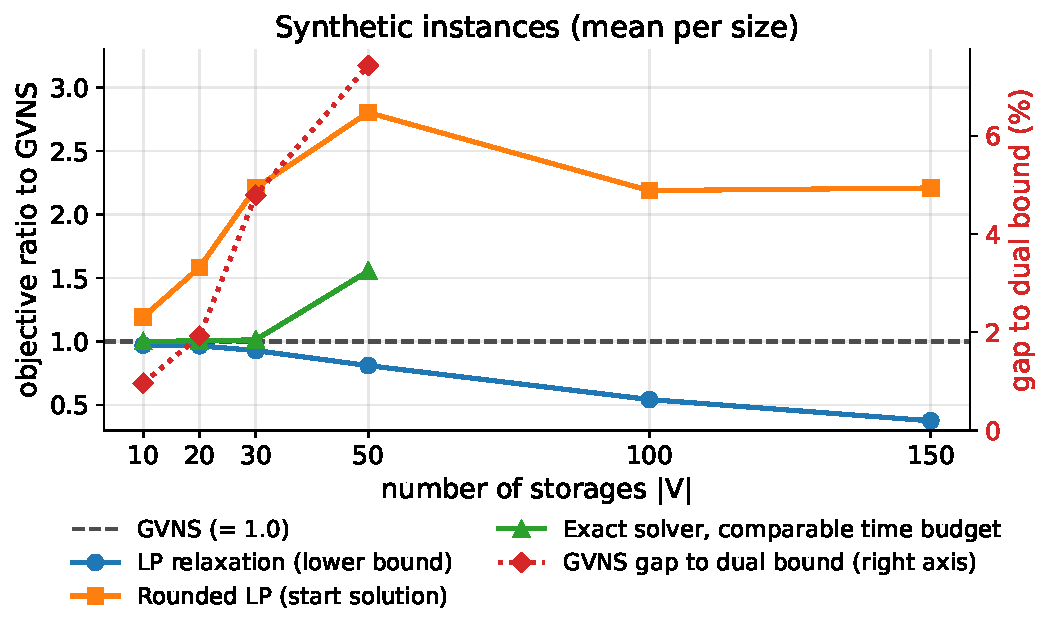
\includegraphics[width=0.94\linewidth]{figs/ratios_synthetic.pdf}
\column{0.44\textwidth}
\centering
\small
\setlength{\tabcolsep}{4pt}
\begin{tabular}{@{}rrccc@{}}
\toprule
$|V|$ & $n$ & $\gapLB$ & exact inc. & $\sigma$\\
\midrule
10  & 10 & 0.96\% & 1.000 & 0.06\%\\
20  & 7  & 1.92\% & 1.005 & 0.18\%\\
30  & 7  & 4.79\% & 1.013 & 0.68\%\\
50  & 5  & 7.44\% & \alert{1.555} & 0.66\%\\
100 & 3  & \dag & \dag & 0.31\%\\
150 & 3  & \dag & \dag & 0.38\%\\
\bottomrule
\end{tabular}

{\scriptsize\dag: arc model intractable; only the loose LP bound (0.542, 0.375)\par}

\smallskip
{\small near-optimal up to $|V|=20$; at $|V|=50$ the exact solver with a comparable budget is \alert{55\% more expensive} on average (16\% to 137\% per instance)\par}
\end{columns}
{\scriptsize GVNS mostly stops before its limit (3\,729 of 6\,000\,s at $|V|=50$); the exact solver always used its full budget, so the comparison is conservative.\par}
\note{Trace the green curve: flat at 1.0, up to 1.555 at 50, then it stops
existing. Spoken: $\gapLB$ is about 1--2\% up to $|V|\approx20$, 4.8\% at 30,
7.4\% at 50, where the LP bound alone would say about 24\%; at $|V|\ge100$
GVNS still ends $2.2\times$ below its own start. Mean run time vs limit:
633/1\,200\,s (10), 1\,952/2\,400 (20), 2\,611/3\,600 (30), 3\,729/6\,000 (50),
5\,983/12\,000 (100), 18\,236/18\,000 (150); the 150-node mean slightly exceeds
its limit because Algorithm~2 tests $t_{\max}$ only before each shake and after
each full VND sweep, so a shake started just under the limit (MILP budget up to
$100+2|V|=400$\,s at $|V|=150$) and the sweep after it run to completion.
Per-instance $|V|=50$ numbers are on the backup slide ``What the means hide''.}
\end{frame}

\begin{frame}{Results II: real road geometries mirror the synthetic story}
\begin{columns}[T]
\column{0.58\textwidth}
\centering
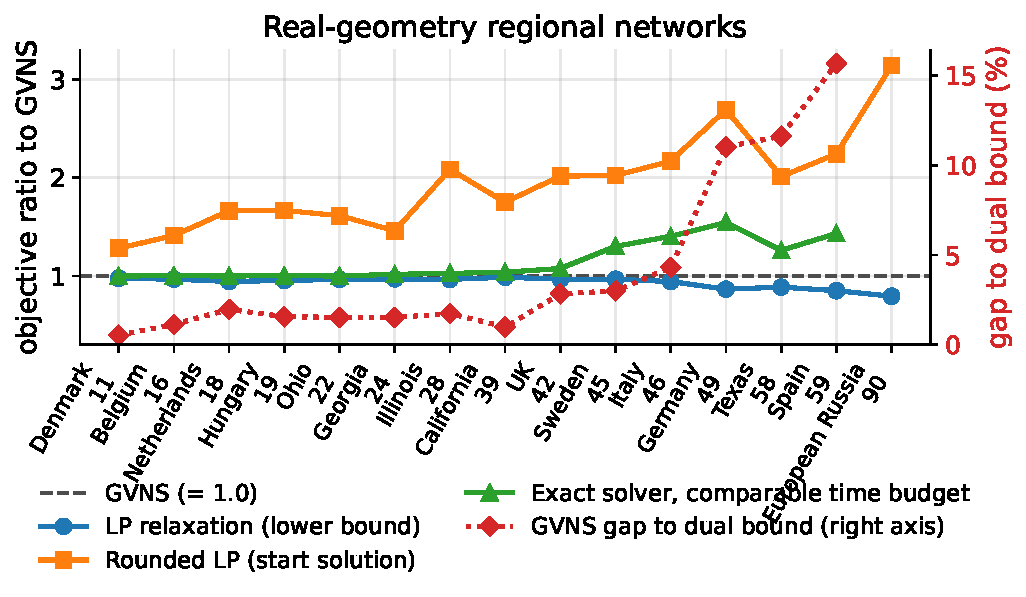
\includegraphics[width=\linewidth]{figs/ratios_real.pdf}
\column{0.42\textwidth}
\begin{itemize}
\item exact solver with a comparable budget: parity up to $|V|=22$, $1.02$--$1.08\times$ up to the UK (42), then \alert{$1.26$--$1.54\times$} from Sweden (45) to Spain (59)
\item $\gapLB$ from $0.5\%$ (Denmark, 11) to $15.7\%$ (Spain, 59)
\item European Russia ($|V|=90$): no exact reference; GVNS ends $3.1\times$ below its start
\end{itemize}
\medskip
{\small\itshape same shape as the synthetic curves: the synthetic corpus behaves like the real geometries, and GVNS is robust to them}
\end{columns}
\note{Do not read the table; point at the three medium networks and at the
90-node one. Spoken detail: $\gapLB$ about 1--3\% up to $|V|=45$, 4.3\% on
Italy (46), 11.0\% Germany (49), 11.6\% Texas (58), 15.7\% Spain (59); exact
incumbent 1.02--1.04$\times$ from Georgia (24) to California (39), 1.077 UK;
run time 615\,s (Denmark) to 3\,986\,s (Spain), 5\,595\,s on European Russia.
Full Table~2 rows are in the paper.}
\end{frame}

\begin{frame}{How many seeds do you need?}   % [optional]
\begin{columns}[T]
\column{0.58\textwidth}
\centering
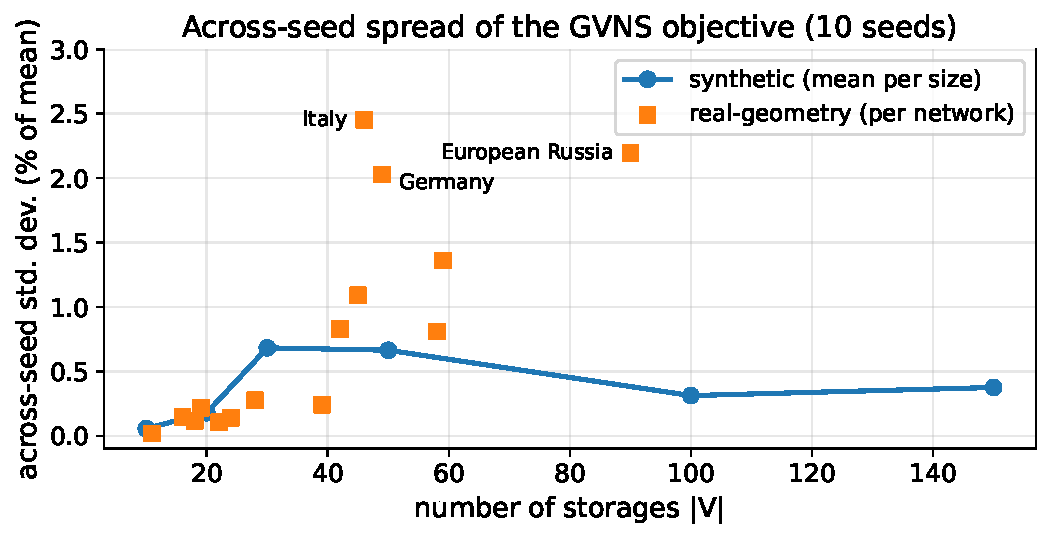
\includegraphics[width=\linewidth]{figs/seed_spread.pdf}
\column{0.42\textwidth}
\begin{itemize}
\item synthetic: across-seed $\sigma$ below $0.7\%$ of the mean at every size, below $0.2\%$ up to $|V|=20$
\item large real networks: $2.0\%$ (Germany), $2.5\%$ (Italy), $2.2\%$ (European Russia)
\item \alert{three seeds badly understate it}: on Italy the spread over three seeds is $0.4\%$ against $2.5\%$ over ten
\item one run is representative on small networks; on capacity-tight instances take the best of several
\end{itemize}
\end{columns}
\note{Backup for the ``is it stable?'' question. We moved from 3 to 10 seeds
for the headline numbers and 5 for the component study.}
\end{frame}

\begin{frame}{What each component buys}
\begin{columns}[T]
\column{0.54\textwidth}
\centering
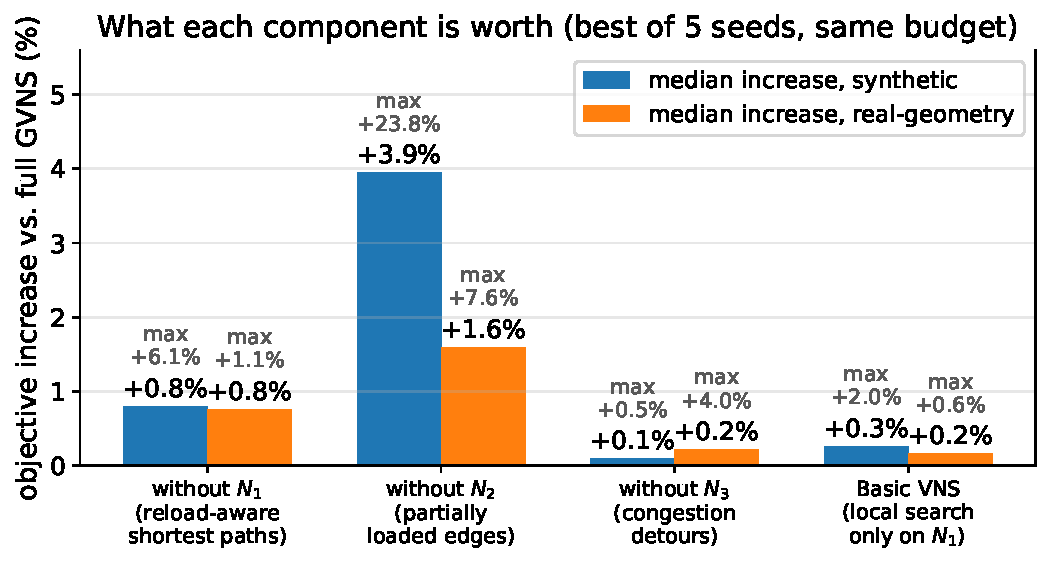
\includegraphics[width=\linewidth]{figs/ablation.pdf}

{\scriptsize best of 5 seeds, same budget, subset of synthetic ($|V|=20$--$100$) and real ($16$--$49$) instances; medians because the seed spread is heavy-tailed on capacity-tight networks\par}
\column{0.46\textwidth}
\footnotesize
\setlength{\tabcolsep}{3pt}
\begin{tabular}{@{}lcc@{}}
\toprule
GVNS better / tie / variant better & synth. & real\\
\midrule
without $N_1$ & 8 / 0 / 1 & 5 / 1 / 0\\
without $N_2$ & 8 / 1 / 0 & 5 / 1 / 0\\
without $N_3$ & 1 / 8 / 0 & 3 / 3 / 0\\
Basic VNS & 5 / 4 / 1 & 2 / 4 / 0\\
\bottomrule
\end{tabular}

{\scriptsize ``decided'' = difference beyond the seed spread of both runs; time relative to GVNS: 0.80, 0.52, 0.68, 0.63\par}

\medskip
\begin{itemize}\small
\item \textcolor{cN2}{$N_2$ dominates}; \textcolor{cN3}{$N_3$ is situational}: ties when capacities are slack, $+4.0\%$ on Germany
\item \textbf{Basic VNS} (local search on $N_1$ only, same shake): GVNS better on 7 of 16, Basic VNS on 1, 8 ties; the margin grows with size, $0.2$--$0.6\%$ at $|V|\le28$ vs $1.1$--$2.0\%$ at $|V|\ge50$, for $1/0.63$ of the time
\end{itemize}
\end{columns}
\note{One line: $N_2$ dominates, the VND matters at scale, $N_3$ is for tight
instances. Table~3's time ratios are the means of the synthetic and real
groups (CSV: $N_1$ 0.76/0.84, $N_2$ 0.54/0.50, $N_3$ 0.73/0.63, Basic VNS
0.68/0.58). The CSV's \texttt{argmax\_instance} names the instance where the
variant is \emph{worst}, not best. Single instances can flip sign: the two
``variant better'' entries in the table are decided (beyond the seed spread of
both runs): 50\_nodes\_2, where dropping $N_1$ improved the result by 2.1\%, and
30\_nodes\_2, where Basic VNS beat GVNS by 1.3\%; Basic VNS also improves
Germany by 4.0\%, but inside its 4.2\% seed spread there, so a tie.}
\end{frame}

% ---------------------------------------------------------------------------
\section{Closing}

\begin{frame}{Limitations, and what comes next}
\begin{columns}[T]
\column{0.5\textwidth}
\textbf{Stated before you ask}
\begin{itemize}\small
\item \textbf{static capacities and costs}: on real networks they vary with the time of day
\item \textbf{no proven optima}: $\gapLB$ is an upper bound on the true gap
\item \textbf{no tight reference beyond $|V|=59$}: only the loose LP bound
\item \textbf{path generation is heuristic}: a pool of 20 shortest paths plus three rules
\item \textbf{open-source solvers at default settings} as the exact baseline (tuning checked on 8 instances)
\item \textbf{component study} on a subset with five seeds; \textbf{no operational data} yet
\end{itemize}
\column{0.5\textwidth}
\textbf{Next}
\begin{itemize}\small
\item time-expanded graph with period-dependent $C_e(t)$, $W_v(t)$: the neighbourhoods only need a period-aware edge metric
\item column-generation pricing to feed the path pool
\item validation on operational data
\end{itemize}
\end{columns}
\note{Justifications, spoken: at $|V|=50$--$59$ the 7--16\% gap cannot be split
between heuristic error and bound weakness; beyond $|V|=59$ the LP bound is
0.795 on European Russia and 0.542 / 0.375 at 100 / 150; HiGHS and SCIP with
three presets each moved nothing (backup ``The exact side''). The ``next''
items answer the first, fourth and last limitations.}
\end{frame}

\begin{frame}{Takeaways}
\begin{enumerate}\setlength{\itemsep}{8pt}
\item \textcolor{cStep}{integer trucks} $+$ \textcolor{cCap}{reload ceilings}: compare against \textbf{valid dual bounds}, not fixed-charge codes
\item path-space GVNS: within $\approx1\%$ of the dual bound on small networks; the exact solver is \textbf{up to 55\% more expensive} at $|V|=50$
\item \textcolor{cN2}{$N_2$} is the lever, \textcolor{cN3}{$N_3$} only when capacity binds, the full VND pays at scale
\end{enumerate}
\bigskip
\begin{center}
{\large\itshape Let cheap path generators propose and a time-boxed MILP dispose:\\
$N_2$ always, $N_3$ when capacity binds, the full VND once the network is large.}
\end{center}
\note{End on the italic sentence; it calls back to ``the neighbourhood
proposes, the MILP disposes'' on the primitive slide.}
\end{frame}

\begin{frame}{Thank you}
\begin{columns}[T]
\column{0.58\textwidth}
\textbf{Code, exact-solver harness, scripts that regenerate every table and figure}\\
{\small\href{https://github.com/aponom84/Optimal-Logistic-Net}{\texttt{github.com/aponom84/Optimal-Logistic-Net}}}

\medskip
\textbf{Instance corpus} (CC-BY-4.0)\\
{\small\href{https://doi.org/10.5281/zenodo.20372456}{\texttt{doi.org/10.5281/zenodo.20372456}}}

\medskip
\textbf{Contact}\\
\texttt{aponomarenko@hse.ru} $\cdot$ \texttt{varvara\_kovaleva03@mail.ru}

\bigskip
{\footnotesize Supported by the Basic Research Program at HSE University
(HSE-BR-2025-080) and by the HPC facilities of HSE University (cHARISMa).\par}
\column{0.42\textwidth}
\centering
\begin{tabular}{c@{\hspace{6mm}}c}
\qrcode[height=2.4cm]{https://github.com/aponom84/Optimal-Logistic-Net} &
\qrcode[height=2.4cm]{https://doi.org/10.5281/zenodo.20372456}\\[3pt]
{\small code} & {\small data}
\end{tabular}
\end{columns}
\note{Question map: seeds -- ``How many seeds''; solver behaviour and tuning --
backup ``The exact side''; per-instance spread at $|V|=50$ -- backup ``What
the means hide''; any parameter -- backup ``Settings''; literature -- backup
``Where it sits''; the $N_3$ prefix variant -- the $N_3$ slide's note.}
\end{frame}

% ---------------------------------------------------------------------------
% Backup slides: no progress bar (its denominator is the appendix frame
% count, which appendixnumberbeamer only knows after the first pass).
\appendix
\metroset{progressbar=none}

\begin{frame}{Backup: settings (Table~1 of the paper)}
\centering
\small
\renewcommand{\arraystretch}{1.15}
\setlength{\tabcolsep}{4pt}
\begin{tabular}{llll}
\toprule
Setting & Value & Setting & Value\\
\midrule
neighbourhoods $k_{\max}$ & 3 & $N_2$ exponent $\alpha$ & 0.5\\
GVNS limit $t_{\max}$ & $2|V|$\,min & $N_2$ free-room stop & $1C$ / $5C$\\
random seeds & 10 / 5 (components) & $N_3$ storages removed & 1 (most congested)\\
vehicle capacity $C$ & 50 & $N_1$ path pool & 20\\
$N_1$ paths per request & 1--3 / 5 & $N_3$ paths per request & 1 / 3\\
initial MILP limit & 300\,s & exact gap target & 0\\
redistribution MILP gap & 1\% & exact budget & 30\,min--4\,h\\
$\tau_{\mathrm{shk}}$ ($N_1$ / rest) & $10{+}|V|$ / $100{+}2|V|$\,s & $\tau_{\mathrm{vnd}}$ ($N_1$ / rest) & 25 / 70\,s ($15$ / $50$\,s at $|V|=100$)\\
\bottomrule
\end{tabular}

\medskip
{\footnotesize Values given as VND / Shake where they differ. Each job pinned to 8 cores;
HSE cluster cHARISMa (2$\times$AMD EPYC, 44 cores, $\ge$720\,GB RAM per node); HiGHS 1.14.0, SCIP 10.0.2.}
\end{frame}

\begin{frame}{Backup: the exact side, and is the baseline understated?}
\centering
\scriptsize
\renewcommand{\arraystretch}{1.05}
\begin{tabular}{@{}l>{\raggedright\arraybackslash}p{4.2cm}>{\raggedright\arraybackslash}p{4.6cm}>{\raggedright\arraybackslash}p{3.2cm}@{}}
\toprule
 & \textbf{HiGHS 1.14} & \textbf{SCIP 10} & \textbf{arc MILP size}\\
\midrule
$|V|\le 42$ & dual bound $+$ incumbent & dual bound agrees with HiGHS within $0.6\%$ (mean $0.18\%$); weaker incumbent & $\approx6\,000$ variables at $|V|=10$\\
$|V|=45$--$59$ & dual bound $+$ incumbent & \textcolor{cCap}{no feasible solution, no non-trivial bound} & \\
$|V|\ge 90$ & \multicolumn{2}{>{\raggedright\arraybackslash}p{9cm}}{millions of variables: at $|V|=90$ only SCIP was tried and returns no bound and no incumbent; \textcolor{cCap}{out of memory} for both at $|V|\ge100$} & $3.7\times10^{8}$ at $|V|=150$\\
\bottomrule
\end{tabular}

\smallskip
\begin{columns}[T]
\column{0.5\textwidth}
\scriptsize
budgets: MIP-gap target 0, 30\,min ($|V|=10$) to 4\,h ($|V|=150$); \alert{none of the 50 instances solved to proven optimality}, but the branch-and-bound dual bound is tight and well above the LP.

\smallskip
\textbf{Tuning check}: 8 instances ($|V|=30$--$59$), three non-default presets per backend (HiGHS: aggressive heuristics, presolve off, full parallelism; SCIP: aggressive heuristics, feasibility emphasis, aggressive separation). SCIP: no preset helps; two presets \emph{degrade} the dual bound by up to $2.3\%$ and the incumbent by up to $48\%$; on the six subset instances with $|V|\ge45$ no preset finds a feasible solution.

\smallskip
\alert{\textbf{The default configuration does not understate the exact baseline.}}
\column{0.5\textwidth}
\centering
\scriptsize
\setlength{\tabcolsep}{4pt}
\begin{tabular}{@{}lrr@{}}
\toprule
instance & \multicolumn{2}{c}{HiGHS, column-wise best of 3 presets vs default}\\
 & dual bound & incumbent\\
\midrule
30\_nodes\_1 & $+0.005\%$ & $+0.054\%$\\
30\_nodes\_2 & $+0.015\%$ & $0$\\
50\_nodes\_1 & $+0.002\%$ & $+0.285\%$\\
50\_nodes\_2 & $0$ & $0$\\
Sweden (45) & $+0.003\%$ & $+0.823\%$\\
Germany (49) & $+0.023\%$ & $+0.108\%$\\
Texas (58) & $+0.036\%$ & $+0.454\%$\\
Spain (59) & $+0.029\%$ & $+0.885\%$\\
\bottomrule
\end{tabular}

{\scriptsize $+$ = improvement; full grid in \texttt{Results/exact\_tuning.csv}\par}
\end{columns}
\note{HiGHS is the stronger exact solver here and therefore also the in-loop
solver of GVNS. Europe Russia ($|V|=90$) was attempted with SCIP only (time
limit, no bound, no incumbent); the paper reports the arc model as intractable
from about $|V|=90$ and out of memory at $|V|\ge100$.}
\end{frame}

\begin{frame}{Backup: what the means hide at $|V|=50$}
\centering
\small
\setlength{\tabcolsep}{6pt}
\begin{tabular}{@{}lccccr@{}}
\toprule
instance & $\gapLB$ & exact inc. & rounded LP & LP relax. & mean GVNS time\\
\midrule
50\_nodes\_1 & 2.99\% & 1.162 & 2.151 & 0.827 & 2\,890\,s\\
50\_nodes\_2 & \alert{14.61\%} & \alert{2.368} & 4.131 & 0.777 & 5\,583\,s\\
50\_nodes\_3 & 5.25\% & 1.410 & 2.707 & 0.784 & 4\,001\,s\\
50\_nodes\_4 & 9.69\% & 1.523 & 2.668 & 0.854 & 2\,954\,s\\
50\_nodes\_5 & 4.64\% & 1.311 & 2.363 & 0.805 & 3\,215\,s\\
\midrule
mean & 7.44\% & 1.555 & 2.804 & 0.810 & 3\,729\,s\\
\bottomrule
\end{tabular}

\medskip
\begin{itemize}
\item $50\_nodes\_2$ is where the exact solver falls furthest behind of any instance with a dual bound: its incumbent is $2.37\times$ GVNS, the rounded-LP start $4.13\times$; only Spain ($|V|=59$, $15.7\%$) has a larger $\gapLB$
\item on this instance the $14.6\%$ cannot be split between heuristic error and bound weakness; the LP bound alone would put the gap at $29\%$, so the dual bound is already much tighter
\item per-instance $\gapLB$ at the smaller sizes: $0.38$--$1.95\%$ at $|V|=10$, $1.08$--$2.66\%$ at 20, $2.42$--$6.58\%$ at 30
\end{itemize}
\end{frame}

\begin{frame}{Backup: where it sits in the literature}
\begin{columns}[T]
\column{0.5\textwidth}
\textbf{Capacitated multicommodity network design}
\begin{itemize}\scriptsize
\item Gendron, Crainic, Frangioni (1999); Crainic (2000): fixed-charge MCND, NP-hard
\item Barnhart et al.\ (1998): branch-and-price on path formulations
\item Ghamlouche, Crainic, Gendreau (2003): cycle-based tabu search
\item Rodr\'iguez-Mart\'in, Salazar-Gonz\'alez (2010): local branching
\item Hewitt, Nemhauser, Savelsbergh (2010): MILP-in-the-loop matheuristics
\item Crainic, Gendreau (2021): survey of (meta)heuristics
\end{itemize}
\textbf{Step costs and node capacities}
\begin{itemize}\scriptsize
\item Gabrel, Knippel, Minoux (1999): exact Benders-type method for general step costs
\item Croxton, Gendron, Magnanti (2003): MILP models of nonconvex piecewise-linear costs
\item Alumur, Kara (2008): hub location with bounded hub throughput
\end{itemize}
\column{0.5\textwidth}
\textbf{Variable neighbourhood search}
\begin{itemize}\scriptsize
\item Mladenovi\'c, Hansen (1997); Hansen et al.\ (2017); Hansen, Mladenovi\'c (2019): VNS, GVNS
\item Karakostas et al.\ (2019); Mjirda et al.\ (2016): GVNS vs single-neighbourhood schemes
\item Masri, Krichen, Guitouni (2015): multi-start VNS for the single-path multicommodity flow problem
\item Amous et al.\ (2017): VNS for the capacitated VRP
\end{itemize}
\textbf{Real-life logistic routing}
\begin{itemize}\scriptsize
\item Batsyn, Ponomarenko (2014, 2015): truck-and-trailer routing with time windows and split deliveries
\end{itemize}
\textbf{Benchmark}
\begin{itemize}\scriptsize
\item Kovaleva, Ponomarenko (2026): generator and corpus, arXiv:2606.20653, Zenodo 10.5281/zenodo.20372456
\end{itemize}
\end{columns}
\end{frame}

\end{document}
"
% to get the speaker-notes version (see build.sh)
\ifdefined\shownotes
  \setbeameroption{show notes on second screen=right}
\fi

% Colour system carried through the talk:
%   cStep -- feature 1, per-vehicle step cost      cCap -- feature 2, reload ceiling
%   cN1 / cN2 / cN3 -- the three neighbourhoods    (cN3 = cCap: N3 acts on congestion)
\definecolor{cStep}{HTML}{6A3D9A}
\definecolor{cCap}{HTML}{B2182B}
\definecolor{cN1}{HTML}{1F77B4}
\definecolor{cN2}{HTML}{E8710A}
\definecolor{cN3}{HTML}{B2182B}
\definecolor{cOK}{HTML}{2E7D32}

\tikzset{
  storage/.style={circle,draw=mDarkTeal,thick,fill=mDarkTeal!10,minimum size=7mm,inner sep=0pt,font=\small},
  road/.style={-{Latex[length=2mm]},draw=mDarkTeal!60,thick},
  flow/.style={-{Latex[length=2.5mm]},draw=mLightBrown,line width=2pt},
  box/.style={draw=mDarkTeal,thick,rounded corners=2pt,fill=mDarkTeal!5,align=center,font=\small,inner sep=5pt,minimum height=9mm},
  lbl/.style={font=\scriptsize,text=mDarkTeal!80},
  truck/.pic={\draw[fill=white,thick] (-0.28,0) rectangle (0.18,0.22);
              \draw[fill=white,thick] (0.18,0) rectangle (0.32,0.15);
              \fill (-0.18,0) circle(0.045); \fill (0.2,0) circle(0.045);},
}

\newcommand{\Real}{\mathbb{R}}
\newcommand{\Int}{\mathbb{Z}}
\newcommand{\gapLB}{gap_{\mathrm{LB}}}
\newcommand{\ovl}{\mathit{overload}}
\newcommand{\load}{\mathit{load}}
\setlength{\leftmargini}{1.2em}
\setbeamersize{text margin left=0.7cm,text margin right=0.7cm}

\title{A General Variable Neighborhood Search for Logistic Network Flow Design
  with Nonlinear Edge Costs and Transshipment Capacities}
\subtitle{OPTIMA 2026}
\author{Varvara Kovaleva\inst{1} \and Alexander Ponomarenko\inst{2}}
\institute{\inst{1} HSE University, Nizhny Novgorod \and
  \inst{2} Laboratory of Algorithms and Technologies for Network Analysis, HSE University, Nizhny Novgorod}
\date{}

\begin{document}

\maketitle
\note{One breath, then the hook: ``Every night, freight between regional sorting
centres moves in trucks that are either full or not, and every centre can only
reload so much. Those two facts alone break the textbook flow model---this talk
is about what to do instead.''}

% ---------------------------------------------------------------------------
\section{The problem}

\begin{frame}{Freight between regional sorting centres}
\begin{columns}[T]
\column{0.56\textwidth}
\centering
\begin{tikzpicture}[scale=0.82]
  \node[storage,minimum size=8mm] (s) at (0,0) {$s_k$};
  \node[storage,minimum size=11mm,fill=cCap!35] (u) at (2.6,1.5) {$u$};
  \node[storage,minimum size=6mm] (w) at (2.6,-1.2) {$w$};
  \node[storage,minimum size=9mm] (t) at (5.2,0) {$t_k$};
  \draw[road] (s) -- node[lbl,below right,pos=0.55] {$c_{su}$} (u);
  \draw[road] (u) -- node[lbl,below left,pos=0.45] {$c_{ut}$} (t);
  \draw[road] (s) -- node[lbl,below left] {$c_{sw}$} (w);
  \draw[road] (w) -- node[lbl,below right] {$c_{wt}$} (t);
  \draw[road] (s) -- node[lbl,below,pos=0.6] {$c_{st}$ (direct)} (t);
  \draw[flow,opacity=0.85] (s) to[bend left=18] (u);
  \draw[flow,opacity=0.85] (u) to[bend left=18] (t);
  \pic at (1.0,1.15) {truck};
  \node[lbl,text=mLightBrown] at (0.75,1.65) {$C$ units};
  \node[lbl,text=cCap,above=1mm of u,align=center] {reload $f_u$ per unit; at most $W_u$ in transit};
  \node[lbl,left=1mm of s] {demand $d_k$};
\end{tikzpicture}

\medskip
\begin{itemize}\setlength{\itemsep}{2pt}
\item \textbf{storages} $v$: reload cost $f_v$ per unit, \textcolor{cCap}{transshipment capacity $W_v$}
\item \textbf{roads} $e$: cost $c_e$ \textcolor{cStep}{per vehicle}; a vehicle carries $C$ units ($C=50$)
\item \textbf{requests} $k$: ship $d_k$ units from $s_k$ to $t_k$, reloading on the way if useful
\end{itemize}
\column{0.44\textwidth}
\centering
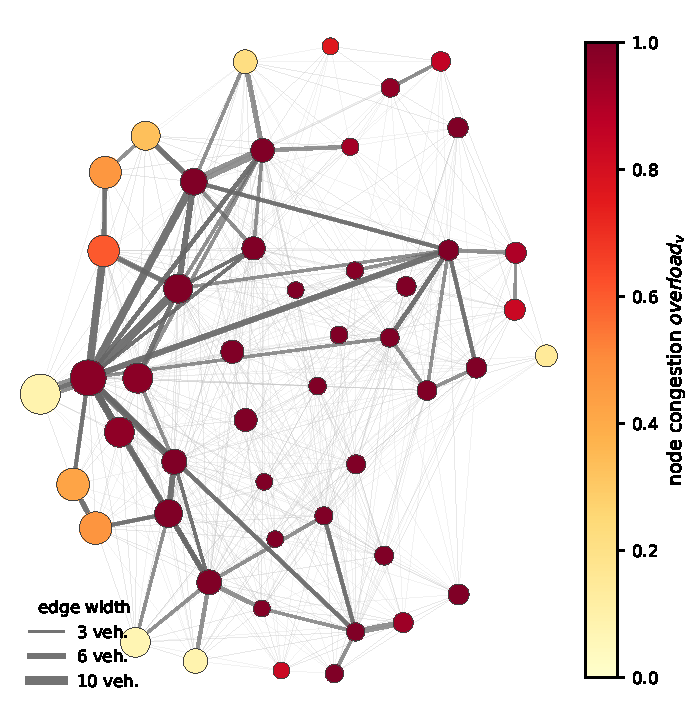
\includegraphics[height=0.46\textheight]{figs/germany_solution.pdf}

{\scriptsize Germany, $|V|=49$: a GVNS solution. Node area $=W_v$, colour $=$
congestion (dark $=$ at capacity), thick edges carry $\ge3$ vehicles.\par
\smallskip
\alert{A MIP solver given two hours returns a solution 54\% more expensive
than this one.}\par}
\end{columns}
\note{Say ``trucks'' and ``reload ceiling'', not ``MCND'' yet; say out loud
that we minimise vehicle movement cost plus reload cost. Point at the map:
thick edges are consolidated backbones, dark nodes are saturated storages. The
54\% is the ratio $1.544$ of Table~2, Germany, MIP-inc.\ column; the exact
budget at this size is 2\,h against a 98\,min limit for GVNS, of which it used
56\,min on average.}
\end{frame}

\begin{frame}{Feature 1: a road is billed per truck, not per unit}
\begin{columns}[T]
\column{0.5\textwidth}
\centering
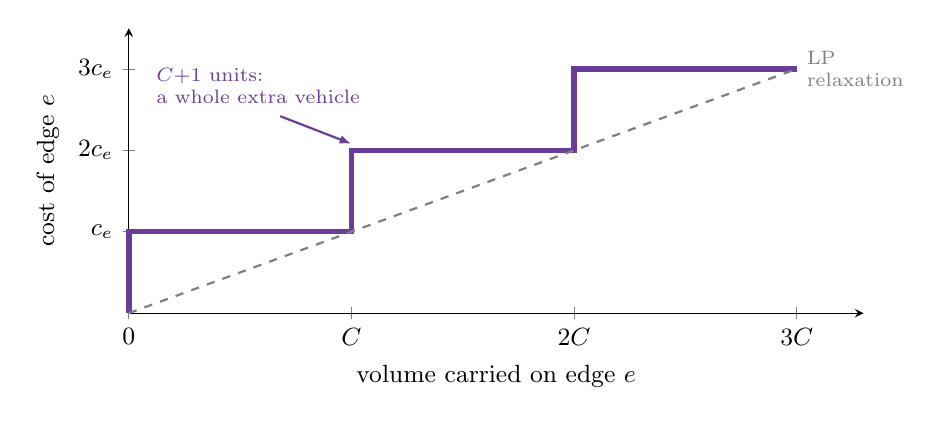
\begin{tikzpicture}
\begin{axis}[width=0.9\linewidth,height=5.2cm,xlabel={volume carried on edge $e$},ylabel={cost of edge $e$},
  xtick={0,50,100,150},xticklabels={0,$C$,$2C$,$3C$},ytick={1,2,3},yticklabels={$c_e$,$2c_e$,$3c_e$},
  ymin=0,ymax=3.5,xmin=0,xmax=165,axis lines=left,clip=false,label style={font=\small},tick label style={font=\small}]
\addplot[const plot mark right,line width=2pt,cStep] coordinates {(0,0)(0.01,1)(50,1)(50.01,2)(100,2)(100.01,3)(150,3)};
\addplot[dashed,gray,thick] coordinates {(0,0)(150,3)} node[pos=1,right,font=\scriptsize,text=gray,align=left] {LP\\relaxation};
\node[font=\scriptsize,text=cStep,align=left,anchor=south west] at (axis cs:4,2.45) {$C{+}1$ units:\\a whole extra vehicle};
\draw[-{Latex[length=1.5mm]},cStep,thick] (axis cs:34,2.42) -- (axis cs:50,2.08);
\end{axis}
\end{tikzpicture}

{\scriptsize schematic, $C=50$}
\column{0.5\textwidth}
\begin{block}{The billed quantity is the vehicle count}
\[
\text{cost of } e = \textcolor{cStep}{c_e\,y_e},\qquad y_e\in\Int_+
\]
with enough vehicles for the flow: $\sum_{k} x^k_e \le C\,y_e$
\end{block}
\begin{itemize}
\item a non-convex \emph{staircase} in the volume, shared by all requests on the edge
\item dropping integrality gives the line $c_e x/C$: the LP relaxation, polynomial but \emph{loose}
\end{itemize}
\end{columns}
\note{Practitioners recognise the staircase instantly; OR people recognise a
step-cost network design problem (Gabrel, Knippel, Minoux 1999; Croxton,
Gendron, Magnanti 2003). How loose: the LP solution with vehicles rounded up,
our starting solution, costs $1.19\times$ the GVNS solution at $|V|=10$,
$2.8\times$ at $|V|=50$ and $2.2$--$3.1\times$ at $|V|\ge90$ (Table~2).}
\end{frame}

\begin{frame}{Feature 2: every storage has a reload ceiling}
\begin{columns}[T]
\column{0.46\textwidth}
\centering
\begin{tikzpicture}[scale=0.72]
  \node[storage,minimum size=13mm,fill=cCap!60,font=\normalsize] (h) at (0,0) {$v$};
  \foreach \a/\c in {150/cN1,180/cN2,210/cOK} {\draw[flow,draw=\c] (\a:2.3) -- (h);}
  \foreach \a/\c in {30/cN1,0/cN2,-30/cOK} {\draw[flow,draw=\c] (h) -- (\a:2.3);}
  \draw[flow,draw=gray,dashed] (-2.4,-1.7) -- (-1.0,-1.0);
  \node[lbl,text=gray,align=left,anchor=north] at (-1.3,-1.85) {no room left:\\this request must detour};
  \draw[thick,mDarkTeal] (2.9,-0.9) rectangle (3.3,0.9);
  \fill[cCap!70] (2.9,-0.9) rectangle (3.3,0.9);
  \node[lbl,right] at (3.4,0.9) {$W_v$};
  \node[lbl,right,align=left] at (3.4,0.1) {transit flow\\$=W_v$};
  \node[lbl,right,text=cCap] at (3.4,-0.75) {$\ovl_v=1.0$};
\end{tikzpicture}

\medskip
{\small congestion of a storage in a solution:\\
$\ovl_v = \text{transit flow through } v\,/\,W_v$\\
$1.0$ = at capacity}
\column{0.54\textwidth}
\begin{block}{Transit volume through $v$ is bounded}
\[
\textcolor{cCap}{\sum_{k\in K:\,v\neq s_k,t_k}\ \sum_{e\in\delta^-(v)} x^k_e \;\le\; W_v}
\qquad\forall v\in V
\]
\end{block}
\begin{itemize}
\item once a storage is at capacity, further transit must detour: a longer route or a reload at a less loaded storage
\item origin and destination handling is not transshipment: a direct $s_k\!\to\!t_k$ route touches no node capacity
\end{itemize}
\end{columns}
\note{Node throughput bounds are familiar from hub location (Alumur \& Kara
2008), not from the MCND literature. $\ovl_v$ returns twice: it colours the
Germany map and it drives neighbourhood $N_3$.}
\end{frame}

\begin{frame}{Why not simply run a published network-design code?}   % [optional]
\centering
\footnotesize
\renewcommand{\arraystretch}{1.15}
\begin{tabular}{@{}l>{\raggedright\arraybackslash}p{4.6cm}>{\raggedright\arraybackslash}p{5.4cm}@{}}
\toprule
 & \textbf{fixed-charge capacitated MCND} & \textbf{this problem}\\
\midrule
arc cost & fixed charge per opened arc $+$ linear flow cost & \textcolor{cStep}{$c_e$ per vehicle: a staircase in the volume}\\
capacities & per arc & per arc (through vehicles) \textbf{and} \textcolor{cCap}{per node: transit volume $\le W_v$}\\
extra cost term & --- & reload $f_v$ per unit at every transit node\\
comparable published code & several (tabu, local branching, matheuristics) & none that we know of\\
\bottomrule
\end{tabular}

\medskip
\begin{alertblock}{Consequence for the experimental design}
no published network-design code that we know of charges per vehicle and bounds node throughput, and our open corpus has no published
objective values: we compare GVNS against \textbf{valid bounds} and \textbf{MIP solvers on the same model}
\end{alertblock}
\note{Skip in a 20-minute slot and say the consequence on the yardstick
slide. Literature, if asked (also on the backup slide ``Where it sits''):
capacitated MCND -- Gendron, Crainic, Frangioni 1999; Crainic 2000; column
generation / branch-and-price -- Barnhart et al.\ 1998; cycle-based tabu --
Ghamlouche, Crainic, Gendreau 2003; local branching -- Rodr\'iguez-Mart\'in \&
Salazar 2010; MILP-in-the-loop matheuristics -- Hewitt, Nemhauser, Savelsbergh
2010; survey -- Crainic \& Gendreau 2021. Step costs -- Gabrel, Knippel,
Minoux 1999; Croxton, Gendron, Magnanti 2003. Node capacity -- hub location,
Alumur \& Kara 2008. VNS -- Mladenovi\'c \& Hansen 1997; Hansen et al.\ 2017;
Hansen \& Mladenovi\'c 2019; multi-start VNS for single-path MCF -- Masri et
al.\ 2015; GVNS on CVRP -- Amous et al.\ 2017. Our own real-life logistic
heuristics: truck-and-trailer routing with time windows and split deliveries
(Batsyn \& Ponomarenko 2014, 2015).}
\end{frame}

% ---------------------------------------------------------------------------
\section{Model}

\begin{frame}{The model: an arc-based MILP}
\small
$x^k_e\in\Real_+$: flow of request $k$ on edge $e$;\quad
$y_e\in\Int_+$: vehicles on $e$;\quad $|K|\cdot|E|+|E|$ variables.
\vspace{-6pt}
\begin{align*}
\min\;& \textcolor{cStep}{\sum_{e\in E} c_e\,y_e}
 \;+\;\sum_{k\in K}\ \sum_{\substack{v\in V\\ v\neq s_k,t_k}}\ \sum_{e\in\delta^-(v)} f_v\,x^k_e
 &&\text{vehicles $+$ reloads}\\[-2pt]
\text{s.t.}\;&
\sum_{e\in\delta^+(v)} x^k_e-\sum_{e\in\delta^-(v)} x^k_e=
 \begin{cases} d_k & v=s_k\\ -d_k & v=t_k\\ 0 & \text{otherwise}\end{cases}
 && \forall k,\ \forall v \quad\text{(demand)}\\[-2pt]
&\textcolor{cStep}{\sum_{k\in K} x^k_e\le C\,y_e} && \forall e\in E \quad\text{(vehicle capacity)}\\
&\textcolor{cCap}{\sum_{k\in K:\,v\neq s_k,t_k}\ \sum_{e\in\delta^-(v)} x^k_e \le W_v} && \forall v\in V \quad\text{(transshipment capacity)}\\
& x\ge 0,\quad y\in\Int_+^{|E|}
\end{align*}
\vspace{-4pt}
linear objective and constraints, integer $y$, continuous $x$: a MILP, NP-hard.
This arc model is exactly what the exact solvers (HiGHS, SCIP) receive later.
\note{Read the equations once; every term was just seen in pictures. The
path-based twin has $\sum_k|\Pi_k|+|E|$ variables. Spoken bridge to the
method if the next frame is skipped: relaxing $y$ gives a per-unit path price,
travel$/C$ plus one reload per transit node, so the relaxation wants cheap
transit-free paths; that is why the start solution is every request on its
direct edge, and why $N_1$ searches with a reload-aware metric.}
\end{frame}

\begin{frame}{Path form, and what the LP relaxation tells us}   % [optional]
\begin{columns}[T]
\column{0.6\textwidth}
\textbf{Path form.} Flow $x^k_p$ on paths $p\in\Pi_k$ (all $s_k\!\to\!t_k$ paths),
$\sum_{p\in\Pi_k}x^k_p=d_k$, same $y_e$; only the paths that carry flow matter.

\medskip
\textbf{Relax integrality.} The capacity constraint becomes tight, so
$y_e=\frac1C\sum_k\sum_{p\ni e}x^k_p$ and $y$ disappears:
\[
\min\ \sum_{k\in K}\sum_{p\in\Pi_k} x^k_p\;
\underbrace{\Bigg(\frac1C\sum_{e\in p} c_e+\sum_{\substack{v\in p\\ v\neq s_k,t_k}} f_v\Bigg)}_{\text{per-unit price of path } p}
\]
\column{0.4\textwidth}
\centering
\begin{tikzpicture}
  \node[storage] (s) at (0,0) {$s$};
  \node[storage,fill=cCap!30] (v) at (2,0.9) {$v$};
  \node[storage] (t) at (4,0) {$t$};
  \draw[flow] (s) -- node[lbl,above left] {$c_{sv}/C$} (v);
  \draw[flow] (v) -- node[lbl,above right] {$c_{vt}/C$} (t);
  \node[lbl,text=cCap,above=1mm of v] {$+\,f_v$};
  \draw[road,dashed] (s) -- node[lbl,below] {$c_{st}/C$, no reload} (t);
\end{tikzpicture}

\medskip
\begin{block}{Reading}
a unit of flow pays \emph{travel}$/C$ plus one reload per transit node: the relaxation prefers cheap, transit-free paths
\end{block}
\end{columns}
\medskip
\begin{itemize}
\item on the completed graph the relaxed optimum puts every request on its direct edge: our \textbf{starting solution}; the search metric of $N_1$ is an edge-wise version of this price
\end{itemize}
\note{Bridge from model to method; skip in a 20-minute slot (the model frame's
note has the spoken version). $N_1$'s metric $c'_{vu}=f_v+f_u+c_{vu}/C$ is
edge-wise, so a transit reload is charged on both incident edges; it is a
ranking metric for path generation, not the objective---the MILP prices every
path exactly.}
\end{frame}

% ---------------------------------------------------------------------------
\section{The GVNS}

\begin{frame}{GVNS at a glance}
\centering
\begin{tikzpicture}[node distance=5mm and 6mm, box/.append style={text width=2.75cm,font=\scriptsize}]
  \node[box] (init) {\textbf{initial solution}\\rounded LP:\\every request on its direct edge};
  \node[box,right=of init,fill=cN2!15] (shake) {\textbf{Shake} in $N_k$\\diversified\\random paths\\MILP budget $\tau_{\mathrm{shk}}$};
  \node[box,right=11mm of shake,fill=cN1!15] (vnd) {\textbf{VND} $N_1\!\to\!N_2\!\to\!N_3$\\restart at $N_1$ on improvement\\MILP budget $\tau_{\mathrm{vnd}}$};
  \node[box,right=of vnd,text width=1.6cm] (test) {$z<z_0$?};
  \draw[road] (init) -- (shake);
  \draw[road] (shake) -- node[lbl,above=2pt,font=\scriptsize] {$z_0\gets z$} (vnd);
  \draw[road] (vnd) -- (test);
  \draw[road,draw=cOK] (test.south) -- ++(0,-0.55) -| node[pos=0.25,below,font=\scriptsize,text=cOK] {yes: $k\gets1$} (shake.south);
  \draw[road,draw=cN3] (test.south) -- ++(0,-1.15) -| node[pos=0.25,below,font=\scriptsize,text=cN3] {no: $k\gets k+1$} ($(shake.south)+(-0.5,0)$);
\end{tikzpicture}

\medskip
\begin{itemize}
\item \textbf{search space: commodity paths.} A solution is a path pool $P$ with flows $x$; vehicle counts follow, $y_e=\big\lceil\frac1C\sum_k x^k_e\big\rceil$
\item \textbf{shake and VND are the same primitive} (next slide): the shake adds more, random paths with a larger MILP budget
\item \textbf{stop} when $k>3$ or after $t_{\max}=2|V|$ minutes; a move is accepted \emph{only if it improves}, so the shake never degrades the incumbent, and $k$ advances when the VND fails to beat the post-shake value $z_0$
\end{itemize}
\note{Preprocessing: complete the graph, build the reload-aware graph $G'$,
precompute 20 shortest paths per request. Shake vs VND path counts: 5 random
pool paths vs 1--3 for $N_1$; stop at 3 fully loaded paths / $5C$ free room vs 2 / $1C$ for $N_2$;
3 detours vs 1 for $N_3$. Budgets: $\tau_{\mathrm{shk}}=10+|V|$ / $100+2|V|$\,s,
$\tau_{\mathrm{vnd}}=25$ / $70$\,s ($N_1$ / rest; 15 / 50\,s at $|V|=100$), so
for $N_1$ the shake budget is smaller than the VND budget while $|V|\le14$.
A VNS-school listener will ask whether this is a shake: it is Algorithm~1
called with diversified generation and $\tau_{\mathrm{shk}}$; diversification
comes from the random paths pushed into the pool and the MILP re-optimisation,
and a non-improving shake is discarded. All parameters are on the backup slide
``Settings''.}
\end{frame}

\begin{frame}{Preprocessing and the starting solution}   % [optional]
\begin{columns}[T]
\column{0.5\textwidth}
\centering
\begin{tikzpicture}[scale=0.68]
  \node[storage] (a) at (0,0) {$a$};
  \node[storage] (b) at (1.6,1.2) {$b$};
  \node[storage] (c) at (3.2,0.2) {$c$};
  \node[storage] (d) at (1.8,-1.2) {$d$};
  \draw[road] (a) -- (b); \draw[road] (b) -- (c); \draw[road] (a) -- (d); \draw[road] (d) -- (c);
  \node[lbl,text=black] at (1.6,-2.0) {(a) raw road graph};
  \begin{scope}[xshift=6.0cm]
  \node[storage] (a2) at (0,0) {$a$};
  \node[storage] (b2) at (1.6,1.2) {$b$};
  \node[storage] (c2) at (3.2,0.2) {$c$};
  \node[storage] (d2) at (1.8,-1.2) {$d$};
  \draw[road] (a2) -- (b2); \draw[road] (b2) -- (c2); \draw[road] (a2) -- (d2); \draw[road] (d2) -- (c2);
  \draw[road,dashed,draw=cN1] (a2) -- node[lbl,text=cN1,above,pos=0.78] {$c_{ac}$} (c2);
  \draw[road,dashed,draw=cN1] (b2) -- (d2);
  \node[lbl,text=black] at (1.6,-2.0) {(b) completed graph};
  \end{scope}
\end{tikzpicture}
\column{0.5\textwidth}
\begin{itemize}
\item road graphs are sparse ($a\!\to\!c$ needs a stop); on the raw graph a missing origin--destination path can even make an instance infeasible
\item \textbf{completion}: join every ordered pair by an edge costing the shortest path in $G$ ($c_{ac}$): the cheapest \emph{stop-free} route, touching no $W_v$
\item the exact solvers get the same completed graph ($|E|=|V|(|V|-1)$)
\end{itemize}
\end{columns}
\smallskip
\begin{block}{Start: the rounded LP}
every request on its direct edge (the relaxed optimum), vehicles rounded up: always feasible, and poor ($1.19\times$ GVNS at $|V|=10$, $2.80\times$ at 50, $3.14\times$ on European Russia)
\end{block}
\note{Skip in a 20-minute slot: say ``we complete the graph so every request
has a direct stop-free edge, and start from the rounded LP''. On the raw graph
the node capacities also shrink the feasible region (paper, Sec.~3.2). Many of the
trucks on those direct edges leave partly empty---that is what $N_2$ will fix.
The initial MILP that sets up the flows has a 300\,s limit.}
\end{frame}

\begin{frame}{The move primitive: propose paths, let the MILP redistribute}
\centering
\begin{tikzpicture}[node distance=5mm]
  \node[box,fill=cN1!10] (gen) {\textbf{GenPaths}$(N,k)$\\new candidate paths $Q$\\for every request $k$};
  \node[box,right=of gen] (milp) {\textbf{MILP} on pool $P\cup Q$\\redistribute flow: warm start $x$,\\time limit $\tau$, gap 1\%};
  \node[box,right=of milp,fill=cOK!10] (keep) {improved ($z'<z$)?\\keep new paths with $x'_p>0$,\\prune every zero-flow path};
  \node[box,below=3mm of keep,fill=cCap!10,text width=3.6cm] (drop) {not improved: discard $Q$};
  \draw[road] (gen) -- (milp);
  \draw[road] (milp) -- (keep);
  \draw[road] (milp.east) -- ++(0.35,0) |- (drop.west);
\end{tikzpicture}

\medskip
\begin{columns}[T]
\column{0.5\textwidth}
\begin{block}{Why paths and not edge flows}
per-edge flows are strongly coupled across requests, so a feasible change needs the whole network at once; a path describes one request only, and \emph{adding} a path to a feasible solution never makes it worse
\end{block}
\column{0.5\textwidth}
\begin{itemize}
\item the three neighbourhoods differ \emph{only} in \textbf{GenPaths}; everything else is shared
\item pruning zero-flow paths keeps the in-loop MILP small enough for budgets of 25--70\,s (VND) and $10{+}|V|$ to $100{+}2|V|$\,s (shake)
\item the neighbourhood proposes, the MILP disposes
\end{itemize}
\end{columns}
\note{This is the matheuristic core; OR people will map it to MILP-in-the-loop
schemes (Hewitt et al.). The MILP is HiGHS with a 1\% gap target.}
\end{frame}

\begin{frame}{\textcolor{cN1}{$N_1$}: reload-aware shortest paths}
\begin{columns}[T]
\column{0.45\textwidth}
\centering
\begin{tikzpicture}[scale=1.15]
  \node[storage] (s) at (0,0) {$s$};
  \node[storage,fill=cCap!30] (h) at (2.2,1.1) {$h$};
  \node[storage] (t) at (4.4,0) {$t$};
  \draw[road,draw=cN1,line width=1.5pt] (s) -- node[lbl,above left,text=cN1] {$c'_{sh}$} (h);
  \draw[road,draw=cN1,line width=1.5pt] (h) -- node[lbl,above right,text=cN1] {$c'_{ht}$} (t);
  \draw[road,draw=cN1,line width=1.5pt] (s) -- node[lbl,below,text=cN1] {$c'_{st}$} (t);
  \foreach \i in {1,...,6} {\draw[cN1!30,line width=0.6pt] (0.2,-0.9-0.13*\i) -- (3.0,-0.9-0.13*\i);}
  \foreach \i in {1,2,3} {\draw[cN1,line width=1pt] (0.2,-0.9-0.13*\i) -- (3.0,-0.9-0.13*\i);}
  \node[lbl,right,text=cN1,align=left] at (3.1,-1.35) {pool of 20 paths\\per request};
\end{tikzpicture}
\column{0.55\textwidth}
\begin{block}{Auxiliary complete graph $G'$: per-unit weights}
\[
c'_{vu}=f_v+f_u+\frac{c_{vu}}{C}\qquad\forall (v,u)\in E
\]
travel per unit plus the reloads at the endpoints; plain shortest paths would ignore the reloads
\end{block}
\begin{itemize}
\item 20 shortest paths per request under $c'$, precomputed once; new paths come from this pool
\item \textbf{VND}: $\{1,2,3\}$ new paths per request $\times$ \{random, low-cost first\}; \textbf{Shake}: 5 random pool paths
\item ablation: without $N_1$, $+0.8\%$ (median, synthetic and real alike)
\end{itemize}
\end{columns}
\note{Keep short: $N_2$ is where the money is. If a sharp listener notes that
$c'$ charges a transit reload on both incident edges and also prices origin
and destination reloads: $c'$ is a ranking metric for path generation, not the
objective; the MILP prices every path exactly, so the double count only changes
which 20 paths enter the pool.}
\end{frame}

\begin{frame}{\textcolor{cN2}{$N_2$}: fill the half-empty trucks}
\begin{columns}[T]
\column{0.46\textwidth}
\centering
\begin{tikzpicture}[x=1cm,y=1cm,scale=0.8]
  \node[font=\footnotesize] at (2.7,1.35) {edge $(u,v)$: 110 units, $y_{uv}=\lceil 110/50\rceil=3$};
  \foreach \i/\l in {0/50, 1/50, 2/10} {
    \draw[thick,mDarkTeal] (\i*1.9,0) rectangle ++(1.6,0.7);
    \fill[cN1!60] (\i*1.9,0) rectangle ++(1.6*\l/50,0.7);
    \node[font=\scriptsize] at (\i*1.9+0.8,-0.3) {\l\,/\,50};
  }
  \draw[{Latex}-{Latex},cN2,line width=1.5pt] (3.8+0.33,0.35) -- (3.8+1.58,0.35);
  \node[font=\scriptsize,text=cN2,align=center] at (4.75,0.95) {40 units free};
  \node[font=\footnotesize,align=center] at (2.7,-1.15) {$\load_{uv}=110 \bmod 50 = 10$:\\up to 40 more units here cost \textbf{no extra vehicle}\\and may free one elsewhere};
\end{tikzpicture}

\medskip
\begin{itemize}
\item shortest paths on $G''$ run through partially loaded vehicles
\item dynamic number of new paths per request: stop after 2 fully loaded paths or accumulated free room $\ge1C$ (VND); 3 fully loaded paths or $\ge5C$ (Shake)
\end{itemize}
\column{0.54\textwidth}
\begin{block}{Graph $G''$ favours free room ($\alpha=0.5$)}
\small
\begin{gather*}
c''_{vu}=f_v+f_u+\frac{\load_{vu}}{C}\Big(\frac{c_{vu}}{C}\Big)^{\!\alpha}\\[-2pt]
\load_e=\Big(\textstyle\sum_k\sum_{p\ni e}x^k_p\Big)\bmod C
\end{gather*}
fully loaded edges ($\load_e=0$) keep their $G'$ weight; smaller residual load $\Rightarrow$ lower weight
\end{block}
\begin{alertblock}{Ablation: the dominant operator}
without $N_2$: $+3.9\%$ synthetic, $+1.6\%$ real (medians), up to $+23.8\%$ on a single instance
\end{alertblock}
\end{columns}
\note{Slow down here. Vehicle consolidation is the main lever on the
objective. On the synthetic ablation subset the mean loss is $+7.1\%$ and the
worst case $+23.8\%$ (50\_nodes\_2); on the real subset the mean is $+2.6\%$
and Germany loses $7.6\%$ (components\_A.csv); none of these is corpus-wide.}
\end{frame}

\begin{frame}{\textcolor{cN3}{$N_3$}: detour around the saturated storage}
\begin{columns}[T]
\column{0.48\textwidth}
\centering
\begin{tikzpicture}
  \node[storage] (a) at (0,0) {$s$};
  \node[storage,minimum size=10mm,fill=cCap!70] (b) at (2.4,0) {$v^\ast$};
  \node[storage] (c) at (4.8,0) {$t$};
  \node[storage,fill=cN1!20] (d) at (2.4,-1.6) {$w$};
  \draw[road] (a) -- (b); \draw[road] (b) -- (c);
  \draw[cCap,line width=1.5pt] (b.north west) -- (b.south east); \draw[cCap,line width=1.5pt] (b.north east) -- (b.south west);
  \draw[flow] (a) to[bend right=25] (d); \draw[flow] (d) to[bend right=25] (c);
  \node[lbl,text=cCap,above=1.5mm of b] {$\ovl_{v^\ast}\approx1$: removed from $G'$};
  \node[lbl,below=1mm of d] {new shortest path through a less loaded $w$};
\end{tikzpicture}

\medskip
{\small in the current solution:\\[2pt]
$\ovl_v=\dfrac1{W_v}\displaystyle\sum_{k:\,v\neq s_k,t_k}\ \sum_{p\in\Pi_k:\,v\in p}x^k_p$}
\column{0.52\textwidth}
\begin{itemize}
\item delete the \textbf{single most congested} storage from $G'$ (unless it is the request's own origin or destination), recompute the shortest path: a detour to less loaded storages
\item 1 new path per request in VND, 3 in Shake
\item ablation: $+0.1\%$ / $+0.2\%$ median, \textbf{inactive when capacities are slack}; $+4.0\%$ on Germany, where almost every storage runs at capacity
\end{itemize}
\end{columns}
\note{Say ``situational'' out loud: the operator is worth carrying only for
tight instances---when capacities are slack there is nothing to route around.
Point back at the Germany map. If asked why a single node: removing a prefix
of $|V|/5$--$|V|/4$ congested storages was tried on all 50 instances $\times$
10 seeds; it is indistinguishable on 44 of 50 (within across-seed noise) yet
forfeits $N_3$'s benefit on the capacity-tight networks, so the surgical
version is kept---state the measured outcome, not a mechanism.}
\end{frame}

% ---------------------------------------------------------------------------
\section{Experiments}

\begin{frame}{The benchmark: realistic regional networks, openly available}
\begin{columns}[T]
\column{0.56\textwidth}
\begin{itemize}
\item our open corpus (arXiv:2606.20653; Zenodo, CC-BY-4.0), every instance reproducible from its published seed
\item road networks between regional sorting centres, calibrated on OpenStreetMap for \textbf{nine European countries, five U.S.\ states and European Russia}
\item real structure: Zipf city sizes, spatial-network topology, centrality-driven $W_v$, gravity demand; near-planar, large-diameter graphs
\item \textbf{35 synthetic}: $10\times|V|{=}10$, $7\times20$, $7\times30$, $5\times50$, $3\times100$, $3\times150$
\item \textbf{15 real-geometry}: Denmark ($|V|=11$) to European Russia ($|V|=90$)
\end{itemize}
\column{0.44\textwidth}
\centering
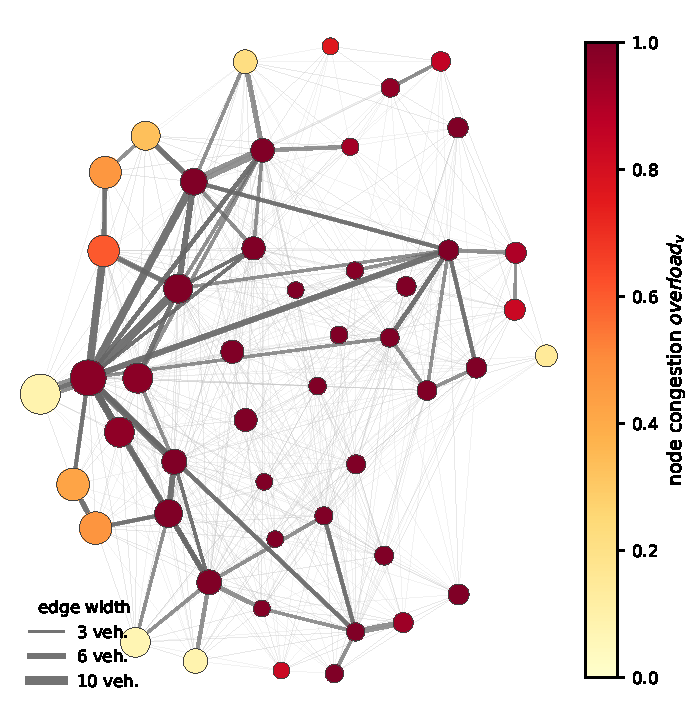
\includegraphics[height=0.52\textheight]{figs/germany_solution.pdf}

{\scriptsize Germany ($|V|=49$), the solution from the first slide:
almost every storage runs at capacity.\par}
\end{columns}
\note{The generator is a separate paper; here only what the study needs.
Mean degree is 3.575 in the paper. Point at the map: thick edges are
consolidation ($N_2$) made visible, dark nodes are what $N_3$ works on. The
instance's numbers come where they are defined: $\gapLB=11.0\%$, exact
incumbent $1.544\times$, rounded-LP start $2.692\times$, $\sigma$ over 10 seeds
$2.0\%$; without $N_2$ $+7.6\%$, without $N_3$ $+4.0\%$.}
\end{frame}

\begin{frame}{Setup and yardsticks}
\centering
\begin{tikzpicture}[x=1cm]
  \draw[-{Latex[length=2.5mm]},thick,mDarkTeal] (0,0) -- (13.2,0) node[right,font=\scriptsize] {objective};
  \foreach \x/\lab/\val/\col in {0.9/{LP relaxation}/{0.971}/gray, 3.6/{MIP dual bound $\underline{z}$}/{}/cN1, 6.2/{optimum $z^\ast$}/{(unknown)}/gray, 8.8/{GVNS}/{1.0}/mLightBrown, 11.8/{rounded LP (start)}/{1.192}/gray}{
    \draw[thick,\col] (\x,-0.15) -- (\x,0.15);
    \node[font=\scriptsize,text=\col,align=center,above=1mm] at (\x,0.15) {\lab\\ \val};
  }
  \node[font=\scriptsize,text=cOK,align=center,below=1mm] at (8.8,-0.15) {MIP incumbent 1.000};
  \draw[{Bar}-{Bar},thick,cN1] (3.6,-0.75) -- (8.8,-0.75) node[midway,below,font=\scriptsize,text=cN1] {$\gapLB=0.96\%$};
  \node[font=\scriptsize,text=gray] at (11.8,-0.8) {ratios: means at $|V|=10$; not to scale};
\end{tikzpicture}

\smallskip
\begin{columns}[T]
\column{0.48\textwidth}
\begin{block}{Two metrics}
\small
$\gapLB=\big(\mathit{Result}_{\mathrm{GVNS}}-\underline{z}\big)/\underline{z}$,\quad $\underline{z}=$ best MIP dual bound:
an \textbf{upper bound on the true optimality gap} of GVNS\\[3pt]
$\mathit{Ratio}_{\mathrm{method}}=\mathit{Result}_{\mathrm{method}}/\mathit{Result}_{\mathrm{GVNS}}$:
below 1 better than GVNS, above 1 worse
\end{block}
\column{0.52\textwidth}
\begin{itemize}\small
\item GVNS: 10 seeds per instance, limit $2|V|$\,min; exact: gap target 0, 30\,min--4\,h, i.e.\ comparable budgets ($|V|=50$: 100\,min vs 2\,h); HiGHS is the exact baseline \emph{and} the in-loop solver
\item nothing is proven optimal, but $\underline{z}$ is a valid lower bound, typically within a few percent of the incumbent: $\gapLB$ is a guarantee, not a self-comparison
\end{itemize}
\end{columns}
\note{Hardware: HSE cluster cHARISMa, nodes with 2$\times$AMD EPYC (44 cores,
$\ge$720\,GB RAM), each job pinned to 8 cores; HiGHS 1.14.0, SCIP 10.0.2 as
cross-check. Exact side in one breath: none of the 50 instances was solved to
proven optimality; up to $|V|=42$ the two solvers' dual bounds agree within
$0.6\%$; SCIP returns nothing usable from $|V|=45$; the arc model is out of
memory at $|V|\ge100$ (backup ``The exact side''). If you accept one number
from this talk, make it $\gapLB$: it bounds the distance to the optimum instead
of comparing GVNS with itself. The ladder ticks are the $|V|=10$ means of
Table~2; the dual bound sits between the LP and GVNS, and GVNS is $0.96\%$
above it.}
\end{frame}

\begin{frame}{Results I: synthetic instances}
\begin{columns}[T]
\column{0.56\textwidth}
\centering
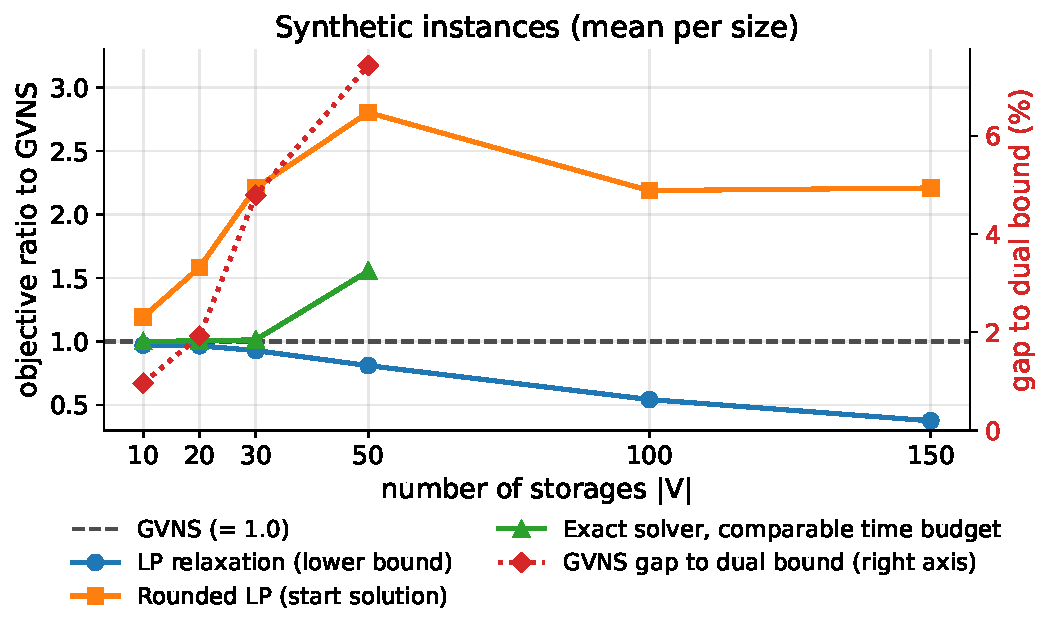
\includegraphics[width=0.94\linewidth]{figs/ratios_synthetic.pdf}
\column{0.44\textwidth}
\centering
\small
\setlength{\tabcolsep}{4pt}
\begin{tabular}{@{}rrccc@{}}
\toprule
$|V|$ & $n$ & $\gapLB$ & exact inc. & $\sigma$\\
\midrule
10  & 10 & 0.96\% & 1.000 & 0.06\%\\
20  & 7  & 1.92\% & 1.005 & 0.18\%\\
30  & 7  & 4.79\% & 1.013 & 0.68\%\\
50  & 5  & 7.44\% & \alert{1.555} & 0.66\%\\
100 & 3  & \dag & \dag & 0.31\%\\
150 & 3  & \dag & \dag & 0.38\%\\
\bottomrule
\end{tabular}

{\scriptsize\dag: arc model intractable; only the loose LP bound (0.542, 0.375)\par}

\smallskip
{\small near-optimal up to $|V|=20$; at $|V|=50$ the exact solver with a comparable budget is \alert{55\% more expensive} on average (16\% to 137\% per instance)\par}
\end{columns}
{\scriptsize GVNS mostly stops before its limit (3\,729 of 6\,000\,s at $|V|=50$); the exact solver always used its full budget, so the comparison is conservative.\par}
\note{Trace the green curve: flat at 1.0, up to 1.555 at 50, then it stops
existing. Spoken: $\gapLB$ is about 1--2\% up to $|V|\approx20$, 4.8\% at 30,
7.4\% at 50, where the LP bound alone would say about 24\%; at $|V|\ge100$
GVNS still ends $2.2\times$ below its own start. Mean run time vs limit:
633/1\,200\,s (10), 1\,952/2\,400 (20), 2\,611/3\,600 (30), 3\,729/6\,000 (50),
5\,983/12\,000 (100), 18\,236/18\,000 (150); the 150-node mean slightly exceeds
its limit because Algorithm~2 tests $t_{\max}$ only before each shake and after
each full VND sweep, so a shake started just under the limit (MILP budget up to
$100+2|V|=400$\,s at $|V|=150$) and the sweep after it run to completion.
Per-instance $|V|=50$ numbers are on the backup slide ``What the means hide''.}
\end{frame}

\begin{frame}{Results II: real road geometries mirror the synthetic story}
\begin{columns}[T]
\column{0.58\textwidth}
\centering
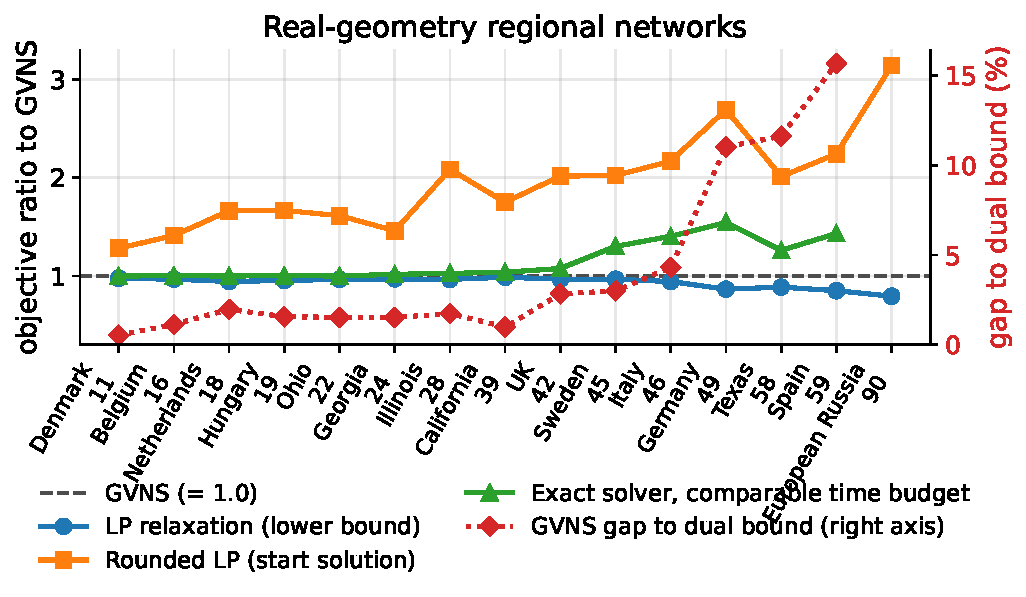
\includegraphics[width=\linewidth]{figs/ratios_real.pdf}
\column{0.42\textwidth}
\begin{itemize}
\item exact solver with a comparable budget: parity up to $|V|=22$, $1.02$--$1.08\times$ up to the UK (42), then \alert{$1.26$--$1.54\times$} from Sweden (45) to Spain (59)
\item $\gapLB$ from $0.5\%$ (Denmark, 11) to $15.7\%$ (Spain, 59)
\item European Russia ($|V|=90$): no exact reference; GVNS ends $3.1\times$ below its start
\end{itemize}
\medskip
{\small\itshape same shape as the synthetic curves: the synthetic corpus behaves like the real geometries, and GVNS is robust to them}
\end{columns}
\note{Do not read the table; point at the three medium networks and at the
90-node one. Spoken detail: $\gapLB$ about 1--3\% up to $|V|=45$, 4.3\% on
Italy (46), 11.0\% Germany (49), 11.6\% Texas (58), 15.7\% Spain (59); exact
incumbent 1.02--1.04$\times$ from Georgia (24) to California (39), 1.077 UK;
run time 615\,s (Denmark) to 3\,986\,s (Spain), 5\,595\,s on European Russia.
Full Table~2 rows are in the paper.}
\end{frame}

\begin{frame}{How many seeds do you need?}   % [optional]
\begin{columns}[T]
\column{0.58\textwidth}
\centering
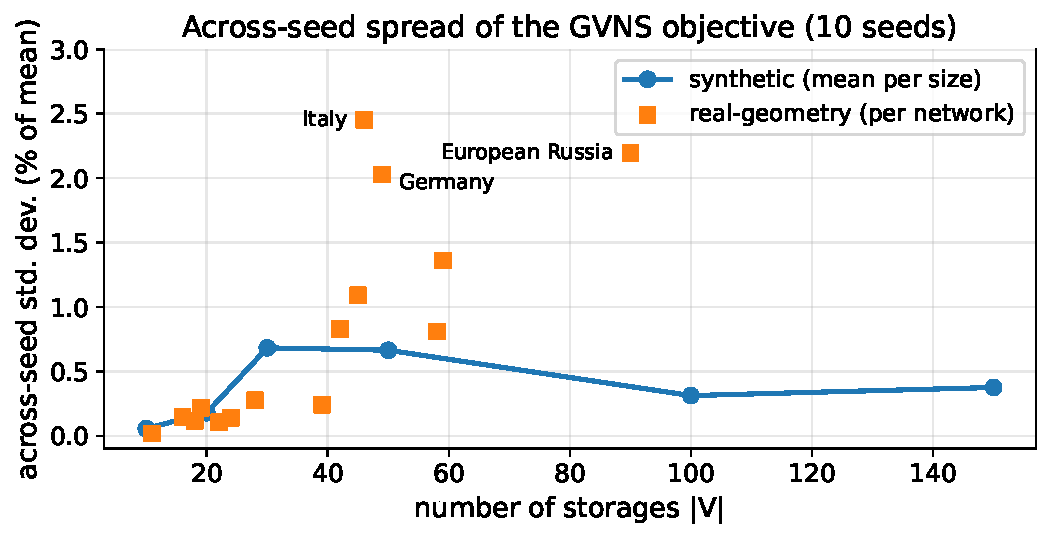
\includegraphics[width=\linewidth]{figs/seed_spread.pdf}
\column{0.42\textwidth}
\begin{itemize}
\item synthetic: across-seed $\sigma$ below $0.7\%$ of the mean at every size, below $0.2\%$ up to $|V|=20$
\item large real networks: $2.0\%$ (Germany), $2.5\%$ (Italy), $2.2\%$ (European Russia)
\item \alert{three seeds badly understate it}: on Italy the spread over three seeds is $0.4\%$ against $2.5\%$ over ten
\item one run is representative on small networks; on capacity-tight instances take the best of several
\end{itemize}
\end{columns}
\note{Backup for the ``is it stable?'' question. We moved from 3 to 10 seeds
for the headline numbers and 5 for the component study.}
\end{frame}

\begin{frame}{What each component buys}
\begin{columns}[T]
\column{0.54\textwidth}
\centering
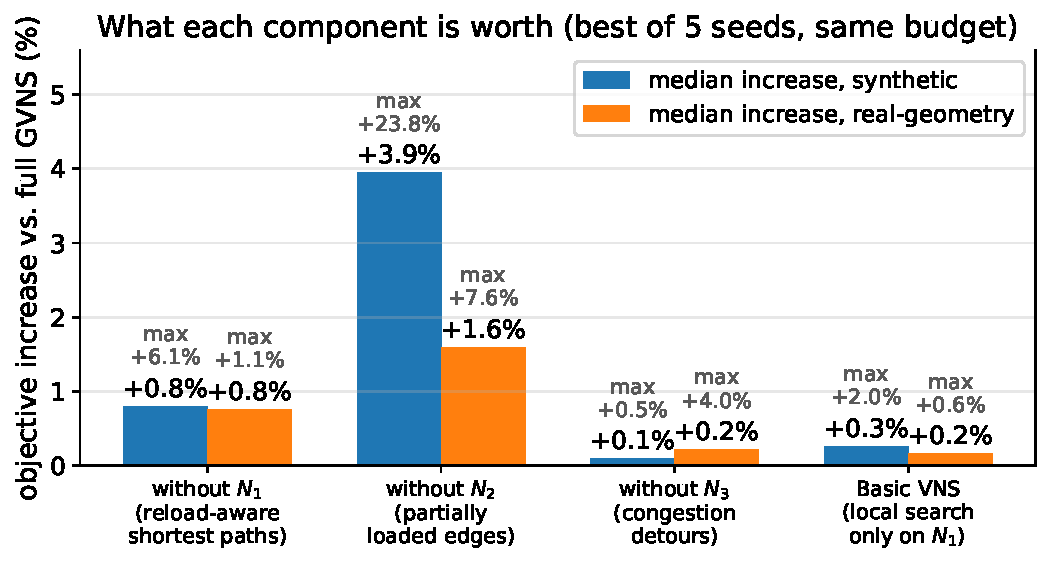
\includegraphics[width=\linewidth]{figs/ablation.pdf}

{\scriptsize best of 5 seeds, same budget, subset of synthetic ($|V|=20$--$100$) and real ($16$--$49$) instances; medians because the seed spread is heavy-tailed on capacity-tight networks\par}
\column{0.46\textwidth}
\footnotesize
\setlength{\tabcolsep}{3pt}
\begin{tabular}{@{}lcc@{}}
\toprule
GVNS better / tie / variant better & synth. & real\\
\midrule
without $N_1$ & 8 / 0 / 1 & 5 / 1 / 0\\
without $N_2$ & 8 / 1 / 0 & 5 / 1 / 0\\
without $N_3$ & 1 / 8 / 0 & 3 / 3 / 0\\
Basic VNS & 5 / 4 / 1 & 2 / 4 / 0\\
\bottomrule
\end{tabular}

{\scriptsize ``decided'' = difference beyond the seed spread of both runs; time relative to GVNS: 0.80, 0.52, 0.68, 0.63\par}

\medskip
\begin{itemize}\small
\item \textcolor{cN2}{$N_2$ dominates}; \textcolor{cN3}{$N_3$ is situational}: ties when capacities are slack, $+4.0\%$ on Germany
\item \textbf{Basic VNS} (local search on $N_1$ only, same shake): GVNS better on 7 of 16, Basic VNS on 1, 8 ties; the margin grows with size, $0.2$--$0.6\%$ at $|V|\le28$ vs $1.1$--$2.0\%$ at $|V|\ge50$, for $1/0.63$ of the time
\end{itemize}
\end{columns}
\note{One line: $N_2$ dominates, the VND matters at scale, $N_3$ is for tight
instances. Table~3's time ratios are the means of the synthetic and real
groups (CSV: $N_1$ 0.76/0.84, $N_2$ 0.54/0.50, $N_3$ 0.73/0.63, Basic VNS
0.68/0.58). The CSV's \texttt{argmax\_instance} names the instance where the
variant is \emph{worst}, not best. Single instances can flip sign: the two
``variant better'' entries in the table are decided (beyond the seed spread of
both runs): 50\_nodes\_2, where dropping $N_1$ improved the result by 2.1\%, and
30\_nodes\_2, where Basic VNS beat GVNS by 1.3\%; Basic VNS also improves
Germany by 4.0\%, but inside its 4.2\% seed spread there, so a tie.}
\end{frame}

% ---------------------------------------------------------------------------
\section{Closing}

\begin{frame}{Limitations, and what comes next}
\begin{columns}[T]
\column{0.5\textwidth}
\textbf{Stated before you ask}
\begin{itemize}\small
\item \textbf{static capacities and costs}: on real networks they vary with the time of day
\item \textbf{no proven optima}: $\gapLB$ is an upper bound on the true gap
\item \textbf{no tight reference beyond $|V|=59$}: only the loose LP bound
\item \textbf{path generation is heuristic}: a pool of 20 shortest paths plus three rules
\item \textbf{open-source solvers at default settings} as the exact baseline (tuning checked on 8 instances)
\item \textbf{component study} on a subset with five seeds; \textbf{no operational data} yet
\end{itemize}
\column{0.5\textwidth}
\textbf{Next}
\begin{itemize}\small
\item time-expanded graph with period-dependent $C_e(t)$, $W_v(t)$: the neighbourhoods only need a period-aware edge metric
\item column-generation pricing to feed the path pool
\item validation on operational data
\end{itemize}
\end{columns}
\note{Justifications, spoken: at $|V|=50$--$59$ the 7--16\% gap cannot be split
between heuristic error and bound weakness; beyond $|V|=59$ the LP bound is
0.795 on European Russia and 0.542 / 0.375 at 100 / 150; HiGHS and SCIP with
three presets each moved nothing (backup ``The exact side''). The ``next''
items answer the first, fourth and last limitations.}
\end{frame}

\begin{frame}{Takeaways}
\begin{enumerate}\setlength{\itemsep}{8pt}
\item \textcolor{cStep}{integer trucks} $+$ \textcolor{cCap}{reload ceilings}: compare against \textbf{valid dual bounds}, not fixed-charge codes
\item path-space GVNS: within $\approx1\%$ of the dual bound on small networks; the exact solver is \textbf{up to 55\% more expensive} at $|V|=50$
\item \textcolor{cN2}{$N_2$} is the lever, \textcolor{cN3}{$N_3$} only when capacity binds, the full VND pays at scale
\end{enumerate}
\bigskip
\begin{center}
{\large\itshape Let cheap path generators propose and a time-boxed MILP dispose:\\
$N_2$ always, $N_3$ when capacity binds, the full VND once the network is large.}
\end{center}
\note{End on the italic sentence; it calls back to ``the neighbourhood
proposes, the MILP disposes'' on the primitive slide.}
\end{frame}

\begin{frame}{Thank you}
\begin{columns}[T]
\column{0.58\textwidth}
\textbf{Code, exact-solver harness, scripts that regenerate every table and figure}\\
{\small\href{https://github.com/aponom84/Optimal-Logistic-Net}{\texttt{github.com/aponom84/Optimal-Logistic-Net}}}

\medskip
\textbf{Instance corpus} (CC-BY-4.0)\\
{\small\href{https://doi.org/10.5281/zenodo.20372456}{\texttt{doi.org/10.5281/zenodo.20372456}}}

\medskip
\textbf{Contact}\\
\texttt{aponomarenko@hse.ru} $\cdot$ \texttt{varvara\_kovaleva03@mail.ru}

\bigskip
{\footnotesize Supported by the Basic Research Program at HSE University
(HSE-BR-2025-080) and by the HPC facilities of HSE University (cHARISMa).\par}
\column{0.42\textwidth}
\centering
\begin{tabular}{c@{\hspace{6mm}}c}
\qrcode[height=2.4cm]{https://github.com/aponom84/Optimal-Logistic-Net} &
\qrcode[height=2.4cm]{https://doi.org/10.5281/zenodo.20372456}\\[3pt]
{\small code} & {\small data}
\end{tabular}
\end{columns}
\note{Question map: seeds -- ``How many seeds''; solver behaviour and tuning --
backup ``The exact side''; per-instance spread at $|V|=50$ -- backup ``What
the means hide''; any parameter -- backup ``Settings''; literature -- backup
``Where it sits''; the $N_3$ prefix variant -- the $N_3$ slide's note.}
\end{frame}

% ---------------------------------------------------------------------------
% Backup slides: no progress bar (its denominator is the appendix frame
% count, which appendixnumberbeamer only knows after the first pass).
\appendix
\metroset{progressbar=none}

\begin{frame}{Backup: settings (Table~1 of the paper)}
\centering
\small
\renewcommand{\arraystretch}{1.15}
\setlength{\tabcolsep}{4pt}
\begin{tabular}{llll}
\toprule
Setting & Value & Setting & Value\\
\midrule
neighbourhoods $k_{\max}$ & 3 & $N_2$ exponent $\alpha$ & 0.5\\
GVNS limit $t_{\max}$ & $2|V|$\,min & $N_2$ free-room stop & $1C$ / $5C$\\
random seeds & 10 / 5 (components) & $N_3$ storages removed & 1 (most congested)\\
vehicle capacity $C$ & 50 & $N_1$ path pool & 20\\
$N_1$ paths per request & 1--3 / 5 & $N_3$ paths per request & 1 / 3\\
initial MILP limit & 300\,s & exact gap target & 0\\
redistribution MILP gap & 1\% & exact budget & 30\,min--4\,h\\
$\tau_{\mathrm{shk}}$ ($N_1$ / rest) & $10{+}|V|$ / $100{+}2|V|$\,s & $\tau_{\mathrm{vnd}}$ ($N_1$ / rest) & 25 / 70\,s ($15$ / $50$\,s at $|V|=100$)\\
\bottomrule
\end{tabular}

\medskip
{\footnotesize Values given as VND / Shake where they differ. Each job pinned to 8 cores;
HSE cluster cHARISMa (2$\times$AMD EPYC, 44 cores, $\ge$720\,GB RAM per node); HiGHS 1.14.0, SCIP 10.0.2.}
\end{frame}

\begin{frame}{Backup: the exact side, and is the baseline understated?}
\centering
\scriptsize
\renewcommand{\arraystretch}{1.05}
\begin{tabular}{@{}l>{\raggedright\arraybackslash}p{4.2cm}>{\raggedright\arraybackslash}p{4.6cm}>{\raggedright\arraybackslash}p{3.2cm}@{}}
\toprule
 & \textbf{HiGHS 1.14} & \textbf{SCIP 10} & \textbf{arc MILP size}\\
\midrule
$|V|\le 42$ & dual bound $+$ incumbent & dual bound agrees with HiGHS within $0.6\%$ (mean $0.18\%$); weaker incumbent & $\approx6\,000$ variables at $|V|=10$\\
$|V|=45$--$59$ & dual bound $+$ incumbent & \textcolor{cCap}{no feasible solution, no non-trivial bound} & \\
$|V|\ge 90$ & \multicolumn{2}{>{\raggedright\arraybackslash}p{9cm}}{millions of variables: at $|V|=90$ only SCIP was tried and returns no bound and no incumbent; \textcolor{cCap}{out of memory} for both at $|V|\ge100$} & $3.7\times10^{8}$ at $|V|=150$\\
\bottomrule
\end{tabular}

\smallskip
\begin{columns}[T]
\column{0.5\textwidth}
\scriptsize
budgets: MIP-gap target 0, 30\,min ($|V|=10$) to 4\,h ($|V|=150$); \alert{none of the 50 instances solved to proven optimality}, but the branch-and-bound dual bound is tight and well above the LP.

\smallskip
\textbf{Tuning check}: 8 instances ($|V|=30$--$59$), three non-default presets per backend (HiGHS: aggressive heuristics, presolve off, full parallelism; SCIP: aggressive heuristics, feasibility emphasis, aggressive separation). SCIP: no preset helps; two presets \emph{degrade} the dual bound by up to $2.3\%$ and the incumbent by up to $48\%$; on the six subset instances with $|V|\ge45$ no preset finds a feasible solution.

\smallskip
\alert{\textbf{The default configuration does not understate the exact baseline.}}
\column{0.5\textwidth}
\centering
\scriptsize
\setlength{\tabcolsep}{4pt}
\begin{tabular}{@{}lrr@{}}
\toprule
instance & \multicolumn{2}{c}{HiGHS, column-wise best of 3 presets vs default}\\
 & dual bound & incumbent\\
\midrule
30\_nodes\_1 & $+0.005\%$ & $+0.054\%$\\
30\_nodes\_2 & $+0.015\%$ & $0$\\
50\_nodes\_1 & $+0.002\%$ & $+0.285\%$\\
50\_nodes\_2 & $0$ & $0$\\
Sweden (45) & $+0.003\%$ & $+0.823\%$\\
Germany (49) & $+0.023\%$ & $+0.108\%$\\
Texas (58) & $+0.036\%$ & $+0.454\%$\\
Spain (59) & $+0.029\%$ & $+0.885\%$\\
\bottomrule
\end{tabular}

{\scriptsize $+$ = improvement; full grid in \texttt{Results/exact\_tuning.csv}\par}
\end{columns}
\note{HiGHS is the stronger exact solver here and therefore also the in-loop
solver of GVNS. Europe Russia ($|V|=90$) was attempted with SCIP only (time
limit, no bound, no incumbent); the paper reports the arc model as intractable
from about $|V|=90$ and out of memory at $|V|\ge100$.}
\end{frame}

\begin{frame}{Backup: what the means hide at $|V|=50$}
\centering
\small
\setlength{\tabcolsep}{6pt}
\begin{tabular}{@{}lccccr@{}}
\toprule
instance & $\gapLB$ & exact inc. & rounded LP & LP relax. & mean GVNS time\\
\midrule
50\_nodes\_1 & 2.99\% & 1.162 & 2.151 & 0.827 & 2\,890\,s\\
50\_nodes\_2 & \alert{14.61\%} & \alert{2.368} & 4.131 & 0.777 & 5\,583\,s\\
50\_nodes\_3 & 5.25\% & 1.410 & 2.707 & 0.784 & 4\,001\,s\\
50\_nodes\_4 & 9.69\% & 1.523 & 2.668 & 0.854 & 2\,954\,s\\
50\_nodes\_5 & 4.64\% & 1.311 & 2.363 & 0.805 & 3\,215\,s\\
\midrule
mean & 7.44\% & 1.555 & 2.804 & 0.810 & 3\,729\,s\\
\bottomrule
\end{tabular}

\medskip
\begin{itemize}
\item $50\_nodes\_2$ is where the exact solver falls furthest behind of any instance with a dual bound: its incumbent is $2.37\times$ GVNS, the rounded-LP start $4.13\times$; only Spain ($|V|=59$, $15.7\%$) has a larger $\gapLB$
\item on this instance the $14.6\%$ cannot be split between heuristic error and bound weakness; the LP bound alone would put the gap at $29\%$, so the dual bound is already much tighter
\item per-instance $\gapLB$ at the smaller sizes: $0.38$--$1.95\%$ at $|V|=10$, $1.08$--$2.66\%$ at 20, $2.42$--$6.58\%$ at 30
\end{itemize}
\end{frame}

\begin{frame}{Backup: where it sits in the literature}
\begin{columns}[T]
\column{0.5\textwidth}
\textbf{Capacitated multicommodity network design}
\begin{itemize}\scriptsize
\item Gendron, Crainic, Frangioni (1999); Crainic (2000): fixed-charge MCND, NP-hard
\item Barnhart et al.\ (1998): branch-and-price on path formulations
\item Ghamlouche, Crainic, Gendreau (2003): cycle-based tabu search
\item Rodr\'iguez-Mart\'in, Salazar-Gonz\'alez (2010): local branching
\item Hewitt, Nemhauser, Savelsbergh (2010): MILP-in-the-loop matheuristics
\item Crainic, Gendreau (2021): survey of (meta)heuristics
\end{itemize}
\textbf{Step costs and node capacities}
\begin{itemize}\scriptsize
\item Gabrel, Knippel, Minoux (1999): exact Benders-type method for general step costs
\item Croxton, Gendron, Magnanti (2003): MILP models of nonconvex piecewise-linear costs
\item Alumur, Kara (2008): hub location with bounded hub throughput
\end{itemize}
\column{0.5\textwidth}
\textbf{Variable neighbourhood search}
\begin{itemize}\scriptsize
\item Mladenovi\'c, Hansen (1997); Hansen et al.\ (2017); Hansen, Mladenovi\'c (2019): VNS, GVNS
\item Karakostas et al.\ (2019); Mjirda et al.\ (2016): GVNS vs single-neighbourhood schemes
\item Masri, Krichen, Guitouni (2015): multi-start VNS for the single-path multicommodity flow problem
\item Amous et al.\ (2017): VNS for the capacitated VRP
\end{itemize}
\textbf{Real-life logistic routing}
\begin{itemize}\scriptsize
\item Batsyn, Ponomarenko (2014, 2015): truck-and-trailer routing with time windows and split deliveries
\end{itemize}
\textbf{Benchmark}
\begin{itemize}\scriptsize
\item Kovaleva, Ponomarenko (2026): generator and corpus, arXiv:2606.20653, Zenodo 10.5281/zenodo.20372456
\end{itemize}
\end{columns}
\end{frame}

\end{document}
"
% to get the speaker-notes version (see build.sh)
\ifdefined\shownotes
  \setbeameroption{show notes on second screen=right}
\fi

% Colour system carried through the talk:
%   cStep -- feature 1, per-vehicle step cost      cCap -- feature 2, reload ceiling
%   cN1 / cN2 / cN3 -- the three neighbourhoods    (cN3 = cCap: N3 acts on congestion)
\definecolor{cStep}{HTML}{6A3D9A}
\definecolor{cCap}{HTML}{B2182B}
\definecolor{cN1}{HTML}{1F77B4}
\definecolor{cN2}{HTML}{E8710A}
\definecolor{cN3}{HTML}{B2182B}
\definecolor{cOK}{HTML}{2E7D32}

\tikzset{
  storage/.style={circle,draw=mDarkTeal,thick,fill=mDarkTeal!10,minimum size=7mm,inner sep=0pt,font=\small},
  road/.style={-{Latex[length=2mm]},draw=mDarkTeal!60,thick},
  flow/.style={-{Latex[length=2.5mm]},draw=mLightBrown,line width=2pt},
  box/.style={draw=mDarkTeal,thick,rounded corners=2pt,fill=mDarkTeal!5,align=center,font=\small,inner sep=5pt,minimum height=9mm},
  lbl/.style={font=\scriptsize,text=mDarkTeal!80},
  truck/.pic={\draw[fill=white,thick] (-0.28,0) rectangle (0.18,0.22);
              \draw[fill=white,thick] (0.18,0) rectangle (0.32,0.15);
              \fill (-0.18,0) circle(0.045); \fill (0.2,0) circle(0.045);},
}

\newcommand{\Real}{\mathbb{R}}
\newcommand{\Int}{\mathbb{Z}}
\newcommand{\gapLB}{gap_{\mathrm{LB}}}
\newcommand{\ovl}{\mathit{overload}}
\newcommand{\load}{\mathit{load}}
\setlength{\leftmargini}{1.2em}
\setbeamersize{text margin left=0.7cm,text margin right=0.7cm}

\title{A General Variable Neighborhood Search for Logistic Network Flow Design
  with Nonlinear Edge Costs and Transshipment Capacities}
\subtitle{OPTIMA 2026}
\author{Varvara Kovaleva\inst{1} \and Alexander Ponomarenko\inst{2}}
\institute{\inst{1} HSE University, Nizhny Novgorod \and
  \inst{2} Laboratory of Algorithms and Technologies for Network Analysis, HSE University, Nizhny Novgorod}
\date{}

\begin{document}

\maketitle
\note{One breath, then the hook: ``Every night, freight between regional sorting
centres moves in trucks that are either full or not, and every centre can only
reload so much. Those two facts alone break the textbook flow model---this talk
is about what to do instead.''}

% ---------------------------------------------------------------------------
\section{The problem}

\begin{frame}{Freight between regional sorting centres}
\begin{columns}[T]
\column{0.56\textwidth}
\centering
\begin{tikzpicture}[scale=0.82]
  \node[storage,minimum size=8mm] (s) at (0,0) {$s_k$};
  \node[storage,minimum size=11mm,fill=cCap!35] (u) at (2.6,1.5) {$u$};
  \node[storage,minimum size=6mm] (w) at (2.6,-1.2) {$w$};
  \node[storage,minimum size=9mm] (t) at (5.2,0) {$t_k$};
  \draw[road] (s) -- node[lbl,below right,pos=0.55] {$c_{su}$} (u);
  \draw[road] (u) -- node[lbl,below left,pos=0.45] {$c_{ut}$} (t);
  \draw[road] (s) -- node[lbl,below left] {$c_{sw}$} (w);
  \draw[road] (w) -- node[lbl,below right] {$c_{wt}$} (t);
  \draw[road] (s) -- node[lbl,below,pos=0.6] {$c_{st}$ (direct)} (t);
  \draw[flow,opacity=0.85] (s) to[bend left=18] (u);
  \draw[flow,opacity=0.85] (u) to[bend left=18] (t);
  \pic at (1.0,1.15) {truck};
  \node[lbl,text=mLightBrown] at (0.75,1.65) {$C$ units};
  \node[lbl,text=cCap,above=1mm of u,align=center] {reload $f_u$ per unit; at most $W_u$ in transit};
  \node[lbl,left=1mm of s] {demand $d_k$};
\end{tikzpicture}

\medskip
\begin{itemize}\setlength{\itemsep}{2pt}
\item \textbf{storages} $v$: reload cost $f_v$ per unit, \textcolor{cCap}{transshipment capacity $W_v$}
\item \textbf{roads} $e$: cost $c_e$ \textcolor{cStep}{per vehicle}; a vehicle carries $C$ units ($C=50$)
\item \textbf{requests} $k$: ship $d_k$ units from $s_k$ to $t_k$, reloading on the way if useful
\end{itemize}
\column{0.44\textwidth}
\centering
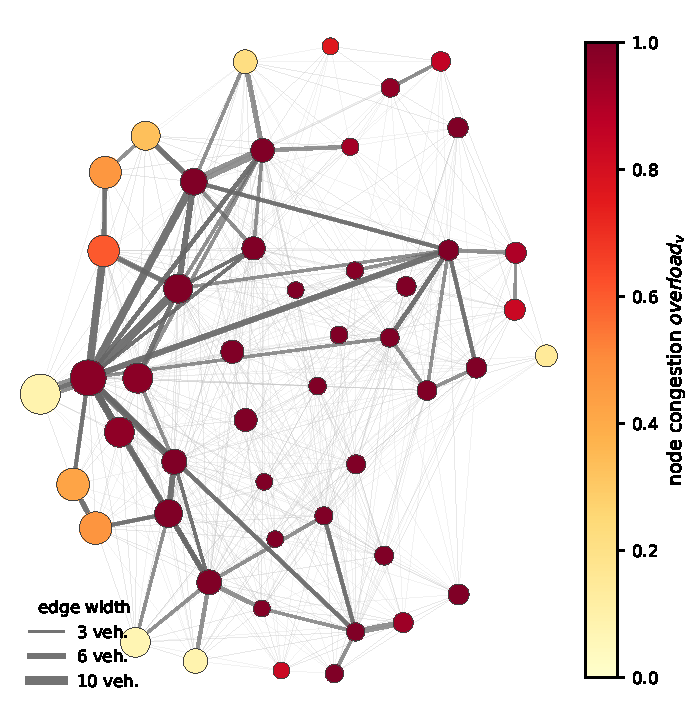
\includegraphics[height=0.46\textheight]{figs/germany_solution.pdf}

{\scriptsize Germany, $|V|=49$: a GVNS solution. Node area $=W_v$, colour $=$
congestion (dark $=$ at capacity), thick edges carry $\ge3$ vehicles.\par
\smallskip
\alert{A MIP solver given two hours returns a solution 54\% more expensive
than this one.}\par}
\end{columns}
\note{Say ``trucks'' and ``reload ceiling'', not ``MCND'' yet; say out loud
that we minimise vehicle movement cost plus reload cost. Point at the map:
thick edges are consolidated backbones, dark nodes are saturated storages. The
54\% is the ratio $1.544$ of Table~2, Germany, MIP-inc.\ column; the exact
budget at this size is 2\,h against a 98\,min limit for GVNS, of which it used
56\,min on average.}
\end{frame}

\begin{frame}{Feature 1: a road is billed per truck, not per unit}
\begin{columns}[T]
\column{0.5\textwidth}
\centering
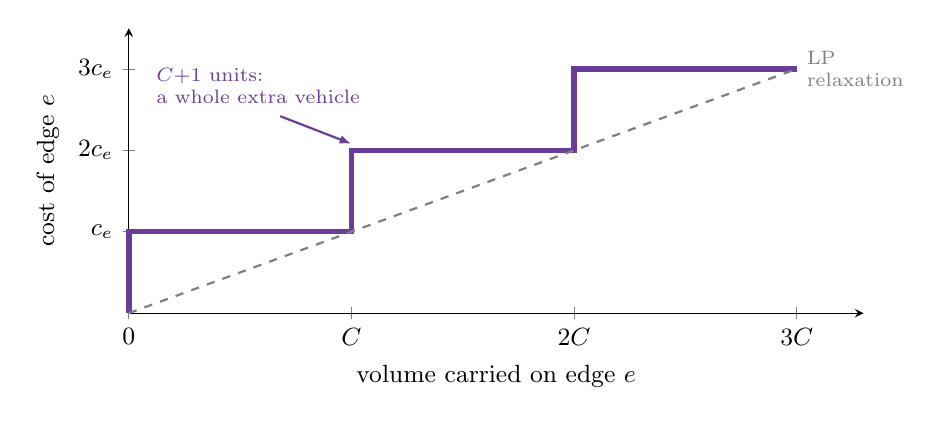
\begin{tikzpicture}
\begin{axis}[width=0.9\linewidth,height=5.2cm,xlabel={volume carried on edge $e$},ylabel={cost of edge $e$},
  xtick={0,50,100,150},xticklabels={0,$C$,$2C$,$3C$},ytick={1,2,3},yticklabels={$c_e$,$2c_e$,$3c_e$},
  ymin=0,ymax=3.5,xmin=0,xmax=165,axis lines=left,clip=false,label style={font=\small},tick label style={font=\small}]
\addplot[const plot mark right,line width=2pt,cStep] coordinates {(0,0)(0.01,1)(50,1)(50.01,2)(100,2)(100.01,3)(150,3)};
\addplot[dashed,gray,thick] coordinates {(0,0)(150,3)} node[pos=1,right,font=\scriptsize,text=gray,align=left] {LP\\relaxation};
\node[font=\scriptsize,text=cStep,align=left,anchor=south west] at (axis cs:4,2.45) {$C{+}1$ units:\\a whole extra vehicle};
\draw[-{Latex[length=1.5mm]},cStep,thick] (axis cs:34,2.42) -- (axis cs:50,2.08);
\end{axis}
\end{tikzpicture}

{\scriptsize schematic, $C=50$}
\column{0.5\textwidth}
\begin{block}{The billed quantity is the vehicle count}
\[
\text{cost of } e = \textcolor{cStep}{c_e\,y_e},\qquad y_e\in\Int_+
\]
with enough vehicles for the flow: $\sum_{k} x^k_e \le C\,y_e$
\end{block}
\begin{itemize}
\item a non-convex \emph{staircase} in the volume, shared by all requests on the edge
\item dropping integrality gives the line $c_e x/C$: the LP relaxation, polynomial but \emph{loose}
\end{itemize}
\end{columns}
\note{Practitioners recognise the staircase instantly; OR people recognise a
step-cost network design problem (Gabrel, Knippel, Minoux 1999; Croxton,
Gendron, Magnanti 2003). How loose: the LP solution with vehicles rounded up,
our starting solution, costs $1.19\times$ the GVNS solution at $|V|=10$,
$2.8\times$ at $|V|=50$ and $2.2$--$3.1\times$ at $|V|\ge90$ (Table~2).}
\end{frame}

\begin{frame}{Feature 2: every storage has a reload ceiling}
\begin{columns}[T]
\column{0.46\textwidth}
\centering
\begin{tikzpicture}[scale=0.72]
  \node[storage,minimum size=13mm,fill=cCap!60,font=\normalsize] (h) at (0,0) {$v$};
  \foreach \a/\c in {150/cN1,180/cN2,210/cOK} {\draw[flow,draw=\c] (\a:2.3) -- (h);}
  \foreach \a/\c in {30/cN1,0/cN2,-30/cOK} {\draw[flow,draw=\c] (h) -- (\a:2.3);}
  \draw[flow,draw=gray,dashed] (-2.4,-1.7) -- (-1.0,-1.0);
  \node[lbl,text=gray,align=left,anchor=north] at (-1.3,-1.85) {no room left:\\this request must detour};
  \draw[thick,mDarkTeal] (2.9,-0.9) rectangle (3.3,0.9);
  \fill[cCap!70] (2.9,-0.9) rectangle (3.3,0.9);
  \node[lbl,right] at (3.4,0.9) {$W_v$};
  \node[lbl,right,align=left] at (3.4,0.1) {transit flow\\$=W_v$};
  \node[lbl,right,text=cCap] at (3.4,-0.75) {$\ovl_v=1.0$};
\end{tikzpicture}

\medskip
{\small congestion of a storage in a solution:\\
$\ovl_v = \text{transit flow through } v\,/\,W_v$\\
$1.0$ = at capacity}
\column{0.54\textwidth}
\begin{block}{Transit volume through $v$ is bounded}
\[
\textcolor{cCap}{\sum_{k\in K:\,v\neq s_k,t_k}\ \sum_{e\in\delta^-(v)} x^k_e \;\le\; W_v}
\qquad\forall v\in V
\]
\end{block}
\begin{itemize}
\item once a storage is at capacity, further transit must detour: a longer route or a reload at a less loaded storage
\item origin and destination handling is not transshipment: a direct $s_k\!\to\!t_k$ route touches no node capacity
\end{itemize}
\end{columns}
\note{Node throughput bounds are familiar from hub location (Alumur \& Kara
2008), not from the MCND literature. $\ovl_v$ returns twice: it colours the
Germany map and it drives neighbourhood $N_3$.}
\end{frame}

\begin{frame}{Why not simply run a published network-design code?}   % [optional]
\centering
\footnotesize
\renewcommand{\arraystretch}{1.15}
\begin{tabular}{@{}l>{\raggedright\arraybackslash}p{4.6cm}>{\raggedright\arraybackslash}p{5.4cm}@{}}
\toprule
 & \textbf{fixed-charge capacitated MCND} & \textbf{this problem}\\
\midrule
arc cost & fixed charge per opened arc $+$ linear flow cost & \textcolor{cStep}{$c_e$ per vehicle: a staircase in the volume}\\
capacities & per arc & per arc (through vehicles) \textbf{and} \textcolor{cCap}{per node: transit volume $\le W_v$}\\
extra cost term & --- & reload $f_v$ per unit at every transit node\\
comparable published code & several (tabu, local branching, matheuristics) & none that we know of\\
\bottomrule
\end{tabular}

\medskip
\begin{alertblock}{Consequence for the experimental design}
no published network-design code that we know of charges per vehicle and bounds node throughput, and our open corpus has no published
objective values: we compare GVNS against \textbf{valid bounds} and \textbf{MIP solvers on the same model}
\end{alertblock}
\note{Skip in a 20-minute slot and say the consequence on the yardstick
slide. Literature, if asked (also on the backup slide ``Where it sits''):
capacitated MCND -- Gendron, Crainic, Frangioni 1999; Crainic 2000; column
generation / branch-and-price -- Barnhart et al.\ 1998; cycle-based tabu --
Ghamlouche, Crainic, Gendreau 2003; local branching -- Rodr\'iguez-Mart\'in \&
Salazar 2010; MILP-in-the-loop matheuristics -- Hewitt, Nemhauser, Savelsbergh
2010; survey -- Crainic \& Gendreau 2021. Step costs -- Gabrel, Knippel,
Minoux 1999; Croxton, Gendron, Magnanti 2003. Node capacity -- hub location,
Alumur \& Kara 2008. VNS -- Mladenovi\'c \& Hansen 1997; Hansen et al.\ 2017;
Hansen \& Mladenovi\'c 2019; multi-start VNS for single-path MCF -- Masri et
al.\ 2015; GVNS on CVRP -- Amous et al.\ 2017. Our own real-life logistic
heuristics: truck-and-trailer routing with time windows and split deliveries
(Batsyn \& Ponomarenko 2014, 2015).}
\end{frame}

% ---------------------------------------------------------------------------
\section{Model}

\begin{frame}{The model: an arc-based MILP}
\small
$x^k_e\in\Real_+$: flow of request $k$ on edge $e$;\quad
$y_e\in\Int_+$: vehicles on $e$;\quad $|K|\cdot|E|+|E|$ variables.
\vspace{-6pt}
\begin{align*}
\min\;& \textcolor{cStep}{\sum_{e\in E} c_e\,y_e}
 \;+\;\sum_{k\in K}\ \sum_{\substack{v\in V\\ v\neq s_k,t_k}}\ \sum_{e\in\delta^-(v)} f_v\,x^k_e
 &&\text{vehicles $+$ reloads}\\[-2pt]
\text{s.t.}\;&
\sum_{e\in\delta^+(v)} x^k_e-\sum_{e\in\delta^-(v)} x^k_e=
 \begin{cases} d_k & v=s_k\\ -d_k & v=t_k\\ 0 & \text{otherwise}\end{cases}
 && \forall k,\ \forall v \quad\text{(demand)}\\[-2pt]
&\textcolor{cStep}{\sum_{k\in K} x^k_e\le C\,y_e} && \forall e\in E \quad\text{(vehicle capacity)}\\
&\textcolor{cCap}{\sum_{k\in K:\,v\neq s_k,t_k}\ \sum_{e\in\delta^-(v)} x^k_e \le W_v} && \forall v\in V \quad\text{(transshipment capacity)}\\
& x\ge 0,\quad y\in\Int_+^{|E|}
\end{align*}
\vspace{-4pt}
linear objective and constraints, integer $y$, continuous $x$: a MILP, NP-hard.
This arc model is exactly what the exact solvers (HiGHS, SCIP) receive later.
\note{Read the equations once; every term was just seen in pictures. The
path-based twin has $\sum_k|\Pi_k|+|E|$ variables. Spoken bridge to the
method if the next frame is skipped: relaxing $y$ gives a per-unit path price,
travel$/C$ plus one reload per transit node, so the relaxation wants cheap
transit-free paths; that is why the start solution is every request on its
direct edge, and why $N_1$ searches with a reload-aware metric.}
\end{frame}

\begin{frame}{Path form, and what the LP relaxation tells us}   % [optional]
\begin{columns}[T]
\column{0.6\textwidth}
\textbf{Path form.} Flow $x^k_p$ on paths $p\in\Pi_k$ (all $s_k\!\to\!t_k$ paths),
$\sum_{p\in\Pi_k}x^k_p=d_k$, same $y_e$; only the paths that carry flow matter.

\medskip
\textbf{Relax integrality.} The capacity constraint becomes tight, so
$y_e=\frac1C\sum_k\sum_{p\ni e}x^k_p$ and $y$ disappears:
\[
\min\ \sum_{k\in K}\sum_{p\in\Pi_k} x^k_p\;
\underbrace{\Bigg(\frac1C\sum_{e\in p} c_e+\sum_{\substack{v\in p\\ v\neq s_k,t_k}} f_v\Bigg)}_{\text{per-unit price of path } p}
\]
\column{0.4\textwidth}
\centering
\begin{tikzpicture}
  \node[storage] (s) at (0,0) {$s$};
  \node[storage,fill=cCap!30] (v) at (2,0.9) {$v$};
  \node[storage] (t) at (4,0) {$t$};
  \draw[flow] (s) -- node[lbl,above left] {$c_{sv}/C$} (v);
  \draw[flow] (v) -- node[lbl,above right] {$c_{vt}/C$} (t);
  \node[lbl,text=cCap,above=1mm of v] {$+\,f_v$};
  \draw[road,dashed] (s) -- node[lbl,below] {$c_{st}/C$, no reload} (t);
\end{tikzpicture}

\medskip
\begin{block}{Reading}
a unit of flow pays \emph{travel}$/C$ plus one reload per transit node: the relaxation prefers cheap, transit-free paths
\end{block}
\end{columns}
\medskip
\begin{itemize}
\item on the completed graph the relaxed optimum puts every request on its direct edge: our \textbf{starting solution}; the search metric of $N_1$ is an edge-wise version of this price
\end{itemize}
\note{Bridge from model to method; skip in a 20-minute slot (the model frame's
note has the spoken version). $N_1$'s metric $c'_{vu}=f_v+f_u+c_{vu}/C$ is
edge-wise, so a transit reload is charged on both incident edges; it is a
ranking metric for path generation, not the objective---the MILP prices every
path exactly.}
\end{frame}

% ---------------------------------------------------------------------------
\section{The GVNS}

\begin{frame}{GVNS at a glance}
\centering
\begin{tikzpicture}[node distance=5mm and 6mm, box/.append style={text width=2.75cm,font=\scriptsize}]
  \node[box] (init) {\textbf{initial solution}\\rounded LP:\\every request on its direct edge};
  \node[box,right=of init,fill=cN2!15] (shake) {\textbf{Shake} in $N_k$\\diversified\\random paths\\MILP budget $\tau_{\mathrm{shk}}$};
  \node[box,right=11mm of shake,fill=cN1!15] (vnd) {\textbf{VND} $N_1\!\to\!N_2\!\to\!N_3$\\restart at $N_1$ on improvement\\MILP budget $\tau_{\mathrm{vnd}}$};
  \node[box,right=of vnd,text width=1.6cm] (test) {$z<z_0$?};
  \draw[road] (init) -- (shake);
  \draw[road] (shake) -- node[lbl,above=2pt,font=\scriptsize] {$z_0\gets z$} (vnd);
  \draw[road] (vnd) -- (test);
  \draw[road,draw=cOK] (test.south) -- ++(0,-0.55) -| node[pos=0.25,below,font=\scriptsize,text=cOK] {yes: $k\gets1$} (shake.south);
  \draw[road,draw=cN3] (test.south) -- ++(0,-1.15) -| node[pos=0.25,below,font=\scriptsize,text=cN3] {no: $k\gets k+1$} ($(shake.south)+(-0.5,0)$);
\end{tikzpicture}

\medskip
\begin{itemize}
\item \textbf{search space: commodity paths.} A solution is a path pool $P$ with flows $x$; vehicle counts follow, $y_e=\big\lceil\frac1C\sum_k x^k_e\big\rceil$
\item \textbf{shake and VND are the same primitive} (next slide): the shake adds more, random paths with a larger MILP budget
\item \textbf{stop} when $k>3$ or after $t_{\max}=2|V|$ minutes; a move is accepted \emph{only if it improves}, so the shake never degrades the incumbent, and $k$ advances when the VND fails to beat the post-shake value $z_0$
\end{itemize}
\note{Preprocessing: complete the graph, build the reload-aware graph $G'$,
precompute 20 shortest paths per request. Shake vs VND path counts: 5 random
pool paths vs 1--3 for $N_1$; stop at 3 fully loaded paths / $5C$ free room vs 2 / $1C$ for $N_2$;
3 detours vs 1 for $N_3$. Budgets: $\tau_{\mathrm{shk}}=10+|V|$ / $100+2|V|$\,s,
$\tau_{\mathrm{vnd}}=25$ / $70$\,s ($N_1$ / rest; 15 / 50\,s at $|V|=100$), so
for $N_1$ the shake budget is smaller than the VND budget while $|V|\le14$.
A VNS-school listener will ask whether this is a shake: it is Algorithm~1
called with diversified generation and $\tau_{\mathrm{shk}}$; diversification
comes from the random paths pushed into the pool and the MILP re-optimisation,
and a non-improving shake is discarded. All parameters are on the backup slide
``Settings''.}
\end{frame}

\begin{frame}{Preprocessing and the starting solution}   % [optional]
\begin{columns}[T]
\column{0.5\textwidth}
\centering
\begin{tikzpicture}[scale=0.68]
  \node[storage] (a) at (0,0) {$a$};
  \node[storage] (b) at (1.6,1.2) {$b$};
  \node[storage] (c) at (3.2,0.2) {$c$};
  \node[storage] (d) at (1.8,-1.2) {$d$};
  \draw[road] (a) -- (b); \draw[road] (b) -- (c); \draw[road] (a) -- (d); \draw[road] (d) -- (c);
  \node[lbl,text=black] at (1.6,-2.0) {(a) raw road graph};
  \begin{scope}[xshift=6.0cm]
  \node[storage] (a2) at (0,0) {$a$};
  \node[storage] (b2) at (1.6,1.2) {$b$};
  \node[storage] (c2) at (3.2,0.2) {$c$};
  \node[storage] (d2) at (1.8,-1.2) {$d$};
  \draw[road] (a2) -- (b2); \draw[road] (b2) -- (c2); \draw[road] (a2) -- (d2); \draw[road] (d2) -- (c2);
  \draw[road,dashed,draw=cN1] (a2) -- node[lbl,text=cN1,above,pos=0.78] {$c_{ac}$} (c2);
  \draw[road,dashed,draw=cN1] (b2) -- (d2);
  \node[lbl,text=black] at (1.6,-2.0) {(b) completed graph};
  \end{scope}
\end{tikzpicture}
\column{0.5\textwidth}
\begin{itemize}
\item road graphs are sparse ($a\!\to\!c$ needs a stop); on the raw graph a missing origin--destination path can even make an instance infeasible
\item \textbf{completion}: join every ordered pair by an edge costing the shortest path in $G$ ($c_{ac}$): the cheapest \emph{stop-free} route, touching no $W_v$
\item the exact solvers get the same completed graph ($|E|=|V|(|V|-1)$)
\end{itemize}
\end{columns}
\smallskip
\begin{block}{Start: the rounded LP}
every request on its direct edge (the relaxed optimum), vehicles rounded up: always feasible, and poor ($1.19\times$ GVNS at $|V|=10$, $2.80\times$ at 50, $3.14\times$ on European Russia)
\end{block}
\note{Skip in a 20-minute slot: say ``we complete the graph so every request
has a direct stop-free edge, and start from the rounded LP''. On the raw graph
the node capacities also shrink the feasible region (paper, Sec.~3.2). Many of the
trucks on those direct edges leave partly empty---that is what $N_2$ will fix.
The initial MILP that sets up the flows has a 300\,s limit.}
\end{frame}

\begin{frame}{The move primitive: propose paths, let the MILP redistribute}
\centering
\begin{tikzpicture}[node distance=5mm]
  \node[box,fill=cN1!10] (gen) {\textbf{GenPaths}$(N,k)$\\new candidate paths $Q$\\for every request $k$};
  \node[box,right=of gen] (milp) {\textbf{MILP} on pool $P\cup Q$\\redistribute flow: warm start $x$,\\time limit $\tau$, gap 1\%};
  \node[box,right=of milp,fill=cOK!10] (keep) {improved ($z'<z$)?\\keep new paths with $x'_p>0$,\\prune every zero-flow path};
  \node[box,below=3mm of keep,fill=cCap!10,text width=3.6cm] (drop) {not improved: discard $Q$};
  \draw[road] (gen) -- (milp);
  \draw[road] (milp) -- (keep);
  \draw[road] (milp.east) -- ++(0.35,0) |- (drop.west);
\end{tikzpicture}

\medskip
\begin{columns}[T]
\column{0.5\textwidth}
\begin{block}{Why paths and not edge flows}
per-edge flows are strongly coupled across requests, so a feasible change needs the whole network at once; a path describes one request only, and \emph{adding} a path to a feasible solution never makes it worse
\end{block}
\column{0.5\textwidth}
\begin{itemize}
\item the three neighbourhoods differ \emph{only} in \textbf{GenPaths}; everything else is shared
\item pruning zero-flow paths keeps the in-loop MILP small enough for budgets of 25--70\,s (VND) and $10{+}|V|$ to $100{+}2|V|$\,s (shake)
\item the neighbourhood proposes, the MILP disposes
\end{itemize}
\end{columns}
\note{This is the matheuristic core; OR people will map it to MILP-in-the-loop
schemes (Hewitt et al.). The MILP is HiGHS with a 1\% gap target.}
\end{frame}

\begin{frame}{\textcolor{cN1}{$N_1$}: reload-aware shortest paths}
\begin{columns}[T]
\column{0.45\textwidth}
\centering
\begin{tikzpicture}[scale=1.15]
  \node[storage] (s) at (0,0) {$s$};
  \node[storage,fill=cCap!30] (h) at (2.2,1.1) {$h$};
  \node[storage] (t) at (4.4,0) {$t$};
  \draw[road,draw=cN1,line width=1.5pt] (s) -- node[lbl,above left,text=cN1] {$c'_{sh}$} (h);
  \draw[road,draw=cN1,line width=1.5pt] (h) -- node[lbl,above right,text=cN1] {$c'_{ht}$} (t);
  \draw[road,draw=cN1,line width=1.5pt] (s) -- node[lbl,below,text=cN1] {$c'_{st}$} (t);
  \foreach \i in {1,...,6} {\draw[cN1!30,line width=0.6pt] (0.2,-0.9-0.13*\i) -- (3.0,-0.9-0.13*\i);}
  \foreach \i in {1,2,3} {\draw[cN1,line width=1pt] (0.2,-0.9-0.13*\i) -- (3.0,-0.9-0.13*\i);}
  \node[lbl,right,text=cN1,align=left] at (3.1,-1.35) {pool of 20 paths\\per request};
\end{tikzpicture}
\column{0.55\textwidth}
\begin{block}{Auxiliary complete graph $G'$: per-unit weights}
\[
c'_{vu}=f_v+f_u+\frac{c_{vu}}{C}\qquad\forall (v,u)\in E
\]
travel per unit plus the reloads at the endpoints; plain shortest paths would ignore the reloads
\end{block}
\begin{itemize}
\item 20 shortest paths per request under $c'$, precomputed once; new paths come from this pool
\item \textbf{VND}: $\{1,2,3\}$ new paths per request $\times$ \{random, low-cost first\}; \textbf{Shake}: 5 random pool paths
\item ablation: without $N_1$, $+0.8\%$ (median, synthetic and real alike)
\end{itemize}
\end{columns}
\note{Keep short: $N_2$ is where the money is. If a sharp listener notes that
$c'$ charges a transit reload on both incident edges and also prices origin
and destination reloads: $c'$ is a ranking metric for path generation, not the
objective; the MILP prices every path exactly, so the double count only changes
which 20 paths enter the pool.}
\end{frame}

\begin{frame}{\textcolor{cN2}{$N_2$}: fill the half-empty trucks}
\begin{columns}[T]
\column{0.46\textwidth}
\centering
\begin{tikzpicture}[x=1cm,y=1cm,scale=0.8]
  \node[font=\footnotesize] at (2.7,1.35) {edge $(u,v)$: 110 units, $y_{uv}=\lceil 110/50\rceil=3$};
  \foreach \i/\l in {0/50, 1/50, 2/10} {
    \draw[thick,mDarkTeal] (\i*1.9,0) rectangle ++(1.6,0.7);
    \fill[cN1!60] (\i*1.9,0) rectangle ++(1.6*\l/50,0.7);
    \node[font=\scriptsize] at (\i*1.9+0.8,-0.3) {\l\,/\,50};
  }
  \draw[{Latex}-{Latex},cN2,line width=1.5pt] (3.8+0.33,0.35) -- (3.8+1.58,0.35);
  \node[font=\scriptsize,text=cN2,align=center] at (4.75,0.95) {40 units free};
  \node[font=\footnotesize,align=center] at (2.7,-1.15) {$\load_{uv}=110 \bmod 50 = 10$:\\up to 40 more units here cost \textbf{no extra vehicle}\\and may free one elsewhere};
\end{tikzpicture}

\medskip
\begin{itemize}
\item shortest paths on $G''$ run through partially loaded vehicles
\item dynamic number of new paths per request: stop after 2 fully loaded paths or accumulated free room $\ge1C$ (VND); 3 fully loaded paths or $\ge5C$ (Shake)
\end{itemize}
\column{0.54\textwidth}
\begin{block}{Graph $G''$ favours free room ($\alpha=0.5$)}
\small
\begin{gather*}
c''_{vu}=f_v+f_u+\frac{\load_{vu}}{C}\Big(\frac{c_{vu}}{C}\Big)^{\!\alpha}\\[-2pt]
\load_e=\Big(\textstyle\sum_k\sum_{p\ni e}x^k_p\Big)\bmod C
\end{gather*}
fully loaded edges ($\load_e=0$) keep their $G'$ weight; smaller residual load $\Rightarrow$ lower weight
\end{block}
\begin{alertblock}{Ablation: the dominant operator}
without $N_2$: $+3.9\%$ synthetic, $+1.6\%$ real (medians), up to $+23.8\%$ on a single instance
\end{alertblock}
\end{columns}
\note{Slow down here. Vehicle consolidation is the main lever on the
objective. On the synthetic ablation subset the mean loss is $+7.1\%$ and the
worst case $+23.8\%$ (50\_nodes\_2); on the real subset the mean is $+2.6\%$
and Germany loses $7.6\%$ (components\_A.csv); none of these is corpus-wide.}
\end{frame}

\begin{frame}{\textcolor{cN3}{$N_3$}: detour around the saturated storage}
\begin{columns}[T]
\column{0.48\textwidth}
\centering
\begin{tikzpicture}
  \node[storage] (a) at (0,0) {$s$};
  \node[storage,minimum size=10mm,fill=cCap!70] (b) at (2.4,0) {$v^\ast$};
  \node[storage] (c) at (4.8,0) {$t$};
  \node[storage,fill=cN1!20] (d) at (2.4,-1.6) {$w$};
  \draw[road] (a) -- (b); \draw[road] (b) -- (c);
  \draw[cCap,line width=1.5pt] (b.north west) -- (b.south east); \draw[cCap,line width=1.5pt] (b.north east) -- (b.south west);
  \draw[flow] (a) to[bend right=25] (d); \draw[flow] (d) to[bend right=25] (c);
  \node[lbl,text=cCap,above=1.5mm of b] {$\ovl_{v^\ast}\approx1$: removed from $G'$};
  \node[lbl,below=1mm of d] {new shortest path through a less loaded $w$};
\end{tikzpicture}

\medskip
{\small in the current solution:\\[2pt]
$\ovl_v=\dfrac1{W_v}\displaystyle\sum_{k:\,v\neq s_k,t_k}\ \sum_{p\in\Pi_k:\,v\in p}x^k_p$}
\column{0.52\textwidth}
\begin{itemize}
\item delete the \textbf{single most congested} storage from $G'$ (unless it is the request's own origin or destination), recompute the shortest path: a detour to less loaded storages
\item 1 new path per request in VND, 3 in Shake
\item ablation: $+0.1\%$ / $+0.2\%$ median, \textbf{inactive when capacities are slack}; $+4.0\%$ on Germany, where almost every storage runs at capacity
\end{itemize}
\end{columns}
\note{Say ``situational'' out loud: the operator is worth carrying only for
tight instances---when capacities are slack there is nothing to route around.
Point back at the Germany map. If asked why a single node: removing a prefix
of $|V|/5$--$|V|/4$ congested storages was tried on all 50 instances $\times$
10 seeds; it is indistinguishable on 44 of 50 (within across-seed noise) yet
forfeits $N_3$'s benefit on the capacity-tight networks, so the surgical
version is kept---state the measured outcome, not a mechanism.}
\end{frame}

% ---------------------------------------------------------------------------
\section{Experiments}

\begin{frame}{The benchmark: realistic regional networks, openly available}
\begin{columns}[T]
\column{0.56\textwidth}
\begin{itemize}
\item our open corpus (arXiv:2606.20653; Zenodo, CC-BY-4.0), every instance reproducible from its published seed
\item road networks between regional sorting centres, calibrated on OpenStreetMap for \textbf{nine European countries, five U.S.\ states and European Russia}
\item real structure: Zipf city sizes, spatial-network topology, centrality-driven $W_v$, gravity demand; near-planar, large-diameter graphs
\item \textbf{35 synthetic}: $10\times|V|{=}10$, $7\times20$, $7\times30$, $5\times50$, $3\times100$, $3\times150$
\item \textbf{15 real-geometry}: Denmark ($|V|=11$) to European Russia ($|V|=90$)
\end{itemize}
\column{0.44\textwidth}
\centering
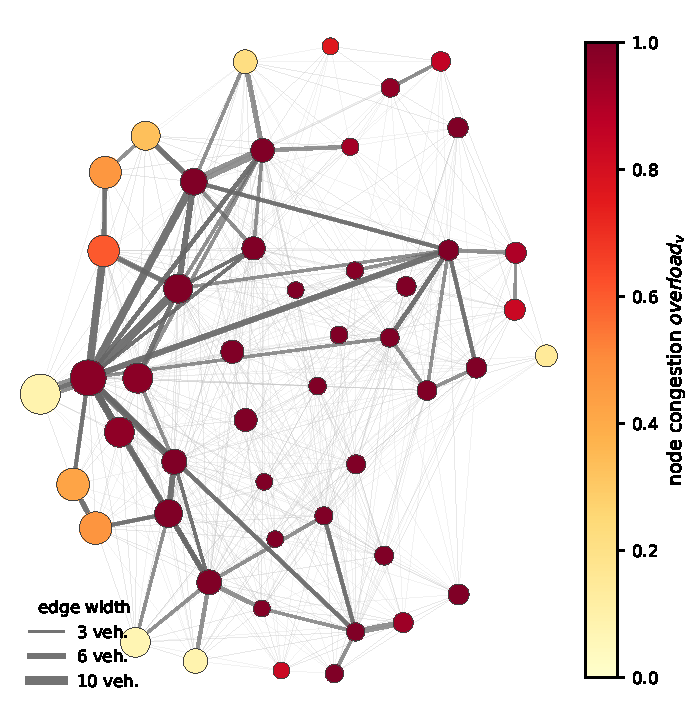
\includegraphics[height=0.52\textheight]{figs/germany_solution.pdf}

{\scriptsize Germany ($|V|=49$), the solution from the first slide:
almost every storage runs at capacity.\par}
\end{columns}
\note{The generator is a separate paper; here only what the study needs.
Mean degree is 3.575 in the paper. Point at the map: thick edges are
consolidation ($N_2$) made visible, dark nodes are what $N_3$ works on. The
instance's numbers come where they are defined: $\gapLB=11.0\%$, exact
incumbent $1.544\times$, rounded-LP start $2.692\times$, $\sigma$ over 10 seeds
$2.0\%$; without $N_2$ $+7.6\%$, without $N_3$ $+4.0\%$.}
\end{frame}

\begin{frame}{Setup and yardsticks}
\centering
\begin{tikzpicture}[x=1cm]
  \draw[-{Latex[length=2.5mm]},thick,mDarkTeal] (0,0) -- (13.2,0) node[right,font=\scriptsize] {objective};
  \foreach \x/\lab/\val/\col in {0.9/{LP relaxation}/{0.971}/gray, 3.6/{MIP dual bound $\underline{z}$}/{}/cN1, 6.2/{optimum $z^\ast$}/{(unknown)}/gray, 8.8/{GVNS}/{1.0}/mLightBrown, 11.8/{rounded LP (start)}/{1.192}/gray}{
    \draw[thick,\col] (\x,-0.15) -- (\x,0.15);
    \node[font=\scriptsize,text=\col,align=center,above=1mm] at (\x,0.15) {\lab\\ \val};
  }
  \node[font=\scriptsize,text=cOK,align=center,below=1mm] at (8.8,-0.15) {MIP incumbent 1.000};
  \draw[{Bar}-{Bar},thick,cN1] (3.6,-0.75) -- (8.8,-0.75) node[midway,below,font=\scriptsize,text=cN1] {$\gapLB=0.96\%$};
  \node[font=\scriptsize,text=gray] at (11.8,-0.8) {ratios: means at $|V|=10$; not to scale};
\end{tikzpicture}

\smallskip
\begin{columns}[T]
\column{0.48\textwidth}
\begin{block}{Two metrics}
\small
$\gapLB=\big(\mathit{Result}_{\mathrm{GVNS}}-\underline{z}\big)/\underline{z}$,\quad $\underline{z}=$ best MIP dual bound:
an \textbf{upper bound on the true optimality gap} of GVNS\\[3pt]
$\mathit{Ratio}_{\mathrm{method}}=\mathit{Result}_{\mathrm{method}}/\mathit{Result}_{\mathrm{GVNS}}$:
below 1 better than GVNS, above 1 worse
\end{block}
\column{0.52\textwidth}
\begin{itemize}\small
\item GVNS: 10 seeds per instance, limit $2|V|$\,min; exact: gap target 0, 30\,min--4\,h, i.e.\ comparable budgets ($|V|=50$: 100\,min vs 2\,h); HiGHS is the exact baseline \emph{and} the in-loop solver
\item nothing is proven optimal, but $\underline{z}$ is a valid lower bound, typically within a few percent of the incumbent: $\gapLB$ is a guarantee, not a self-comparison
\end{itemize}
\end{columns}
\note{Hardware: HSE cluster cHARISMa, nodes with 2$\times$AMD EPYC (44 cores,
$\ge$720\,GB RAM), each job pinned to 8 cores; HiGHS 1.14.0, SCIP 10.0.2 as
cross-check. Exact side in one breath: none of the 50 instances was solved to
proven optimality; up to $|V|=42$ the two solvers' dual bounds agree within
$0.6\%$; SCIP returns nothing usable from $|V|=45$; the arc model is out of
memory at $|V|\ge100$ (backup ``The exact side''). If you accept one number
from this talk, make it $\gapLB$: it bounds the distance to the optimum instead
of comparing GVNS with itself. The ladder ticks are the $|V|=10$ means of
Table~2; the dual bound sits between the LP and GVNS, and GVNS is $0.96\%$
above it.}
\end{frame}

\begin{frame}{Results I: synthetic instances}
\begin{columns}[T]
\column{0.56\textwidth}
\centering
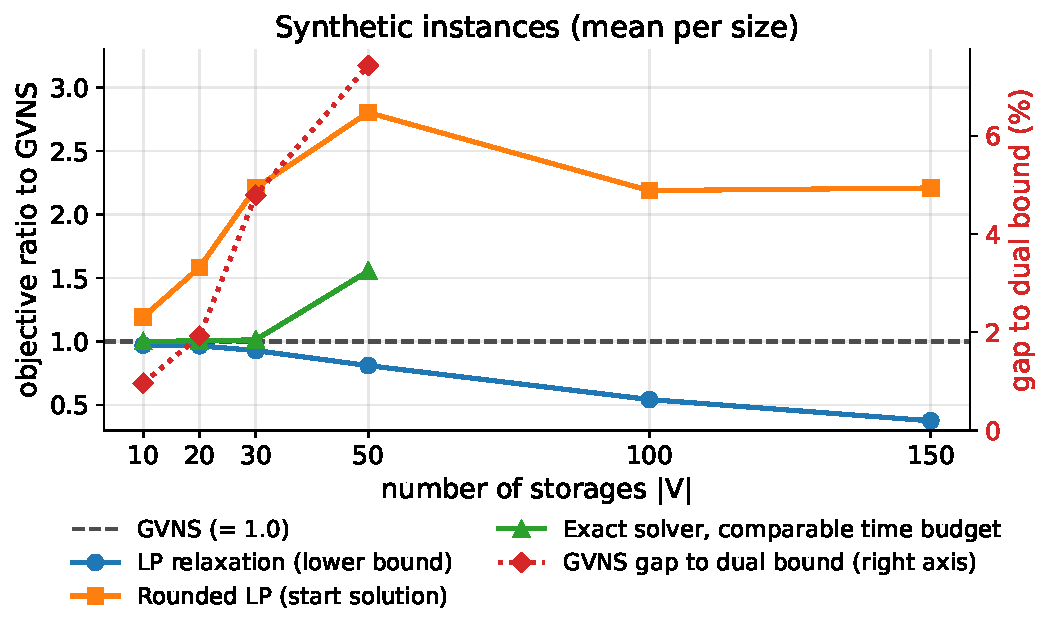
\includegraphics[width=0.94\linewidth]{figs/ratios_synthetic.pdf}
\column{0.44\textwidth}
\centering
\small
\setlength{\tabcolsep}{4pt}
\begin{tabular}{@{}rrccc@{}}
\toprule
$|V|$ & $n$ & $\gapLB$ & exact inc. & $\sigma$\\
\midrule
10  & 10 & 0.96\% & 1.000 & 0.06\%\\
20  & 7  & 1.92\% & 1.005 & 0.18\%\\
30  & 7  & 4.79\% & 1.013 & 0.68\%\\
50  & 5  & 7.44\% & \alert{1.555} & 0.66\%\\
100 & 3  & \dag & \dag & 0.31\%\\
150 & 3  & \dag & \dag & 0.38\%\\
\bottomrule
\end{tabular}

{\scriptsize\dag: arc model intractable; only the loose LP bound (0.542, 0.375)\par}

\smallskip
{\small near-optimal up to $|V|=20$; at $|V|=50$ the exact solver with a comparable budget is \alert{55\% more expensive} on average (16\% to 137\% per instance)\par}
\end{columns}
{\scriptsize GVNS mostly stops before its limit (3\,729 of 6\,000\,s at $|V|=50$); the exact solver always used its full budget, so the comparison is conservative.\par}
\note{Trace the green curve: flat at 1.0, up to 1.555 at 50, then it stops
existing. Spoken: $\gapLB$ is about 1--2\% up to $|V|\approx20$, 4.8\% at 30,
7.4\% at 50, where the LP bound alone would say about 24\%; at $|V|\ge100$
GVNS still ends $2.2\times$ below its own start. Mean run time vs limit:
633/1\,200\,s (10), 1\,952/2\,400 (20), 2\,611/3\,600 (30), 3\,729/6\,000 (50),
5\,983/12\,000 (100), 18\,236/18\,000 (150); the 150-node mean slightly exceeds
its limit because Algorithm~2 tests $t_{\max}$ only before each shake and after
each full VND sweep, so a shake started just under the limit (MILP budget up to
$100+2|V|=400$\,s at $|V|=150$) and the sweep after it run to completion.
Per-instance $|V|=50$ numbers are on the backup slide ``What the means hide''.}
\end{frame}

\begin{frame}{Results II: real road geometries mirror the synthetic story}
\begin{columns}[T]
\column{0.58\textwidth}
\centering
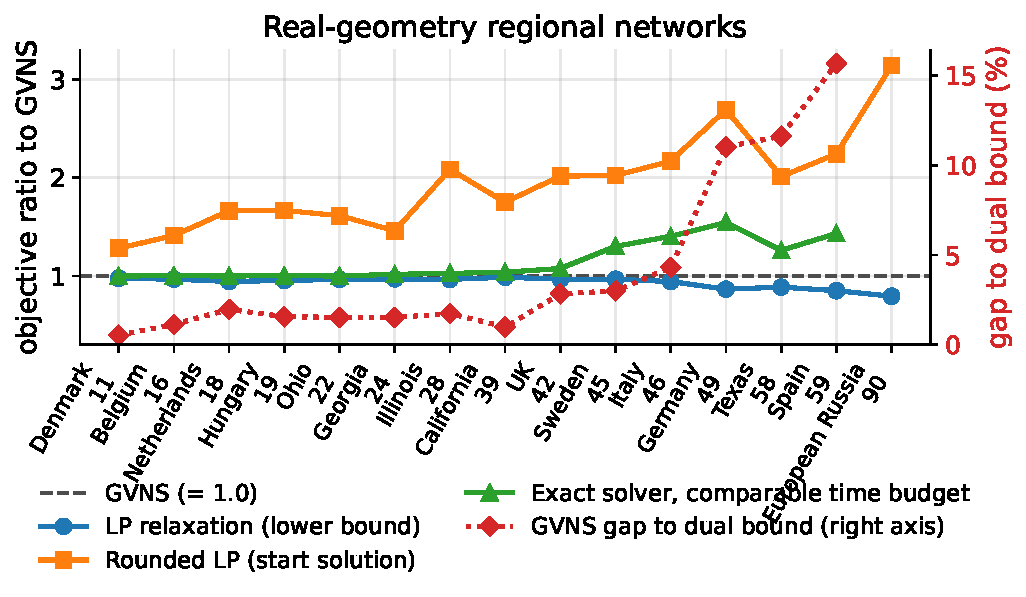
\includegraphics[width=\linewidth]{figs/ratios_real.pdf}
\column{0.42\textwidth}
\begin{itemize}
\item exact solver with a comparable budget: parity up to $|V|=22$, $1.02$--$1.08\times$ up to the UK (42), then \alert{$1.26$--$1.54\times$} from Sweden (45) to Spain (59)
\item $\gapLB$ from $0.5\%$ (Denmark, 11) to $15.7\%$ (Spain, 59)
\item European Russia ($|V|=90$): no exact reference; GVNS ends $3.1\times$ below its start
\end{itemize}
\medskip
{\small\itshape same shape as the synthetic curves: the synthetic corpus behaves like the real geometries, and GVNS is robust to them}
\end{columns}
\note{Do not read the table; point at the three medium networks and at the
90-node one. Spoken detail: $\gapLB$ about 1--3\% up to $|V|=45$, 4.3\% on
Italy (46), 11.0\% Germany (49), 11.6\% Texas (58), 15.7\% Spain (59); exact
incumbent 1.02--1.04$\times$ from Georgia (24) to California (39), 1.077 UK;
run time 615\,s (Denmark) to 3\,986\,s (Spain), 5\,595\,s on European Russia.
Full Table~2 rows are in the paper.}
\end{frame}

\begin{frame}{How many seeds do you need?}   % [optional]
\begin{columns}[T]
\column{0.58\textwidth}
\centering
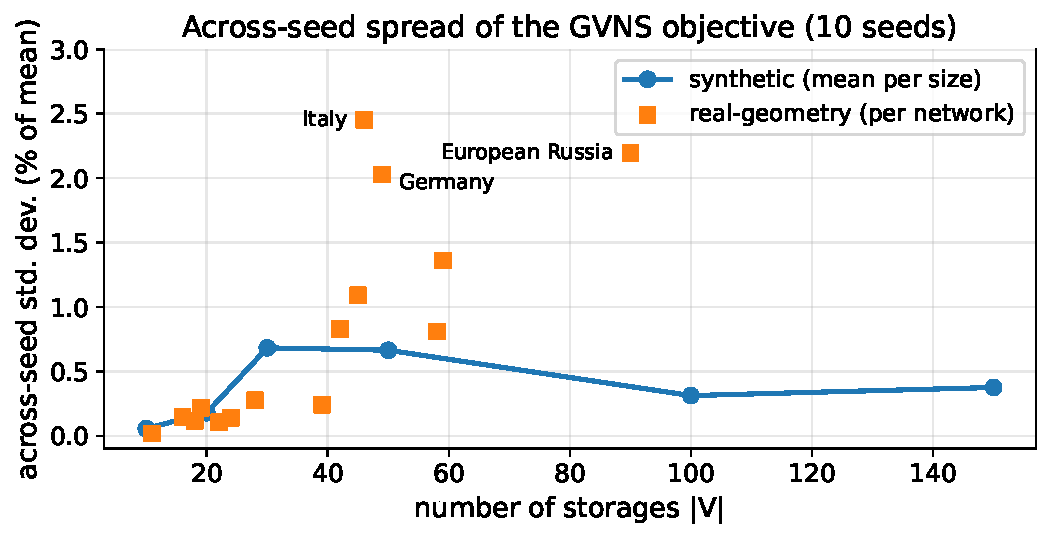
\includegraphics[width=\linewidth]{figs/seed_spread.pdf}
\column{0.42\textwidth}
\begin{itemize}
\item synthetic: across-seed $\sigma$ below $0.7\%$ of the mean at every size, below $0.2\%$ up to $|V|=20$
\item large real networks: $2.0\%$ (Germany), $2.5\%$ (Italy), $2.2\%$ (European Russia)
\item \alert{three seeds badly understate it}: on Italy the spread over three seeds is $0.4\%$ against $2.5\%$ over ten
\item one run is representative on small networks; on capacity-tight instances take the best of several
\end{itemize}
\end{columns}
\note{Backup for the ``is it stable?'' question. We moved from 3 to 10 seeds
for the headline numbers and 5 for the component study.}
\end{frame}

\begin{frame}{What each component buys}
\begin{columns}[T]
\column{0.54\textwidth}
\centering
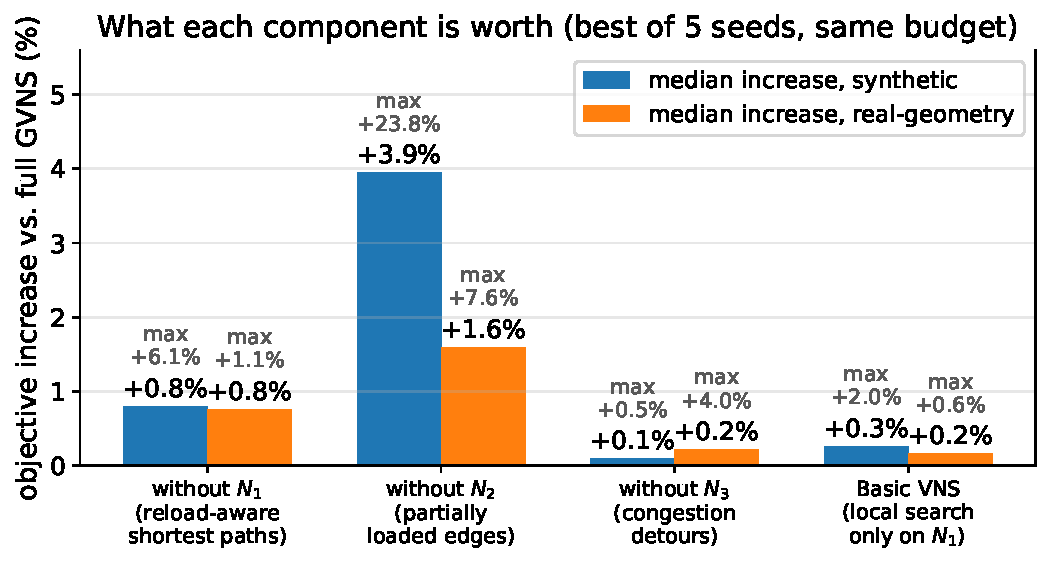
\includegraphics[width=\linewidth]{figs/ablation.pdf}

{\scriptsize best of 5 seeds, same budget, subset of synthetic ($|V|=20$--$100$) and real ($16$--$49$) instances; medians because the seed spread is heavy-tailed on capacity-tight networks\par}
\column{0.46\textwidth}
\footnotesize
\setlength{\tabcolsep}{3pt}
\begin{tabular}{@{}lcc@{}}
\toprule
GVNS better / tie / variant better & synth. & real\\
\midrule
without $N_1$ & 8 / 0 / 1 & 5 / 1 / 0\\
without $N_2$ & 8 / 1 / 0 & 5 / 1 / 0\\
without $N_3$ & 1 / 8 / 0 & 3 / 3 / 0\\
Basic VNS & 5 / 4 / 1 & 2 / 4 / 0\\
\bottomrule
\end{tabular}

{\scriptsize ``decided'' = difference beyond the seed spread of both runs; time relative to GVNS: 0.80, 0.52, 0.68, 0.63\par}

\medskip
\begin{itemize}\small
\item \textcolor{cN2}{$N_2$ dominates}; \textcolor{cN3}{$N_3$ is situational}: ties when capacities are slack, $+4.0\%$ on Germany
\item \textbf{Basic VNS} (local search on $N_1$ only, same shake): GVNS better on 7 of 16, Basic VNS on 1, 8 ties; the margin grows with size, $0.2$--$0.6\%$ at $|V|\le28$ vs $1.1$--$2.0\%$ at $|V|\ge50$, for $1/0.63$ of the time
\end{itemize}
\end{columns}
\note{One line: $N_2$ dominates, the VND matters at scale, $N_3$ is for tight
instances. Table~3's time ratios are the means of the synthetic and real
groups (CSV: $N_1$ 0.76/0.84, $N_2$ 0.54/0.50, $N_3$ 0.73/0.63, Basic VNS
0.68/0.58). The CSV's \texttt{argmax\_instance} names the instance where the
variant is \emph{worst}, not best. Single instances can flip sign: the two
``variant better'' entries in the table are decided (beyond the seed spread of
both runs): 50\_nodes\_2, where dropping $N_1$ improved the result by 2.1\%, and
30\_nodes\_2, where Basic VNS beat GVNS by 1.3\%; Basic VNS also improves
Germany by 4.0\%, but inside its 4.2\% seed spread there, so a tie.}
\end{frame}

% ---------------------------------------------------------------------------
\section{Closing}

\begin{frame}{Limitations, and what comes next}
\begin{columns}[T]
\column{0.5\textwidth}
\textbf{Stated before you ask}
\begin{itemize}\small
\item \textbf{static capacities and costs}: on real networks they vary with the time of day
\item \textbf{no proven optima}: $\gapLB$ is an upper bound on the true gap
\item \textbf{no tight reference beyond $|V|=59$}: only the loose LP bound
\item \textbf{path generation is heuristic}: a pool of 20 shortest paths plus three rules
\item \textbf{open-source solvers at default settings} as the exact baseline (tuning checked on 8 instances)
\item \textbf{component study} on a subset with five seeds; \textbf{no operational data} yet
\end{itemize}
\column{0.5\textwidth}
\textbf{Next}
\begin{itemize}\small
\item time-expanded graph with period-dependent $C_e(t)$, $W_v(t)$: the neighbourhoods only need a period-aware edge metric
\item column-generation pricing to feed the path pool
\item validation on operational data
\end{itemize}
\end{columns}
\note{Justifications, spoken: at $|V|=50$--$59$ the 7--16\% gap cannot be split
between heuristic error and bound weakness; beyond $|V|=59$ the LP bound is
0.795 on European Russia and 0.542 / 0.375 at 100 / 150; HiGHS and SCIP with
three presets each moved nothing (backup ``The exact side''). The ``next''
items answer the first, fourth and last limitations.}
\end{frame}

\begin{frame}{Takeaways}
\begin{enumerate}\setlength{\itemsep}{8pt}
\item \textcolor{cStep}{integer trucks} $+$ \textcolor{cCap}{reload ceilings}: compare against \textbf{valid dual bounds}, not fixed-charge codes
\item path-space GVNS: within $\approx1\%$ of the dual bound on small networks; the exact solver is \textbf{up to 55\% more expensive} at $|V|=50$
\item \textcolor{cN2}{$N_2$} is the lever, \textcolor{cN3}{$N_3$} only when capacity binds, the full VND pays at scale
\end{enumerate}
\bigskip
\begin{center}
{\large\itshape Let cheap path generators propose and a time-boxed MILP dispose:\\
$N_2$ always, $N_3$ when capacity binds, the full VND once the network is large.}
\end{center}
\note{End on the italic sentence; it calls back to ``the neighbourhood
proposes, the MILP disposes'' on the primitive slide.}
\end{frame}

\begin{frame}{Thank you}
\begin{columns}[T]
\column{0.58\textwidth}
\textbf{Code, exact-solver harness, scripts that regenerate every table and figure}\\
{\small\href{https://github.com/aponom84/Optimal-Logistic-Net}{\texttt{github.com/aponom84/Optimal-Logistic-Net}}}

\medskip
\textbf{Instance corpus} (CC-BY-4.0)\\
{\small\href{https://doi.org/10.5281/zenodo.20372456}{\texttt{doi.org/10.5281/zenodo.20372456}}}

\medskip
\textbf{Contact}\\
\texttt{aponomarenko@hse.ru} $\cdot$ \texttt{varvara\_kovaleva03@mail.ru}

\bigskip
{\footnotesize Supported by the Basic Research Program at HSE University
(HSE-BR-2025-080) and by the HPC facilities of HSE University (cHARISMa).\par}
\column{0.42\textwidth}
\centering
\begin{tabular}{c@{\hspace{6mm}}c}
\qrcode[height=2.4cm]{https://github.com/aponom84/Optimal-Logistic-Net} &
\qrcode[height=2.4cm]{https://doi.org/10.5281/zenodo.20372456}\\[3pt]
{\small code} & {\small data}
\end{tabular}
\end{columns}
\note{Question map: seeds -- ``How many seeds''; solver behaviour and tuning --
backup ``The exact side''; per-instance spread at $|V|=50$ -- backup ``What
the means hide''; any parameter -- backup ``Settings''; literature -- backup
``Where it sits''; the $N_3$ prefix variant -- the $N_3$ slide's note.}
\end{frame}

% ---------------------------------------------------------------------------
% Backup slides: no progress bar (its denominator is the appendix frame
% count, which appendixnumberbeamer only knows after the first pass).
\appendix
\metroset{progressbar=none}

\begin{frame}{Backup: settings (Table~1 of the paper)}
\centering
\small
\renewcommand{\arraystretch}{1.15}
\setlength{\tabcolsep}{4pt}
\begin{tabular}{llll}
\toprule
Setting & Value & Setting & Value\\
\midrule
neighbourhoods $k_{\max}$ & 3 & $N_2$ exponent $\alpha$ & 0.5\\
GVNS limit $t_{\max}$ & $2|V|$\,min & $N_2$ free-room stop & $1C$ / $5C$\\
random seeds & 10 / 5 (components) & $N_3$ storages removed & 1 (most congested)\\
vehicle capacity $C$ & 50 & $N_1$ path pool & 20\\
$N_1$ paths per request & 1--3 / 5 & $N_3$ paths per request & 1 / 3\\
initial MILP limit & 300\,s & exact gap target & 0\\
redistribution MILP gap & 1\% & exact budget & 30\,min--4\,h\\
$\tau_{\mathrm{shk}}$ ($N_1$ / rest) & $10{+}|V|$ / $100{+}2|V|$\,s & $\tau_{\mathrm{vnd}}$ ($N_1$ / rest) & 25 / 70\,s ($15$ / $50$\,s at $|V|=100$)\\
\bottomrule
\end{tabular}

\medskip
{\footnotesize Values given as VND / Shake where they differ. Each job pinned to 8 cores;
HSE cluster cHARISMa (2$\times$AMD EPYC, 44 cores, $\ge$720\,GB RAM per node); HiGHS 1.14.0, SCIP 10.0.2.}
\end{frame}

\begin{frame}{Backup: the exact side, and is the baseline understated?}
\centering
\scriptsize
\renewcommand{\arraystretch}{1.05}
\begin{tabular}{@{}l>{\raggedright\arraybackslash}p{4.2cm}>{\raggedright\arraybackslash}p{4.6cm}>{\raggedright\arraybackslash}p{3.2cm}@{}}
\toprule
 & \textbf{HiGHS 1.14} & \textbf{SCIP 10} & \textbf{arc MILP size}\\
\midrule
$|V|\le 42$ & dual bound $+$ incumbent & dual bound agrees with HiGHS within $0.6\%$ (mean $0.18\%$); weaker incumbent & $\approx6\,000$ variables at $|V|=10$\\
$|V|=45$--$59$ & dual bound $+$ incumbent & \textcolor{cCap}{no feasible solution, no non-trivial bound} & \\
$|V|\ge 90$ & \multicolumn{2}{>{\raggedright\arraybackslash}p{9cm}}{millions of variables: at $|V|=90$ only SCIP was tried and returns no bound and no incumbent; \textcolor{cCap}{out of memory} for both at $|V|\ge100$} & $3.7\times10^{8}$ at $|V|=150$\\
\bottomrule
\end{tabular}

\smallskip
\begin{columns}[T]
\column{0.5\textwidth}
\scriptsize
budgets: MIP-gap target 0, 30\,min ($|V|=10$) to 4\,h ($|V|=150$); \alert{none of the 50 instances solved to proven optimality}, but the branch-and-bound dual bound is tight and well above the LP.

\smallskip
\textbf{Tuning check}: 8 instances ($|V|=30$--$59$), three non-default presets per backend (HiGHS: aggressive heuristics, presolve off, full parallelism; SCIP: aggressive heuristics, feasibility emphasis, aggressive separation). SCIP: no preset helps; two presets \emph{degrade} the dual bound by up to $2.3\%$ and the incumbent by up to $48\%$; on the six subset instances with $|V|\ge45$ no preset finds a feasible solution.

\smallskip
\alert{\textbf{The default configuration does not understate the exact baseline.}}
\column{0.5\textwidth}
\centering
\scriptsize
\setlength{\tabcolsep}{4pt}
\begin{tabular}{@{}lrr@{}}
\toprule
instance & \multicolumn{2}{c}{HiGHS, column-wise best of 3 presets vs default}\\
 & dual bound & incumbent\\
\midrule
30\_nodes\_1 & $+0.005\%$ & $+0.054\%$\\
30\_nodes\_2 & $+0.015\%$ & $0$\\
50\_nodes\_1 & $+0.002\%$ & $+0.285\%$\\
50\_nodes\_2 & $0$ & $0$\\
Sweden (45) & $+0.003\%$ & $+0.823\%$\\
Germany (49) & $+0.023\%$ & $+0.108\%$\\
Texas (58) & $+0.036\%$ & $+0.454\%$\\
Spain (59) & $+0.029\%$ & $+0.885\%$\\
\bottomrule
\end{tabular}

{\scriptsize $+$ = improvement; full grid in \texttt{Results/exact\_tuning.csv}\par}
\end{columns}
\note{HiGHS is the stronger exact solver here and therefore also the in-loop
solver of GVNS. Europe Russia ($|V|=90$) was attempted with SCIP only (time
limit, no bound, no incumbent); the paper reports the arc model as intractable
from about $|V|=90$ and out of memory at $|V|\ge100$.}
\end{frame}

\begin{frame}{Backup: what the means hide at $|V|=50$}
\centering
\small
\setlength{\tabcolsep}{6pt}
\begin{tabular}{@{}lccccr@{}}
\toprule
instance & $\gapLB$ & exact inc. & rounded LP & LP relax. & mean GVNS time\\
\midrule
50\_nodes\_1 & 2.99\% & 1.162 & 2.151 & 0.827 & 2\,890\,s\\
50\_nodes\_2 & \alert{14.61\%} & \alert{2.368} & 4.131 & 0.777 & 5\,583\,s\\
50\_nodes\_3 & 5.25\% & 1.410 & 2.707 & 0.784 & 4\,001\,s\\
50\_nodes\_4 & 9.69\% & 1.523 & 2.668 & 0.854 & 2\,954\,s\\
50\_nodes\_5 & 4.64\% & 1.311 & 2.363 & 0.805 & 3\,215\,s\\
\midrule
mean & 7.44\% & 1.555 & 2.804 & 0.810 & 3\,729\,s\\
\bottomrule
\end{tabular}

\medskip
\begin{itemize}
\item $50\_nodes\_2$ is where the exact solver falls furthest behind of any instance with a dual bound: its incumbent is $2.37\times$ GVNS, the rounded-LP start $4.13\times$; only Spain ($|V|=59$, $15.7\%$) has a larger $\gapLB$
\item on this instance the $14.6\%$ cannot be split between heuristic error and bound weakness; the LP bound alone would put the gap at $29\%$, so the dual bound is already much tighter
\item per-instance $\gapLB$ at the smaller sizes: $0.38$--$1.95\%$ at $|V|=10$, $1.08$--$2.66\%$ at 20, $2.42$--$6.58\%$ at 30
\end{itemize}
\end{frame}

\begin{frame}{Backup: where it sits in the literature}
\begin{columns}[T]
\column{0.5\textwidth}
\textbf{Capacitated multicommodity network design}
\begin{itemize}\scriptsize
\item Gendron, Crainic, Frangioni (1999); Crainic (2000): fixed-charge MCND, NP-hard
\item Barnhart et al.\ (1998): branch-and-price on path formulations
\item Ghamlouche, Crainic, Gendreau (2003): cycle-based tabu search
\item Rodr\'iguez-Mart\'in, Salazar-Gonz\'alez (2010): local branching
\item Hewitt, Nemhauser, Savelsbergh (2010): MILP-in-the-loop matheuristics
\item Crainic, Gendreau (2021): survey of (meta)heuristics
\end{itemize}
\textbf{Step costs and node capacities}
\begin{itemize}\scriptsize
\item Gabrel, Knippel, Minoux (1999): exact Benders-type method for general step costs
\item Croxton, Gendron, Magnanti (2003): MILP models of nonconvex piecewise-linear costs
\item Alumur, Kara (2008): hub location with bounded hub throughput
\end{itemize}
\column{0.5\textwidth}
\textbf{Variable neighbourhood search}
\begin{itemize}\scriptsize
\item Mladenovi\'c, Hansen (1997); Hansen et al.\ (2017); Hansen, Mladenovi\'c (2019): VNS, GVNS
\item Karakostas et al.\ (2019); Mjirda et al.\ (2016): GVNS vs single-neighbourhood schemes
\item Masri, Krichen, Guitouni (2015): multi-start VNS for the single-path multicommodity flow problem
\item Amous et al.\ (2017): VNS for the capacitated VRP
\end{itemize}
\textbf{Real-life logistic routing}
\begin{itemize}\scriptsize
\item Batsyn, Ponomarenko (2014, 2015): truck-and-trailer routing with time windows and split deliveries
\end{itemize}
\textbf{Benchmark}
\begin{itemize}\scriptsize
\item Kovaleva, Ponomarenko (2026): generator and corpus, arXiv:2606.20653, Zenodo 10.5281/zenodo.20372456
\end{itemize}
\end{columns}
\end{frame}

\end{document}
"
% to get the speaker-notes version (see build.sh)
\ifdefined\shownotes
  \setbeameroption{show notes on second screen=right}
\fi

% Colour system carried through the talk:
%   cStep -- feature 1, per-vehicle step cost      cCap -- feature 2, reload ceiling
%   cN1 / cN2 / cN3 -- the three neighbourhoods    (cN3 = cCap: N3 acts on congestion)
\definecolor{cStep}{HTML}{6A3D9A}
\definecolor{cCap}{HTML}{B2182B}
\definecolor{cN1}{HTML}{1F77B4}
\definecolor{cN2}{HTML}{E8710A}
\definecolor{cN3}{HTML}{B2182B}
\definecolor{cOK}{HTML}{2E7D32}

\tikzset{
  storage/.style={circle,draw=mDarkTeal,thick,fill=mDarkTeal!10,minimum size=7mm,inner sep=0pt,font=\small},
  road/.style={-{Latex[length=2mm]},draw=mDarkTeal!60,thick},
  flow/.style={-{Latex[length=2.5mm]},draw=mLightBrown,line width=2pt},
  box/.style={draw=mDarkTeal,thick,rounded corners=2pt,fill=mDarkTeal!5,align=center,font=\small,inner sep=5pt,minimum height=9mm},
  lbl/.style={font=\scriptsize,text=mDarkTeal!80},
  truck/.pic={\draw[fill=white,thick] (-0.28,0) rectangle (0.18,0.22);
              \draw[fill=white,thick] (0.18,0) rectangle (0.32,0.15);
              \fill (-0.18,0) circle(0.045); \fill (0.2,0) circle(0.045);},
}

\newcommand{\Real}{\mathbb{R}}
\newcommand{\Int}{\mathbb{Z}}
\newcommand{\gapLB}{gap_{\mathrm{LB}}}
\newcommand{\ovl}{\mathit{overload}}
\newcommand{\load}{\mathit{load}}
\setlength{\leftmargini}{1.2em}
\setbeamersize{text margin left=0.7cm,text margin right=0.7cm}

\title{A General Variable Neighborhood Search for Logistic Network Flow Design
  with Nonlinear Edge Costs and Transshipment Capacities}
\subtitle{OPTIMA 2026}
\author{Varvara Kovaleva\inst{1} \and Alexander Ponomarenko\inst{2}}
\institute{\inst{1} HSE University, Nizhny Novgorod \and
  \inst{2} Laboratory of Algorithms and Technologies for Network Analysis, HSE University, Nizhny Novgorod}
\date{}

\begin{document}

\maketitle
\note{One breath, then the hook: ``Every night, freight between regional sorting
centres moves in trucks that are either full or not, and every centre can only
reload so much. Those two facts alone break the textbook flow model---this talk
is about what to do instead.''}

% ---------------------------------------------------------------------------
\section{The problem}

\begin{frame}{Freight between regional sorting centres}
\begin{columns}[T]
\column{0.56\textwidth}
\centering
\begin{tikzpicture}[scale=0.82]
  \node[storage,minimum size=8mm] (s) at (0,0) {$s_k$};
  \node[storage,minimum size=11mm,fill=cCap!35] (u) at (2.6,1.5) {$u$};
  \node[storage,minimum size=6mm] (w) at (2.6,-1.2) {$w$};
  \node[storage,minimum size=9mm] (t) at (5.2,0) {$t_k$};
  \draw[road] (s) -- node[lbl,below right,pos=0.55] {$c_{su}$} (u);
  \draw[road] (u) -- node[lbl,below left,pos=0.45] {$c_{ut}$} (t);
  \draw[road] (s) -- node[lbl,below left] {$c_{sw}$} (w);
  \draw[road] (w) -- node[lbl,below right] {$c_{wt}$} (t);
  \draw[road] (s) -- node[lbl,below,pos=0.6] {$c_{st}$ (direct)} (t);
  \draw[flow,opacity=0.85] (s) to[bend left=18] (u);
  \draw[flow,opacity=0.85] (u) to[bend left=18] (t);
  \pic at (1.0,1.15) {truck};
  \node[lbl,text=mLightBrown] at (0.75,1.65) {$C$ units};
  \node[lbl,text=cCap,above=1mm of u,align=center] {reload $f_u$ per unit; at most $W_u$ in transit};
  \node[lbl,left=1mm of s] {demand $d_k$};
\end{tikzpicture}

\medskip
\begin{itemize}\setlength{\itemsep}{2pt}
\item \textbf{storages} $v$: reload cost $f_v$ per unit, \textcolor{cCap}{transshipment capacity $W_v$}
\item \textbf{roads} $e$: cost $c_e$ \textcolor{cStep}{per vehicle}; a vehicle carries $C$ units ($C=50$)
\item \textbf{requests} $k$: ship $d_k$ units from $s_k$ to $t_k$, reloading on the way if useful
\end{itemize}
\column{0.44\textwidth}
\centering
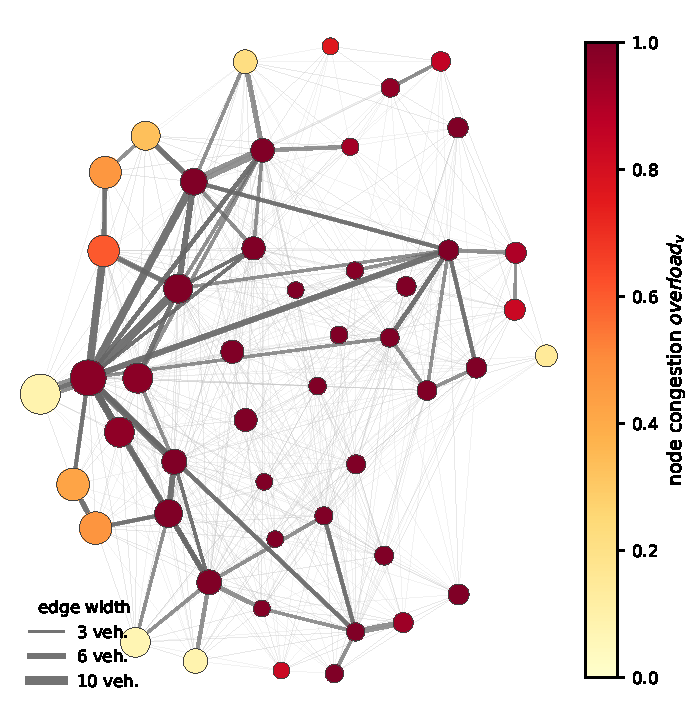
\includegraphics[height=0.46\textheight]{figs/germany_solution.pdf}

{\scriptsize Germany, $|V|=49$: a GVNS solution. Node area $=W_v$, colour $=$
congestion (dark $=$ at capacity), thick edges carry $\ge3$ vehicles.\par
\smallskip
\alert{A MIP solver given two hours returns a solution 54\% more expensive
than this one.}\par}
\end{columns}
\note{Say ``trucks'' and ``reload ceiling'', not ``MCND'' yet; say out loud
that we minimise vehicle movement cost plus reload cost. Point at the map:
thick edges are consolidated backbones, dark nodes are saturated storages. The
54\% is the ratio $1.544$ of Table~2, Germany, MIP-inc.\ column; the exact
budget at this size is 2\,h against a 98\,min limit for GVNS, of which it used
56\,min on average.}
\end{frame}

\begin{frame}{Feature 1: a road is billed per truck, not per unit}
\begin{columns}[T]
\column{0.5\textwidth}
\centering
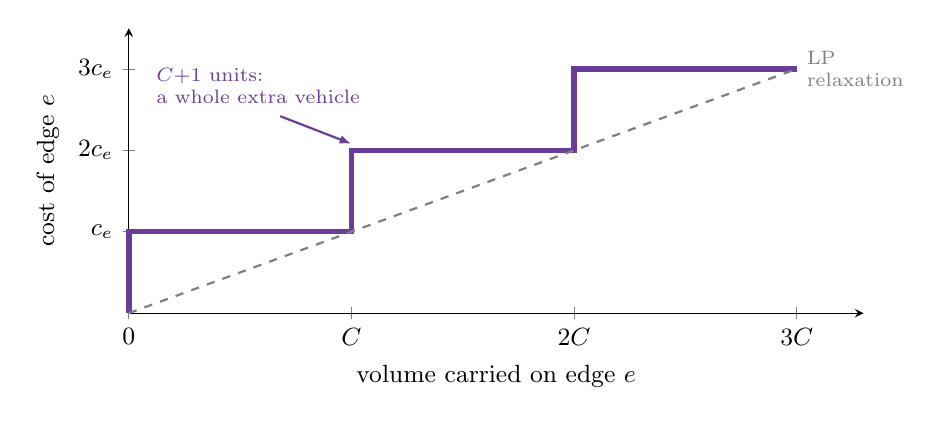
\begin{tikzpicture}
\begin{axis}[width=0.9\linewidth,height=5.2cm,xlabel={volume carried on edge $e$},ylabel={cost of edge $e$},
  xtick={0,50,100,150},xticklabels={0,$C$,$2C$,$3C$},ytick={1,2,3},yticklabels={$c_e$,$2c_e$,$3c_e$},
  ymin=0,ymax=3.5,xmin=0,xmax=165,axis lines=left,clip=false,label style={font=\small},tick label style={font=\small}]
\addplot[const plot mark right,line width=2pt,cStep] coordinates {(0,0)(0.01,1)(50,1)(50.01,2)(100,2)(100.01,3)(150,3)};
\addplot[dashed,gray,thick] coordinates {(0,0)(150,3)} node[pos=1,right,font=\scriptsize,text=gray,align=left] {LP\\relaxation};
\node[font=\scriptsize,text=cStep,align=left,anchor=south west] at (axis cs:4,2.45) {$C{+}1$ units:\\a whole extra vehicle};
\draw[-{Latex[length=1.5mm]},cStep,thick] (axis cs:34,2.42) -- (axis cs:50,2.08);
\end{axis}
\end{tikzpicture}

{\scriptsize schematic, $C=50$}
\column{0.5\textwidth}
\begin{block}{The billed quantity is the vehicle count}
\[
\text{cost of } e = \textcolor{cStep}{c_e\,y_e},\qquad y_e\in\Int_+
\]
with enough vehicles for the flow: $\sum_{k} x^k_e \le C\,y_e$
\end{block}
\begin{itemize}
\item a non-convex \emph{staircase} in the volume, shared by all requests on the edge
\item dropping integrality gives the line $c_e x/C$: the LP relaxation, polynomial but \emph{loose}
\end{itemize}
\end{columns}
\note{Practitioners recognise the staircase instantly; OR people recognise a
step-cost network design problem (Gabrel, Knippel, Minoux 1999; Croxton,
Gendron, Magnanti 2003). How loose: the LP solution with vehicles rounded up,
our starting solution, costs $1.19\times$ the GVNS solution at $|V|=10$,
$2.8\times$ at $|V|=50$ and $2.2$--$3.1\times$ at $|V|\ge90$ (Table~2).}
\end{frame}

\begin{frame}{Feature 2: every storage has a reload ceiling}
\begin{columns}[T]
\column{0.46\textwidth}
\centering
\begin{tikzpicture}[scale=0.72]
  \node[storage,minimum size=13mm,fill=cCap!60,font=\normalsize] (h) at (0,0) {$v$};
  \foreach \a/\c in {150/cN1,180/cN2,210/cOK} {\draw[flow,draw=\c] (\a:2.3) -- (h);}
  \foreach \a/\c in {30/cN1,0/cN2,-30/cOK} {\draw[flow,draw=\c] (h) -- (\a:2.3);}
  \draw[flow,draw=gray,dashed] (-2.4,-1.7) -- (-1.0,-1.0);
  \node[lbl,text=gray,align=left,anchor=north] at (-1.3,-1.85) {no room left:\\this request must detour};
  \draw[thick,mDarkTeal] (2.9,-0.9) rectangle (3.3,0.9);
  \fill[cCap!70] (2.9,-0.9) rectangle (3.3,0.9);
  \node[lbl,right] at (3.4,0.9) {$W_v$};
  \node[lbl,right,align=left] at (3.4,0.1) {transit flow\\$=W_v$};
  \node[lbl,right,text=cCap] at (3.4,-0.75) {$\ovl_v=1.0$};
\end{tikzpicture}

\medskip
{\small congestion of a storage in a solution:\\
$\ovl_v = \text{transit flow through } v\,/\,W_v$\\
$1.0$ = at capacity}
\column{0.54\textwidth}
\begin{block}{Transit volume through $v$ is bounded}
\[
\textcolor{cCap}{\sum_{k\in K:\,v\neq s_k,t_k}\ \sum_{e\in\delta^-(v)} x^k_e \;\le\; W_v}
\qquad\forall v\in V
\]
\end{block}
\begin{itemize}
\item once a storage is at capacity, further transit must detour: a longer route or a reload at a less loaded storage
\item origin and destination handling is not transshipment: a direct $s_k\!\to\!t_k$ route touches no node capacity
\end{itemize}
\end{columns}
\note{Node throughput bounds are familiar from hub location (Alumur \& Kara
2008), not from the MCND literature. $\ovl_v$ returns twice: it colours the
Germany map and it drives neighbourhood $N_3$.}
\end{frame}

\begin{frame}{Why not simply run a published network-design code?}   % [optional]
\centering
\footnotesize
\renewcommand{\arraystretch}{1.15}
\begin{tabular}{@{}l>{\raggedright\arraybackslash}p{4.6cm}>{\raggedright\arraybackslash}p{5.4cm}@{}}
\toprule
 & \textbf{fixed-charge capacitated MCND} & \textbf{this problem}\\
\midrule
arc cost & fixed charge per opened arc $+$ linear flow cost & \textcolor{cStep}{$c_e$ per vehicle: a staircase in the volume}\\
capacities & per arc & per arc (through vehicles) \textbf{and} \textcolor{cCap}{per node: transit volume $\le W_v$}\\
extra cost term & --- & reload $f_v$ per unit at every transit node\\
comparable published code & several (tabu, local branching, matheuristics) & none that we know of\\
\bottomrule
\end{tabular}

\medskip
\begin{alertblock}{Consequence for the experimental design}
no published network-design code that we know of charges per vehicle and bounds node throughput, and our open corpus has no published
objective values: we compare GVNS against \textbf{valid bounds} and \textbf{MIP solvers on the same model}
\end{alertblock}
\note{Skip in a 20-minute slot and say the consequence on the yardstick
slide. Literature, if asked (also on the backup slide ``Where it sits''):
capacitated MCND -- Gendron, Crainic, Frangioni 1999; Crainic 2000; column
generation / branch-and-price -- Barnhart et al.\ 1998; cycle-based tabu --
Ghamlouche, Crainic, Gendreau 2003; local branching -- Rodr\'iguez-Mart\'in \&
Salazar 2010; MILP-in-the-loop matheuristics -- Hewitt, Nemhauser, Savelsbergh
2010; survey -- Crainic \& Gendreau 2021. Step costs -- Gabrel, Knippel,
Minoux 1999; Croxton, Gendron, Magnanti 2003. Node capacity -- hub location,
Alumur \& Kara 2008. VNS -- Mladenovi\'c \& Hansen 1997; Hansen et al.\ 2017;
Hansen \& Mladenovi\'c 2019; multi-start VNS for single-path MCF -- Masri et
al.\ 2015; GVNS on CVRP -- Amous et al.\ 2017. Our own real-life logistic
heuristics: truck-and-trailer routing with time windows and split deliveries
(Batsyn \& Ponomarenko 2014, 2015).}
\end{frame}

% ---------------------------------------------------------------------------
\section{Model}

\begin{frame}{The model: an arc-based MILP}
\small
$x^k_e\in\Real_+$: flow of request $k$ on edge $e$;\quad
$y_e\in\Int_+$: vehicles on $e$;\quad $|K|\cdot|E|+|E|$ variables.
\vspace{-6pt}
\begin{align*}
\min\;& \textcolor{cStep}{\sum_{e\in E} c_e\,y_e}
 \;+\;\sum_{k\in K}\ \sum_{\substack{v\in V\\ v\neq s_k,t_k}}\ \sum_{e\in\delta^-(v)} f_v\,x^k_e
 &&\text{vehicles $+$ reloads}\\[-2pt]
\text{s.t.}\;&
\sum_{e\in\delta^+(v)} x^k_e-\sum_{e\in\delta^-(v)} x^k_e=
 \begin{cases} d_k & v=s_k\\ -d_k & v=t_k\\ 0 & \text{otherwise}\end{cases}
 && \forall k,\ \forall v \quad\text{(demand)}\\[-2pt]
&\textcolor{cStep}{\sum_{k\in K} x^k_e\le C\,y_e} && \forall e\in E \quad\text{(vehicle capacity)}\\
&\textcolor{cCap}{\sum_{k\in K:\,v\neq s_k,t_k}\ \sum_{e\in\delta^-(v)} x^k_e \le W_v} && \forall v\in V \quad\text{(transshipment capacity)}\\
& x\ge 0,\quad y\in\Int_+^{|E|}
\end{align*}
\vspace{-4pt}
linear objective and constraints, integer $y$, continuous $x$: a MILP, NP-hard.
This arc model is exactly what the exact solvers (HiGHS, SCIP) receive later.
\note{Read the equations once; every term was just seen in pictures. The
path-based twin has $\sum_k|\Pi_k|+|E|$ variables. Spoken bridge to the
method if the next frame is skipped: relaxing $y$ gives a per-unit path price,
travel$/C$ plus one reload per transit node, so the relaxation wants cheap
transit-free paths; that is why the start solution is every request on its
direct edge, and why $N_1$ searches with a reload-aware metric.}
\end{frame}

\begin{frame}{Path form, and what the LP relaxation tells us}   % [optional]
\begin{columns}[T]
\column{0.6\textwidth}
\textbf{Path form.} Flow $x^k_p$ on paths $p\in\Pi_k$ (all $s_k\!\to\!t_k$ paths),
$\sum_{p\in\Pi_k}x^k_p=d_k$, same $y_e$; only the paths that carry flow matter.

\medskip
\textbf{Relax integrality.} The capacity constraint becomes tight, so
$y_e=\frac1C\sum_k\sum_{p\ni e}x^k_p$ and $y$ disappears:
\[
\min\ \sum_{k\in K}\sum_{p\in\Pi_k} x^k_p\;
\underbrace{\Bigg(\frac1C\sum_{e\in p} c_e+\sum_{\substack{v\in p\\ v\neq s_k,t_k}} f_v\Bigg)}_{\text{per-unit price of path } p}
\]
\column{0.4\textwidth}
\centering
\begin{tikzpicture}
  \node[storage] (s) at (0,0) {$s$};
  \node[storage,fill=cCap!30] (v) at (2,0.9) {$v$};
  \node[storage] (t) at (4,0) {$t$};
  \draw[flow] (s) -- node[lbl,above left] {$c_{sv}/C$} (v);
  \draw[flow] (v) -- node[lbl,above right] {$c_{vt}/C$} (t);
  \node[lbl,text=cCap,above=1mm of v] {$+\,f_v$};
  \draw[road,dashed] (s) -- node[lbl,below] {$c_{st}/C$, no reload} (t);
\end{tikzpicture}

\medskip
\begin{block}{Reading}
a unit of flow pays \emph{travel}$/C$ plus one reload per transit node: the relaxation prefers cheap, transit-free paths
\end{block}
\end{columns}
\medskip
\begin{itemize}
\item on the completed graph the relaxed optimum puts every request on its direct edge: our \textbf{starting solution}; the search metric of $N_1$ is an edge-wise version of this price
\end{itemize}
\note{Bridge from model to method; skip in a 20-minute slot (the model frame's
note has the spoken version). $N_1$'s metric $c'_{vu}=f_v+f_u+c_{vu}/C$ is
edge-wise, so a transit reload is charged on both incident edges; it is a
ranking metric for path generation, not the objective---the MILP prices every
path exactly.}
\end{frame}

% ---------------------------------------------------------------------------
\section{The GVNS}

\begin{frame}{GVNS at a glance}
\centering
\begin{tikzpicture}[node distance=5mm and 6mm, box/.append style={text width=2.75cm,font=\scriptsize}]
  \node[box] (init) {\textbf{initial solution}\\rounded LP:\\every request on its direct edge};
  \node[box,right=of init,fill=cN2!15] (shake) {\textbf{Shake} in $N_k$\\diversified\\random paths\\MILP budget $\tau_{\mathrm{shk}}$};
  \node[box,right=11mm of shake,fill=cN1!15] (vnd) {\textbf{VND} $N_1\!\to\!N_2\!\to\!N_3$\\restart at $N_1$ on improvement\\MILP budget $\tau_{\mathrm{vnd}}$};
  \node[box,right=of vnd,text width=1.6cm] (test) {$z<z_0$?};
  \draw[road] (init) -- (shake);
  \draw[road] (shake) -- node[lbl,above=2pt,font=\scriptsize] {$z_0\gets z$} (vnd);
  \draw[road] (vnd) -- (test);
  \draw[road,draw=cOK] (test.south) -- ++(0,-0.55) -| node[pos=0.25,below,font=\scriptsize,text=cOK] {yes: $k\gets1$} (shake.south);
  \draw[road,draw=cN3] (test.south) -- ++(0,-1.15) -| node[pos=0.25,below,font=\scriptsize,text=cN3] {no: $k\gets k+1$} ($(shake.south)+(-0.5,0)$);
\end{tikzpicture}

\medskip
\begin{itemize}
\item \textbf{search space: commodity paths.} A solution is a path pool $P$ with flows $x$; vehicle counts follow, $y_e=\big\lceil\frac1C\sum_k x^k_e\big\rceil$
\item \textbf{shake and VND are the same primitive} (next slide): the shake adds more, random paths with a larger MILP budget
\item \textbf{stop} when $k>3$ or after $t_{\max}=2|V|$ minutes; a move is accepted \emph{only if it improves}, so the shake never degrades the incumbent, and $k$ advances when the VND fails to beat the post-shake value $z_0$
\end{itemize}
\note{Preprocessing: complete the graph, build the reload-aware graph $G'$,
precompute 20 shortest paths per request. Shake vs VND path counts: 5 random
pool paths vs 1--3 for $N_1$; stop at 3 fully loaded paths / $5C$ free room vs 2 / $1C$ for $N_2$;
3 detours vs 1 for $N_3$. Budgets: $\tau_{\mathrm{shk}}=10+|V|$ / $100+2|V|$\,s,
$\tau_{\mathrm{vnd}}=25$ / $70$\,s ($N_1$ / rest; 15 / 50\,s at $|V|=100$), so
for $N_1$ the shake budget is smaller than the VND budget while $|V|\le14$.
A VNS-school listener will ask whether this is a shake: it is Algorithm~1
called with diversified generation and $\tau_{\mathrm{shk}}$; diversification
comes from the random paths pushed into the pool and the MILP re-optimisation,
and a non-improving shake is discarded. All parameters are on the backup slide
``Settings''.}
\end{frame}

\begin{frame}{Preprocessing and the starting solution}   % [optional]
\begin{columns}[T]
\column{0.5\textwidth}
\centering
\begin{tikzpicture}[scale=0.68]
  \node[storage] (a) at (0,0) {$a$};
  \node[storage] (b) at (1.6,1.2) {$b$};
  \node[storage] (c) at (3.2,0.2) {$c$};
  \node[storage] (d) at (1.8,-1.2) {$d$};
  \draw[road] (a) -- (b); \draw[road] (b) -- (c); \draw[road] (a) -- (d); \draw[road] (d) -- (c);
  \node[lbl,text=black] at (1.6,-2.0) {(a) raw road graph};
  \begin{scope}[xshift=6.0cm]
  \node[storage] (a2) at (0,0) {$a$};
  \node[storage] (b2) at (1.6,1.2) {$b$};
  \node[storage] (c2) at (3.2,0.2) {$c$};
  \node[storage] (d2) at (1.8,-1.2) {$d$};
  \draw[road] (a2) -- (b2); \draw[road] (b2) -- (c2); \draw[road] (a2) -- (d2); \draw[road] (d2) -- (c2);
  \draw[road,dashed,draw=cN1] (a2) -- node[lbl,text=cN1,above,pos=0.78] {$c_{ac}$} (c2);
  \draw[road,dashed,draw=cN1] (b2) -- (d2);
  \node[lbl,text=black] at (1.6,-2.0) {(b) completed graph};
  \end{scope}
\end{tikzpicture}
\column{0.5\textwidth}
\begin{itemize}
\item road graphs are sparse ($a\!\to\!c$ needs a stop); on the raw graph a missing origin--destination path can even make an instance infeasible
\item \textbf{completion}: join every ordered pair by an edge costing the shortest path in $G$ ($c_{ac}$): the cheapest \emph{stop-free} route, touching no $W_v$
\item the exact solvers get the same completed graph ($|E|=|V|(|V|-1)$)
\end{itemize}
\end{columns}
\smallskip
\begin{block}{Start: the rounded LP}
every request on its direct edge (the relaxed optimum), vehicles rounded up: always feasible, and poor ($1.19\times$ GVNS at $|V|=10$, $2.80\times$ at 50, $3.14\times$ on European Russia)
\end{block}
\note{Skip in a 20-minute slot: say ``we complete the graph so every request
has a direct stop-free edge, and start from the rounded LP''. On the raw graph
the node capacities also shrink the feasible region (paper, Sec.~3.2). Many of the
trucks on those direct edges leave partly empty---that is what $N_2$ will fix.
The initial MILP that sets up the flows has a 300\,s limit.}
\end{frame}

\begin{frame}{The move primitive: propose paths, let the MILP redistribute}
\centering
\begin{tikzpicture}[node distance=5mm]
  \node[box,fill=cN1!10] (gen) {\textbf{GenPaths}$(N,k)$\\new candidate paths $Q$\\for every request $k$};
  \node[box,right=of gen] (milp) {\textbf{MILP} on pool $P\cup Q$\\redistribute flow: warm start $x$,\\time limit $\tau$, gap 1\%};
  \node[box,right=of milp,fill=cOK!10] (keep) {improved ($z'<z$)?\\keep new paths with $x'_p>0$,\\prune every zero-flow path};
  \node[box,below=3mm of keep,fill=cCap!10,text width=3.6cm] (drop) {not improved: discard $Q$};
  \draw[road] (gen) -- (milp);
  \draw[road] (milp) -- (keep);
  \draw[road] (milp.east) -- ++(0.35,0) |- (drop.west);
\end{tikzpicture}

\medskip
\begin{columns}[T]
\column{0.5\textwidth}
\begin{block}{Why paths and not edge flows}
per-edge flows are strongly coupled across requests, so a feasible change needs the whole network at once; a path describes one request only, and \emph{adding} a path to a feasible solution never makes it worse
\end{block}
\column{0.5\textwidth}
\begin{itemize}
\item the three neighbourhoods differ \emph{only} in \textbf{GenPaths}; everything else is shared
\item pruning zero-flow paths keeps the in-loop MILP small enough for budgets of 25--70\,s (VND) and $10{+}|V|$ to $100{+}2|V|$\,s (shake)
\item the neighbourhood proposes, the MILP disposes
\end{itemize}
\end{columns}
\note{This is the matheuristic core; OR people will map it to MILP-in-the-loop
schemes (Hewitt et al.). The MILP is HiGHS with a 1\% gap target.}
\end{frame}

\begin{frame}{\textcolor{cN1}{$N_1$}: reload-aware shortest paths}
\begin{columns}[T]
\column{0.45\textwidth}
\centering
\begin{tikzpicture}[scale=1.15]
  \node[storage] (s) at (0,0) {$s$};
  \node[storage,fill=cCap!30] (h) at (2.2,1.1) {$h$};
  \node[storage] (t) at (4.4,0) {$t$};
  \draw[road,draw=cN1,line width=1.5pt] (s) -- node[lbl,above left,text=cN1] {$c'_{sh}$} (h);
  \draw[road,draw=cN1,line width=1.5pt] (h) -- node[lbl,above right,text=cN1] {$c'_{ht}$} (t);
  \draw[road,draw=cN1,line width=1.5pt] (s) -- node[lbl,below,text=cN1] {$c'_{st}$} (t);
  \foreach \i in {1,...,6} {\draw[cN1!30,line width=0.6pt] (0.2,-0.9-0.13*\i) -- (3.0,-0.9-0.13*\i);}
  \foreach \i in {1,2,3} {\draw[cN1,line width=1pt] (0.2,-0.9-0.13*\i) -- (3.0,-0.9-0.13*\i);}
  \node[lbl,right,text=cN1,align=left] at (3.1,-1.35) {pool of 20 paths\\per request};
\end{tikzpicture}
\column{0.55\textwidth}
\begin{block}{Auxiliary complete graph $G'$: per-unit weights}
\[
c'_{vu}=f_v+f_u+\frac{c_{vu}}{C}\qquad\forall (v,u)\in E
\]
travel per unit plus the reloads at the endpoints; plain shortest paths would ignore the reloads
\end{block}
\begin{itemize}
\item 20 shortest paths per request under $c'$, precomputed once; new paths come from this pool
\item \textbf{VND}: $\{1,2,3\}$ new paths per request $\times$ \{random, low-cost first\}; \textbf{Shake}: 5 random pool paths
\item ablation: without $N_1$, $+0.8\%$ (median, synthetic and real alike)
\end{itemize}
\end{columns}
\note{Keep short: $N_2$ is where the money is. If a sharp listener notes that
$c'$ charges a transit reload on both incident edges and also prices origin
and destination reloads: $c'$ is a ranking metric for path generation, not the
objective; the MILP prices every path exactly, so the double count only changes
which 20 paths enter the pool.}
\end{frame}

\begin{frame}{\textcolor{cN2}{$N_2$}: fill the half-empty trucks}
\begin{columns}[T]
\column{0.46\textwidth}
\centering
\begin{tikzpicture}[x=1cm,y=1cm,scale=0.8]
  \node[font=\footnotesize] at (2.7,1.35) {edge $(u,v)$: 110 units, $y_{uv}=\lceil 110/50\rceil=3$};
  \foreach \i/\l in {0/50, 1/50, 2/10} {
    \draw[thick,mDarkTeal] (\i*1.9,0) rectangle ++(1.6,0.7);
    \fill[cN1!60] (\i*1.9,0) rectangle ++(1.6*\l/50,0.7);
    \node[font=\scriptsize] at (\i*1.9+0.8,-0.3) {\l\,/\,50};
  }
  \draw[{Latex}-{Latex},cN2,line width=1.5pt] (3.8+0.33,0.35) -- (3.8+1.58,0.35);
  \node[font=\scriptsize,text=cN2,align=center] at (4.75,0.95) {40 units free};
  \node[font=\footnotesize,align=center] at (2.7,-1.15) {$\load_{uv}=110 \bmod 50 = 10$:\\up to 40 more units here cost \textbf{no extra vehicle}\\and may free one elsewhere};
\end{tikzpicture}

\medskip
\begin{itemize}
\item shortest paths on $G''$ run through partially loaded vehicles
\item dynamic number of new paths per request: stop after 2 fully loaded paths or accumulated free room $\ge1C$ (VND); 3 fully loaded paths or $\ge5C$ (Shake)
\end{itemize}
\column{0.54\textwidth}
\begin{block}{Graph $G''$ favours free room ($\alpha=0.5$)}
\small
\begin{gather*}
c''_{vu}=f_v+f_u+\frac{\load_{vu}}{C}\Big(\frac{c_{vu}}{C}\Big)^{\!\alpha}\\[-2pt]
\load_e=\Big(\textstyle\sum_k\sum_{p\ni e}x^k_p\Big)\bmod C
\end{gather*}
fully loaded edges ($\load_e=0$) keep their $G'$ weight; smaller residual load $\Rightarrow$ lower weight
\end{block}
\begin{alertblock}{Ablation: the dominant operator}
without $N_2$: $+3.9\%$ synthetic, $+1.6\%$ real (medians), up to $+23.8\%$ on a single instance
\end{alertblock}
\end{columns}
\note{Slow down here. Vehicle consolidation is the main lever on the
objective. On the synthetic ablation subset the mean loss is $+7.1\%$ and the
worst case $+23.8\%$ (50\_nodes\_2); on the real subset the mean is $+2.6\%$
and Germany loses $7.6\%$ (components\_A.csv); none of these is corpus-wide.}
\end{frame}

\begin{frame}{\textcolor{cN3}{$N_3$}: detour around the saturated storage}
\begin{columns}[T]
\column{0.48\textwidth}
\centering
\begin{tikzpicture}
  \node[storage] (a) at (0,0) {$s$};
  \node[storage,minimum size=10mm,fill=cCap!70] (b) at (2.4,0) {$v^\ast$};
  \node[storage] (c) at (4.8,0) {$t$};
  \node[storage,fill=cN1!20] (d) at (2.4,-1.6) {$w$};
  \draw[road] (a) -- (b); \draw[road] (b) -- (c);
  \draw[cCap,line width=1.5pt] (b.north west) -- (b.south east); \draw[cCap,line width=1.5pt] (b.north east) -- (b.south west);
  \draw[flow] (a) to[bend right=25] (d); \draw[flow] (d) to[bend right=25] (c);
  \node[lbl,text=cCap,above=1.5mm of b] {$\ovl_{v^\ast}\approx1$: removed from $G'$};
  \node[lbl,below=1mm of d] {new shortest path through a less loaded $w$};
\end{tikzpicture}

\medskip
{\small in the current solution:\\[2pt]
$\ovl_v=\dfrac1{W_v}\displaystyle\sum_{k:\,v\neq s_k,t_k}\ \sum_{p\in\Pi_k:\,v\in p}x^k_p$}
\column{0.52\textwidth}
\begin{itemize}
\item delete the \textbf{single most congested} storage from $G'$ (unless it is the request's own origin or destination), recompute the shortest path: a detour to less loaded storages
\item 1 new path per request in VND, 3 in Shake
\item ablation: $+0.1\%$ / $+0.2\%$ median, \textbf{inactive when capacities are slack}; $+4.0\%$ on Germany, where almost every storage runs at capacity
\end{itemize}
\end{columns}
\note{Say ``situational'' out loud: the operator is worth carrying only for
tight instances---when capacities are slack there is nothing to route around.
Point back at the Germany map. If asked why a single node: removing a prefix
of $|V|/5$--$|V|/4$ congested storages was tried on all 50 instances $\times$
10 seeds; it is indistinguishable on 44 of 50 (within across-seed noise) yet
forfeits $N_3$'s benefit on the capacity-tight networks, so the surgical
version is kept---state the measured outcome, not a mechanism.}
\end{frame}

% ---------------------------------------------------------------------------
\section{Experiments}

\begin{frame}{The benchmark: realistic regional networks, openly available}
\begin{columns}[T]
\column{0.56\textwidth}
\begin{itemize}
\item our open corpus (arXiv:2606.20653; Zenodo, CC-BY-4.0), every instance reproducible from its published seed
\item road networks between regional sorting centres, calibrated on OpenStreetMap for \textbf{nine European countries, five U.S.\ states and European Russia}
\item real structure: Zipf city sizes, spatial-network topology, centrality-driven $W_v$, gravity demand; near-planar, large-diameter graphs
\item \textbf{35 synthetic}: $10\times|V|{=}10$, $7\times20$, $7\times30$, $5\times50$, $3\times100$, $3\times150$
\item \textbf{15 real-geometry}: Denmark ($|V|=11$) to European Russia ($|V|=90$)
\end{itemize}
\column{0.44\textwidth}
\centering
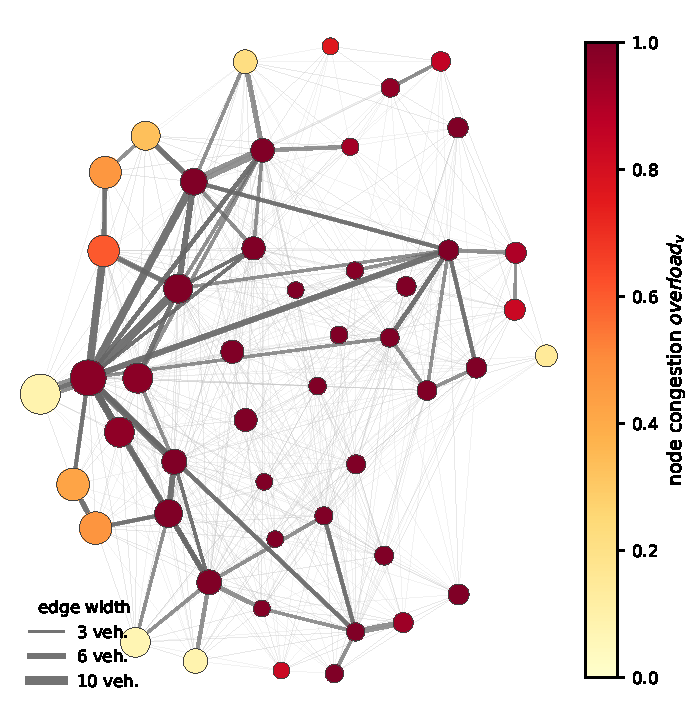
\includegraphics[height=0.52\textheight]{figs/germany_solution.pdf}

{\scriptsize Germany ($|V|=49$), the solution from the first slide:
almost every storage runs at capacity.\par}
\end{columns}
\note{The generator is a separate paper; here only what the study needs.
Mean degree is 3.575 in the paper. Point at the map: thick edges are
consolidation ($N_2$) made visible, dark nodes are what $N_3$ works on. The
instance's numbers come where they are defined: $\gapLB=11.0\%$, exact
incumbent $1.544\times$, rounded-LP start $2.692\times$, $\sigma$ over 10 seeds
$2.0\%$; without $N_2$ $+7.6\%$, without $N_3$ $+4.0\%$.}
\end{frame}

\begin{frame}{Setup and yardsticks}
\centering
\begin{tikzpicture}[x=1cm]
  \draw[-{Latex[length=2.5mm]},thick,mDarkTeal] (0,0) -- (13.2,0) node[right,font=\scriptsize] {objective};
  \foreach \x/\lab/\val/\col in {0.9/{LP relaxation}/{0.971}/gray, 3.6/{MIP dual bound $\underline{z}$}/{}/cN1, 6.2/{optimum $z^\ast$}/{(unknown)}/gray, 8.8/{GVNS}/{1.0}/mLightBrown, 11.8/{rounded LP (start)}/{1.192}/gray}{
    \draw[thick,\col] (\x,-0.15) -- (\x,0.15);
    \node[font=\scriptsize,text=\col,align=center,above=1mm] at (\x,0.15) {\lab\\ \val};
  }
  \node[font=\scriptsize,text=cOK,align=center,below=1mm] at (8.8,-0.15) {MIP incumbent 1.000};
  \draw[{Bar}-{Bar},thick,cN1] (3.6,-0.75) -- (8.8,-0.75) node[midway,below,font=\scriptsize,text=cN1] {$\gapLB=0.96\%$};
  \node[font=\scriptsize,text=gray] at (11.8,-0.8) {ratios: means at $|V|=10$; not to scale};
\end{tikzpicture}

\smallskip
\begin{columns}[T]
\column{0.48\textwidth}
\begin{block}{Two metrics}
\small
$\gapLB=\big(\mathit{Result}_{\mathrm{GVNS}}-\underline{z}\big)/\underline{z}$,\quad $\underline{z}=$ best MIP dual bound:
an \textbf{upper bound on the true optimality gap} of GVNS\\[3pt]
$\mathit{Ratio}_{\mathrm{method}}=\mathit{Result}_{\mathrm{method}}/\mathit{Result}_{\mathrm{GVNS}}$:
below 1 better than GVNS, above 1 worse
\end{block}
\column{0.52\textwidth}
\begin{itemize}\small
\item GVNS: 10 seeds per instance, limit $2|V|$\,min; exact: gap target 0, 30\,min--4\,h, i.e.\ comparable budgets ($|V|=50$: 100\,min vs 2\,h); HiGHS is the exact baseline \emph{and} the in-loop solver
\item nothing is proven optimal, but $\underline{z}$ is a valid lower bound, typically within a few percent of the incumbent: $\gapLB$ is a guarantee, not a self-comparison
\end{itemize}
\end{columns}
\note{Hardware: HSE cluster cHARISMa, nodes with 2$\times$AMD EPYC (44 cores,
$\ge$720\,GB RAM), each job pinned to 8 cores; HiGHS 1.14.0, SCIP 10.0.2 as
cross-check. Exact side in one breath: none of the 50 instances was solved to
proven optimality; up to $|V|=42$ the two solvers' dual bounds agree within
$0.6\%$; SCIP returns nothing usable from $|V|=45$; the arc model is out of
memory at $|V|\ge100$ (backup ``The exact side''). If you accept one number
from this talk, make it $\gapLB$: it bounds the distance to the optimum instead
of comparing GVNS with itself. The ladder ticks are the $|V|=10$ means of
Table~2; the dual bound sits between the LP and GVNS, and GVNS is $0.96\%$
above it.}
\end{frame}

\begin{frame}{Results I: synthetic instances}
\begin{columns}[T]
\column{0.56\textwidth}
\centering
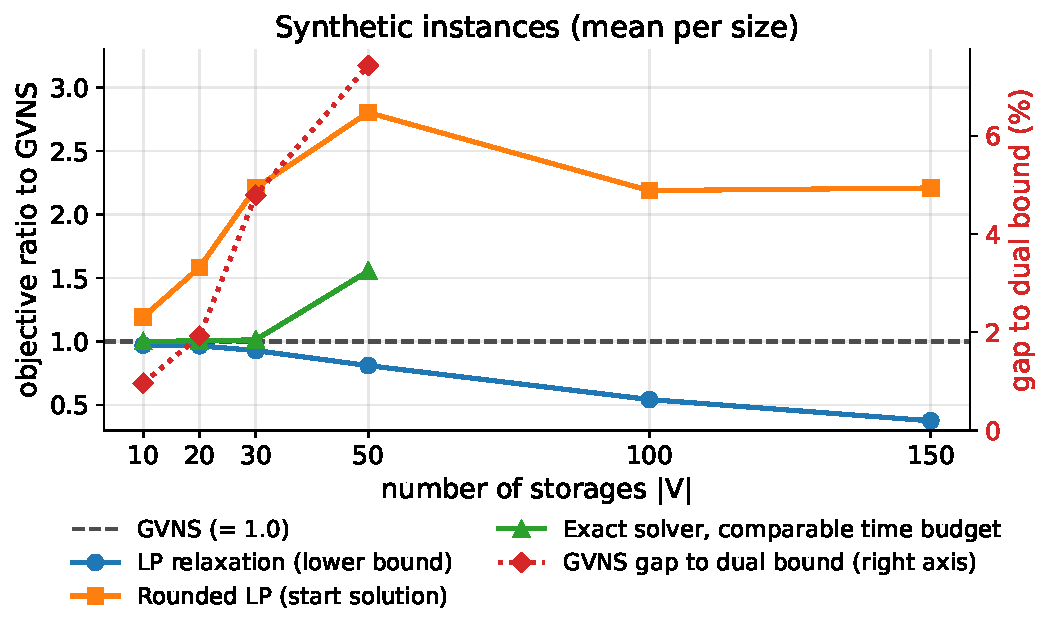
\includegraphics[width=0.94\linewidth]{figs/ratios_synthetic.pdf}
\column{0.44\textwidth}
\centering
\small
\setlength{\tabcolsep}{4pt}
\begin{tabular}{@{}rrccc@{}}
\toprule
$|V|$ & $n$ & $\gapLB$ & exact inc. & $\sigma$\\
\midrule
10  & 10 & 0.96\% & 1.000 & 0.06\%\\
20  & 7  & 1.92\% & 1.005 & 0.18\%\\
30  & 7  & 4.79\% & 1.013 & 0.68\%\\
50  & 5  & 7.44\% & \alert{1.555} & 0.66\%\\
100 & 3  & \dag & \dag & 0.31\%\\
150 & 3  & \dag & \dag & 0.38\%\\
\bottomrule
\end{tabular}

{\scriptsize\dag: arc model intractable; only the loose LP bound (0.542, 0.375)\par}

\smallskip
{\small near-optimal up to $|V|=20$; at $|V|=50$ the exact solver with a comparable budget is \alert{55\% more expensive} on average (16\% to 137\% per instance)\par}
\end{columns}
{\scriptsize GVNS mostly stops before its limit (3\,729 of 6\,000\,s at $|V|=50$); the exact solver always used its full budget, so the comparison is conservative.\par}
\note{Trace the green curve: flat at 1.0, up to 1.555 at 50, then it stops
existing. Spoken: $\gapLB$ is about 1--2\% up to $|V|\approx20$, 4.8\% at 30,
7.4\% at 50, where the LP bound alone would say about 24\%; at $|V|\ge100$
GVNS still ends $2.2\times$ below its own start. Mean run time vs limit:
633/1\,200\,s (10), 1\,952/2\,400 (20), 2\,611/3\,600 (30), 3\,729/6\,000 (50),
5\,983/12\,000 (100), 18\,236/18\,000 (150); the 150-node mean slightly exceeds
its limit because Algorithm~2 tests $t_{\max}$ only before each shake and after
each full VND sweep, so a shake started just under the limit (MILP budget up to
$100+2|V|=400$\,s at $|V|=150$) and the sweep after it run to completion.
Per-instance $|V|=50$ numbers are on the backup slide ``What the means hide''.}
\end{frame}

\begin{frame}{Results II: real road geometries mirror the synthetic story}
\begin{columns}[T]
\column{0.58\textwidth}
\centering
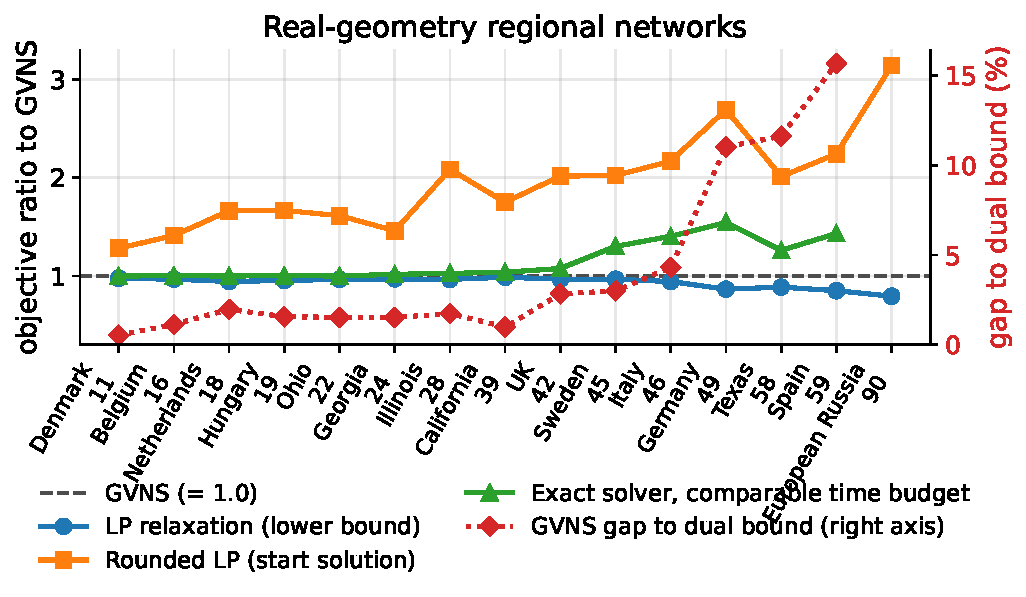
\includegraphics[width=\linewidth]{figs/ratios_real.pdf}
\column{0.42\textwidth}
\begin{itemize}
\item exact solver with a comparable budget: parity up to $|V|=22$, $1.02$--$1.08\times$ up to the UK (42), then \alert{$1.26$--$1.54\times$} from Sweden (45) to Spain (59)
\item $\gapLB$ from $0.5\%$ (Denmark, 11) to $15.7\%$ (Spain, 59)
\item European Russia ($|V|=90$): no exact reference; GVNS ends $3.1\times$ below its start
\end{itemize}
\medskip
{\small\itshape same shape as the synthetic curves: the synthetic corpus behaves like the real geometries, and GVNS is robust to them}
\end{columns}
\note{Do not read the table; point at the three medium networks and at the
90-node one. Spoken detail: $\gapLB$ about 1--3\% up to $|V|=45$, 4.3\% on
Italy (46), 11.0\% Germany (49), 11.6\% Texas (58), 15.7\% Spain (59); exact
incumbent 1.02--1.04$\times$ from Georgia (24) to California (39), 1.077 UK;
run time 615\,s (Denmark) to 3\,986\,s (Spain), 5\,595\,s on European Russia.
Full Table~2 rows are in the paper.}
\end{frame}

\begin{frame}{How many seeds do you need?}   % [optional]
\begin{columns}[T]
\column{0.58\textwidth}
\centering
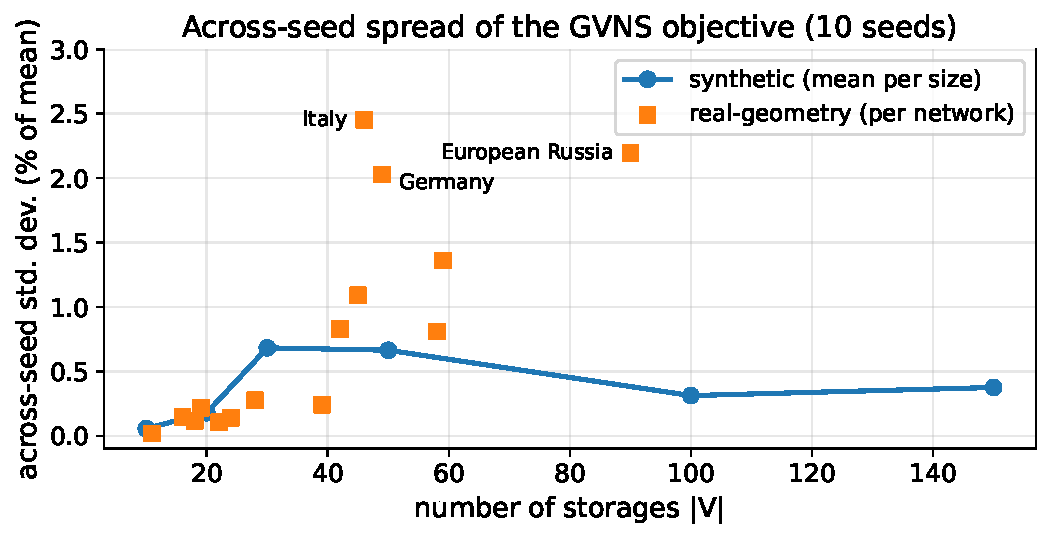
\includegraphics[width=\linewidth]{figs/seed_spread.pdf}
\column{0.42\textwidth}
\begin{itemize}
\item synthetic: across-seed $\sigma$ below $0.7\%$ of the mean at every size, below $0.2\%$ up to $|V|=20$
\item large real networks: $2.0\%$ (Germany), $2.5\%$ (Italy), $2.2\%$ (European Russia)
\item \alert{three seeds badly understate it}: on Italy the spread over three seeds is $0.4\%$ against $2.5\%$ over ten
\item one run is representative on small networks; on capacity-tight instances take the best of several
\end{itemize}
\end{columns}
\note{Backup for the ``is it stable?'' question. We moved from 3 to 10 seeds
for the headline numbers and 5 for the component study.}
\end{frame}

\begin{frame}{What each component buys}
\begin{columns}[T]
\column{0.54\textwidth}
\centering
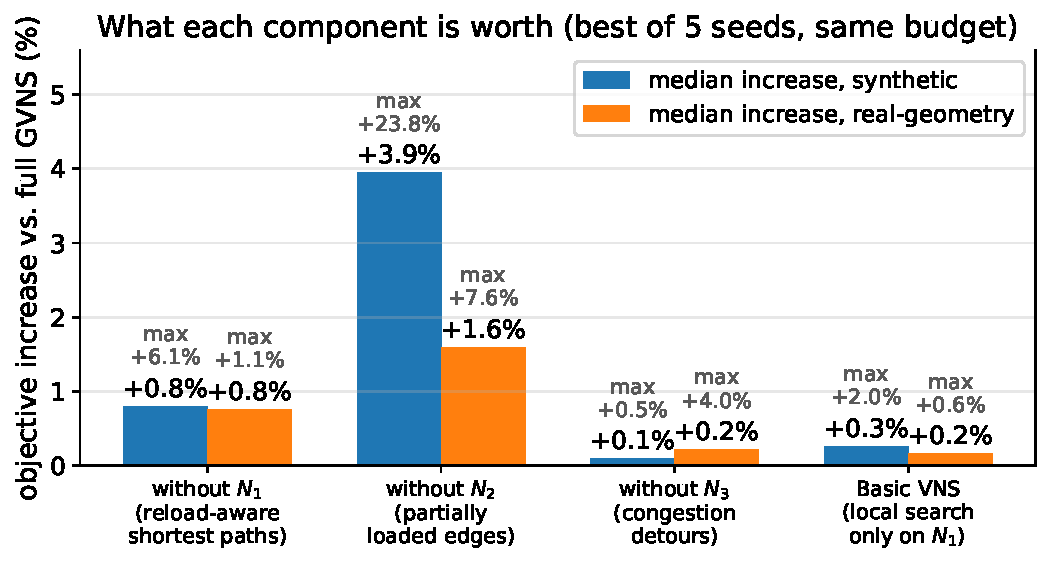
\includegraphics[width=\linewidth]{figs/ablation.pdf}

{\scriptsize best of 5 seeds, same budget, subset of synthetic ($|V|=20$--$100$) and real ($16$--$49$) instances; medians because the seed spread is heavy-tailed on capacity-tight networks\par}
\column{0.46\textwidth}
\footnotesize
\setlength{\tabcolsep}{3pt}
\begin{tabular}{@{}lcc@{}}
\toprule
GVNS better / tie / variant better & synth. & real\\
\midrule
without $N_1$ & 8 / 0 / 1 & 5 / 1 / 0\\
without $N_2$ & 8 / 1 / 0 & 5 / 1 / 0\\
without $N_3$ & 1 / 8 / 0 & 3 / 3 / 0\\
Basic VNS & 5 / 4 / 1 & 2 / 4 / 0\\
\bottomrule
\end{tabular}

{\scriptsize ``decided'' = difference beyond the seed spread of both runs; time relative to GVNS: 0.80, 0.52, 0.68, 0.63\par}

\medskip
\begin{itemize}\small
\item \textcolor{cN2}{$N_2$ dominates}; \textcolor{cN3}{$N_3$ is situational}: ties when capacities are slack, $+4.0\%$ on Germany
\item \textbf{Basic VNS} (local search on $N_1$ only, same shake): GVNS better on 7 of 16, Basic VNS on 1, 8 ties; the margin grows with size, $0.2$--$0.6\%$ at $|V|\le28$ vs $1.1$--$2.0\%$ at $|V|\ge50$, for $1/0.63$ of the time
\end{itemize}
\end{columns}
\note{One line: $N_2$ dominates, the VND matters at scale, $N_3$ is for tight
instances. Table~3's time ratios are the means of the synthetic and real
groups (CSV: $N_1$ 0.76/0.84, $N_2$ 0.54/0.50, $N_3$ 0.73/0.63, Basic VNS
0.68/0.58). The CSV's \texttt{argmax\_instance} names the instance where the
variant is \emph{worst}, not best. Single instances can flip sign: the two
``variant better'' entries in the table are decided (beyond the seed spread of
both runs): 50\_nodes\_2, where dropping $N_1$ improved the result by 2.1\%, and
30\_nodes\_2, where Basic VNS beat GVNS by 1.3\%; Basic VNS also improves
Germany by 4.0\%, but inside its 4.2\% seed spread there, so a tie.}
\end{frame}

% ---------------------------------------------------------------------------
\section{Closing}

\begin{frame}{Limitations, and what comes next}
\begin{columns}[T]
\column{0.5\textwidth}
\textbf{Stated before you ask}
\begin{itemize}\small
\item \textbf{static capacities and costs}: on real networks they vary with the time of day
\item \textbf{no proven optima}: $\gapLB$ is an upper bound on the true gap
\item \textbf{no tight reference beyond $|V|=59$}: only the loose LP bound
\item \textbf{path generation is heuristic}: a pool of 20 shortest paths plus three rules
\item \textbf{open-source solvers at default settings} as the exact baseline (tuning checked on 8 instances)
\item \textbf{component study} on a subset with five seeds; \textbf{no operational data} yet
\end{itemize}
\column{0.5\textwidth}
\textbf{Next}
\begin{itemize}\small
\item time-expanded graph with period-dependent $C_e(t)$, $W_v(t)$: the neighbourhoods only need a period-aware edge metric
\item column-generation pricing to feed the path pool
\item validation on operational data
\end{itemize}
\end{columns}
\note{Justifications, spoken: at $|V|=50$--$59$ the 7--16\% gap cannot be split
between heuristic error and bound weakness; beyond $|V|=59$ the LP bound is
0.795 on European Russia and 0.542 / 0.375 at 100 / 150; HiGHS and SCIP with
three presets each moved nothing (backup ``The exact side''). The ``next''
items answer the first, fourth and last limitations.}
\end{frame}

\begin{frame}{Takeaways}
\begin{enumerate}\setlength{\itemsep}{8pt}
\item \textcolor{cStep}{integer trucks} $+$ \textcolor{cCap}{reload ceilings}: compare against \textbf{valid dual bounds}, not fixed-charge codes
\item path-space GVNS: within $\approx1\%$ of the dual bound on small networks; the exact solver is \textbf{up to 55\% more expensive} at $|V|=50$
\item \textcolor{cN2}{$N_2$} is the lever, \textcolor{cN3}{$N_3$} only when capacity binds, the full VND pays at scale
\end{enumerate}
\bigskip
\begin{center}
{\large\itshape Let cheap path generators propose and a time-boxed MILP dispose:\\
$N_2$ always, $N_3$ when capacity binds, the full VND once the network is large.}
\end{center}
\note{End on the italic sentence; it calls back to ``the neighbourhood
proposes, the MILP disposes'' on the primitive slide.}
\end{frame}

\begin{frame}{Thank you}
\begin{columns}[T]
\column{0.58\textwidth}
\textbf{Code, exact-solver harness, scripts that regenerate every table and figure}\\
{\small\href{https://github.com/aponom84/Optimal-Logistic-Net}{\texttt{github.com/aponom84/Optimal-Logistic-Net}}}

\medskip
\textbf{Instance corpus} (CC-BY-4.0)\\
{\small\href{https://doi.org/10.5281/zenodo.20372456}{\texttt{doi.org/10.5281/zenodo.20372456}}}

\medskip
\textbf{Contact}\\
\texttt{aponomarenko@hse.ru} $\cdot$ \texttt{varvara\_kovaleva03@mail.ru}

\bigskip
{\footnotesize Supported by the Basic Research Program at HSE University
(HSE-BR-2025-080) and by the HPC facilities of HSE University (cHARISMa).\par}
\column{0.42\textwidth}
\centering
\begin{tabular}{c@{\hspace{6mm}}c}
\qrcode[height=2.4cm]{https://github.com/aponom84/Optimal-Logistic-Net} &
\qrcode[height=2.4cm]{https://doi.org/10.5281/zenodo.20372456}\\[3pt]
{\small code} & {\small data}
\end{tabular}
\end{columns}
\note{Question map: seeds -- ``How many seeds''; solver behaviour and tuning --
backup ``The exact side''; per-instance spread at $|V|=50$ -- backup ``What
the means hide''; any parameter -- backup ``Settings''; literature -- backup
``Where it sits''; the $N_3$ prefix variant -- the $N_3$ slide's note.}
\end{frame}

% ---------------------------------------------------------------------------
% Backup slides: no progress bar (its denominator is the appendix frame
% count, which appendixnumberbeamer only knows after the first pass).
\appendix
\metroset{progressbar=none}

\begin{frame}{Backup: settings (Table~1 of the paper)}
\centering
\small
\renewcommand{\arraystretch}{1.15}
\setlength{\tabcolsep}{4pt}
\begin{tabular}{llll}
\toprule
Setting & Value & Setting & Value\\
\midrule
neighbourhoods $k_{\max}$ & 3 & $N_2$ exponent $\alpha$ & 0.5\\
GVNS limit $t_{\max}$ & $2|V|$\,min & $N_2$ free-room stop & $1C$ / $5C$\\
random seeds & 10 / 5 (components) & $N_3$ storages removed & 1 (most congested)\\
vehicle capacity $C$ & 50 & $N_1$ path pool & 20\\
$N_1$ paths per request & 1--3 / 5 & $N_3$ paths per request & 1 / 3\\
initial MILP limit & 300\,s & exact gap target & 0\\
redistribution MILP gap & 1\% & exact budget & 30\,min--4\,h\\
$\tau_{\mathrm{shk}}$ ($N_1$ / rest) & $10{+}|V|$ / $100{+}2|V|$\,s & $\tau_{\mathrm{vnd}}$ ($N_1$ / rest) & 25 / 70\,s ($15$ / $50$\,s at $|V|=100$)\\
\bottomrule
\end{tabular}

\medskip
{\footnotesize Values given as VND / Shake where they differ. Each job pinned to 8 cores;
HSE cluster cHARISMa (2$\times$AMD EPYC, 44 cores, $\ge$720\,GB RAM per node); HiGHS 1.14.0, SCIP 10.0.2.}
\end{frame}

\begin{frame}{Backup: the exact side, and is the baseline understated?}
\centering
\scriptsize
\renewcommand{\arraystretch}{1.05}
\begin{tabular}{@{}l>{\raggedright\arraybackslash}p{4.2cm}>{\raggedright\arraybackslash}p{4.6cm}>{\raggedright\arraybackslash}p{3.2cm}@{}}
\toprule
 & \textbf{HiGHS 1.14} & \textbf{SCIP 10} & \textbf{arc MILP size}\\
\midrule
$|V|\le 42$ & dual bound $+$ incumbent & dual bound agrees with HiGHS within $0.6\%$ (mean $0.18\%$); weaker incumbent & $\approx6\,000$ variables at $|V|=10$\\
$|V|=45$--$59$ & dual bound $+$ incumbent & \textcolor{cCap}{no feasible solution, no non-trivial bound} & \\
$|V|\ge 90$ & \multicolumn{2}{>{\raggedright\arraybackslash}p{9cm}}{millions of variables: at $|V|=90$ only SCIP was tried and returns no bound and no incumbent; \textcolor{cCap}{out of memory} for both at $|V|\ge100$} & $3.7\times10^{8}$ at $|V|=150$\\
\bottomrule
\end{tabular}

\smallskip
\begin{columns}[T]
\column{0.5\textwidth}
\scriptsize
budgets: MIP-gap target 0, 30\,min ($|V|=10$) to 4\,h ($|V|=150$); \alert{none of the 50 instances solved to proven optimality}, but the branch-and-bound dual bound is tight and well above the LP.

\smallskip
\textbf{Tuning check}: 8 instances ($|V|=30$--$59$), three non-default presets per backend (HiGHS: aggressive heuristics, presolve off, full parallelism; SCIP: aggressive heuristics, feasibility emphasis, aggressive separation). SCIP: no preset helps; two presets \emph{degrade} the dual bound by up to $2.3\%$ and the incumbent by up to $48\%$; on the six subset instances with $|V|\ge45$ no preset finds a feasible solution.

\smallskip
\alert{\textbf{The default configuration does not understate the exact baseline.}}
\column{0.5\textwidth}
\centering
\scriptsize
\setlength{\tabcolsep}{4pt}
\begin{tabular}{@{}lrr@{}}
\toprule
instance & \multicolumn{2}{c}{HiGHS, column-wise best of 3 presets vs default}\\
 & dual bound & incumbent\\
\midrule
30\_nodes\_1 & $+0.005\%$ & $+0.054\%$\\
30\_nodes\_2 & $+0.015\%$ & $0$\\
50\_nodes\_1 & $+0.002\%$ & $+0.285\%$\\
50\_nodes\_2 & $0$ & $0$\\
Sweden (45) & $+0.003\%$ & $+0.823\%$\\
Germany (49) & $+0.023\%$ & $+0.108\%$\\
Texas (58) & $+0.036\%$ & $+0.454\%$\\
Spain (59) & $+0.029\%$ & $+0.885\%$\\
\bottomrule
\end{tabular}

{\scriptsize $+$ = improvement; full grid in \texttt{Results/exact\_tuning.csv}\par}
\end{columns}
\note{HiGHS is the stronger exact solver here and therefore also the in-loop
solver of GVNS. Europe Russia ($|V|=90$) was attempted with SCIP only (time
limit, no bound, no incumbent); the paper reports the arc model as intractable
from about $|V|=90$ and out of memory at $|V|\ge100$.}
\end{frame}

\begin{frame}{Backup: what the means hide at $|V|=50$}
\centering
\small
\setlength{\tabcolsep}{6pt}
\begin{tabular}{@{}lccccr@{}}
\toprule
instance & $\gapLB$ & exact inc. & rounded LP & LP relax. & mean GVNS time\\
\midrule
50\_nodes\_1 & 2.99\% & 1.162 & 2.151 & 0.827 & 2\,890\,s\\
50\_nodes\_2 & \alert{14.61\%} & \alert{2.368} & 4.131 & 0.777 & 5\,583\,s\\
50\_nodes\_3 & 5.25\% & 1.410 & 2.707 & 0.784 & 4\,001\,s\\
50\_nodes\_4 & 9.69\% & 1.523 & 2.668 & 0.854 & 2\,954\,s\\
50\_nodes\_5 & 4.64\% & 1.311 & 2.363 & 0.805 & 3\,215\,s\\
\midrule
mean & 7.44\% & 1.555 & 2.804 & 0.810 & 3\,729\,s\\
\bottomrule
\end{tabular}

\medskip
\begin{itemize}
\item $50\_nodes\_2$ is where the exact solver falls furthest behind of any instance with a dual bound: its incumbent is $2.37\times$ GVNS, the rounded-LP start $4.13\times$; only Spain ($|V|=59$, $15.7\%$) has a larger $\gapLB$
\item on this instance the $14.6\%$ cannot be split between heuristic error and bound weakness; the LP bound alone would put the gap at $29\%$, so the dual bound is already much tighter
\item per-instance $\gapLB$ at the smaller sizes: $0.38$--$1.95\%$ at $|V|=10$, $1.08$--$2.66\%$ at 20, $2.42$--$6.58\%$ at 30
\end{itemize}
\end{frame}

\begin{frame}{Backup: where it sits in the literature}
\begin{columns}[T]
\column{0.5\textwidth}
\textbf{Capacitated multicommodity network design}
\begin{itemize}\scriptsize
\item Gendron, Crainic, Frangioni (1999); Crainic (2000): fixed-charge MCND, NP-hard
\item Barnhart et al.\ (1998): branch-and-price on path formulations
\item Ghamlouche, Crainic, Gendreau (2003): cycle-based tabu search
\item Rodr\'iguez-Mart\'in, Salazar-Gonz\'alez (2010): local branching
\item Hewitt, Nemhauser, Savelsbergh (2010): MILP-in-the-loop matheuristics
\item Crainic, Gendreau (2021): survey of (meta)heuristics
\end{itemize}
\textbf{Step costs and node capacities}
\begin{itemize}\scriptsize
\item Gabrel, Knippel, Minoux (1999): exact Benders-type method for general step costs
\item Croxton, Gendron, Magnanti (2003): MILP models of nonconvex piecewise-linear costs
\item Alumur, Kara (2008): hub location with bounded hub throughput
\end{itemize}
\column{0.5\textwidth}
\textbf{Variable neighbourhood search}
\begin{itemize}\scriptsize
\item Mladenovi\'c, Hansen (1997); Hansen et al.\ (2017); Hansen, Mladenovi\'c (2019): VNS, GVNS
\item Karakostas et al.\ (2019); Mjirda et al.\ (2016): GVNS vs single-neighbourhood schemes
\item Masri, Krichen, Guitouni (2015): multi-start VNS for the single-path multicommodity flow problem
\item Amous et al.\ (2017): VNS for the capacitated VRP
\end{itemize}
\textbf{Real-life logistic routing}
\begin{itemize}\scriptsize
\item Batsyn, Ponomarenko (2014, 2015): truck-and-trailer routing with time windows and split deliveries
\end{itemize}
\textbf{Benchmark}
\begin{itemize}\scriptsize
\item Kovaleva, Ponomarenko (2026): generator and corpus, arXiv:2606.20653, Zenodo 10.5281/zenodo.20372456
\end{itemize}
\end{columns}
\end{frame}

\end{document}
